\PassOptionsToPackage{unicode=true}{hyperref} % options for packages loaded elsewhere
\PassOptionsToPackage{hyphens}{url}
%
\documentclass[12pt,a4paper,]{book}
\usepackage{lmodern}
\usepackage{setspace}
\setstretch{1}
\usepackage{amssymb,amsmath}
\usepackage{ifxetex,ifluatex}
\usepackage{fixltx2e} % provides \textsubscript
\ifnum 0\ifxetex 1\fi\ifluatex 1\fi=0 % if pdftex
  \usepackage[T1]{fontenc}
  \usepackage[utf8]{inputenc}
  \usepackage{textcomp} % provides euro and other symbols
\else % if luatex or xelatex
  \usepackage{unicode-math}
  \defaultfontfeatures{Ligatures=TeX,Scale=MatchLowercase}
\fi
% use upquote if available, for straight quotes in verbatim environments
\IfFileExists{upquote.sty}{\usepackage{upquote}}{}
% use microtype if available
\IfFileExists{microtype.sty}{%
\usepackage[]{microtype}
\UseMicrotypeSet[protrusion]{basicmath} % disable protrusion for tt fonts
}{}
\IfFileExists{parskip.sty}{%
\usepackage{parskip}
}{% else
\setlength{\parindent}{0pt}
\setlength{\parskip}{6pt plus 2pt minus 1pt}
}
\usepackage{hyperref}
\hypersetup{
            pdftitle={Multilingual Deep Learning models for Entity Extraction in NLP},
            pdfauthor={Arthur Leloup},
            pdfborder={0 0 0},
            breaklinks=true}
\urlstyle{same}  % don't use monospace font for urls
\usepackage[top=25mm,left=25mm,right=25mm,bottom=25mm]{geometry}
\usepackage{color}
\usepackage{fancyvrb}
\newcommand{\VerbBar}{|}
\newcommand{\VERB}{\Verb[commandchars=\\\{\}]}
\DefineVerbatimEnvironment{Highlighting}{Verbatim}{commandchars=\\\{\}}
% Add ',fontsize=\small' for more characters per line
\usepackage{framed}
\definecolor{shadecolor}{RGB}{248,248,248}
\newenvironment{Shaded}{\begin{snugshade}}{\end{snugshade}}
\newcommand{\AlertTok}[1]{\textcolor[rgb]{0.94,0.16,0.16}{#1}}
\newcommand{\AnnotationTok}[1]{\textcolor[rgb]{0.56,0.35,0.01}{\textbf{\textit{#1}}}}
\newcommand{\AttributeTok}[1]{\textcolor[rgb]{0.77,0.63,0.00}{#1}}
\newcommand{\BaseNTok}[1]{\textcolor[rgb]{0.00,0.00,0.81}{#1}}
\newcommand{\BuiltInTok}[1]{#1}
\newcommand{\CharTok}[1]{\textcolor[rgb]{0.31,0.60,0.02}{#1}}
\newcommand{\CommentTok}[1]{\textcolor[rgb]{0.56,0.35,0.01}{\textit{#1}}}
\newcommand{\CommentVarTok}[1]{\textcolor[rgb]{0.56,0.35,0.01}{\textbf{\textit{#1}}}}
\newcommand{\ConstantTok}[1]{\textcolor[rgb]{0.00,0.00,0.00}{#1}}
\newcommand{\ControlFlowTok}[1]{\textcolor[rgb]{0.13,0.29,0.53}{\textbf{#1}}}
\newcommand{\DataTypeTok}[1]{\textcolor[rgb]{0.13,0.29,0.53}{#1}}
\newcommand{\DecValTok}[1]{\textcolor[rgb]{0.00,0.00,0.81}{#1}}
\newcommand{\DocumentationTok}[1]{\textcolor[rgb]{0.56,0.35,0.01}{\textbf{\textit{#1}}}}
\newcommand{\ErrorTok}[1]{\textcolor[rgb]{0.64,0.00,0.00}{\textbf{#1}}}
\newcommand{\ExtensionTok}[1]{#1}
\newcommand{\FloatTok}[1]{\textcolor[rgb]{0.00,0.00,0.81}{#1}}
\newcommand{\FunctionTok}[1]{\textcolor[rgb]{0.00,0.00,0.00}{#1}}
\newcommand{\ImportTok}[1]{#1}
\newcommand{\InformationTok}[1]{\textcolor[rgb]{0.56,0.35,0.01}{\textbf{\textit{#1}}}}
\newcommand{\KeywordTok}[1]{\textcolor[rgb]{0.13,0.29,0.53}{\textbf{#1}}}
\newcommand{\NormalTok}[1]{#1}
\newcommand{\OperatorTok}[1]{\textcolor[rgb]{0.81,0.36,0.00}{\textbf{#1}}}
\newcommand{\OtherTok}[1]{\textcolor[rgb]{0.56,0.35,0.01}{#1}}
\newcommand{\PreprocessorTok}[1]{\textcolor[rgb]{0.56,0.35,0.01}{\textit{#1}}}
\newcommand{\RegionMarkerTok}[1]{#1}
\newcommand{\SpecialCharTok}[1]{\textcolor[rgb]{0.00,0.00,0.00}{#1}}
\newcommand{\SpecialStringTok}[1]{\textcolor[rgb]{0.31,0.60,0.02}{#1}}
\newcommand{\StringTok}[1]{\textcolor[rgb]{0.31,0.60,0.02}{#1}}
\newcommand{\VariableTok}[1]{\textcolor[rgb]{0.00,0.00,0.00}{#1}}
\newcommand{\VerbatimStringTok}[1]{\textcolor[rgb]{0.31,0.60,0.02}{#1}}
\newcommand{\WarningTok}[1]{\textcolor[rgb]{0.56,0.35,0.01}{\textbf{\textit{#1}}}}
\usepackage{longtable,booktabs}
% Fix footnotes in tables (requires footnote package)
\IfFileExists{footnote.sty}{\usepackage{footnote}\makesavenoteenv{longtable}}{}
\usepackage{graphicx,grffile}
\makeatletter
\def\maxwidth{\ifdim\Gin@nat@width>\linewidth\linewidth\else\Gin@nat@width\fi}
\def\maxheight{\ifdim\Gin@nat@height>\textheight\textheight\else\Gin@nat@height\fi}
\makeatother
% Scale images if necessary, so that they will not overflow the page
% margins by default, and it is still possible to overwrite the defaults
% using explicit options in \includegraphics[width, height, ...]{}
\setkeys{Gin}{width=\maxwidth,height=\maxheight,keepaspectratio}
\setlength{\emergencystretch}{3em}  % prevent overfull lines
\providecommand{\tightlist}{%
  \setlength{\itemsep}{0pt}\setlength{\parskip}{0pt}}
\setcounter{secnumdepth}{5}
% Redefines (sub)paragraphs to behave more like sections
\ifx\paragraph\undefined\else
\let\oldparagraph\paragraph
\renewcommand{\paragraph}[1]{\oldparagraph{#1}\mbox{}}
\fi
\ifx\subparagraph\undefined\else
\let\oldsubparagraph\subparagraph
\renewcommand{\subparagraph}[1]{\oldsubparagraph{#1}\mbox{}}
\fi

% set default figure placement to htbp
\makeatletter
\def\fps@figure{htbp}
\makeatother

\usepackage{booktabs}
\usepackage{amsthm}
\usepackage{amsmath}
\makeatletter
\def\thm@space@setup{%
  \thm@preskip=8pt plus 2pt minus 4pt
  \thm@postskip=\thm@preskip
}
\makeatother
\usepackage{booktabs}
\usepackage{longtable}
\usepackage{array}
\usepackage{multirow}
\usepackage{wrapfig}
\usepackage{float}
\usepackage{colortbl}
\usepackage{pdflscape}
\usepackage{tabu}
\usepackage{threeparttable}
\usepackage{threeparttablex}
\usepackage[normalem]{ulem}
\usepackage{makecell}
\usepackage{xcolor}
\usepackage[]{natbib}
\bibliographystyle{apalike}

\title{Multilingual Deep Learning models for Entity Extraction in NLP}
\author{Arthur Leloup}
\date{Academic Year 2019-2020}

\begin{document}
\maketitle

{
\setcounter{tocdepth}{1}
\tableofcontents
}
\frontmatter

\hypertarget{abstract}{%
\chapter*{Abstract}\label{abstract}}
\addcontentsline{toc}{chapter}{Abstract}

In the past few years, large, pretrained neural language models (LMs) have had a large impact on the performance of many Natural Language Processing (NLP) tasks like Named Entity Recognition (NER), a classification task that aims to identify named entities (like persons, locations or organizations) in text. The ability of these models to provide vectors that encode word semantics in context has resulted in human-level performance on some NLP tasks. Only very recently, the training efficiency of neural LMs like Flair and BERT have allowed to even feed large multilingual corpora as training data, thus obtaining LMs that are hypothesized to provide contextualized semantic representations in a language-independent way.

In this thesis, we aimed to compare how state-of-the-art contextualized monolingual and multilingual embeddings affect the performance of NER tasks on monolingual and multilingual data. We trained a Bidirectional Long Short-Term Memory NER tagger with a Conditional Random Field decoding layer (BiLSTM-CRF) on well-validated NER benchmark datasets in English (CoNLL2003), Dutch (CoNLL2002) and French (WikiNER), using monolingual as well as multilingual representations obtained by concatenating different contextualized, static as well as task-specific embeddings. These experiments were also performed using smaller ``real-world'' French, Dutch and multilingual datasets that were obtained from a document annotation application developed by the company Faktion.

We confirmed earlier observations that monolingual embeddings from pretrained LMs outperform multilingual embeddings on high-quality benchmark datasets like CoNLL. The difference was, however, surprisingly small and multilingual BERT embeddings clearly outperformed all monolingual embeddings when the input data was multilingual. For the Faktion datasets, contextualized representations from BERT or Flair models did not seem to consistently improve performance as compared to static or task-specific embeddings, suggesting that the ``general'' linguistic knowledge acquired by these LMs during pretraining was not very relevant in this context. However, concatenated vectors of different multilingual representations performed similarly or often better on both the monolingual and multilingual datasets, respectively, as compared to monolingual embeddings. These results indicate that for this specific application, multilingual embeddings omit the need to maintain language-specific pipelines, while maintaining or even improving the performance on the NER task.

\mainmatter

\hypertarget{introduction}{%
\chapter{Introduction}\label{introduction}}

Natural Language Processing (NLP) is a subfield of linguistics, computer science and statistics that aims to design algorithms that allow interaction and understanding between computers and human languages. Human languages are highly complex and the understanding of language typically requires a huge amount of prior knowledge that we gradually acquire during our lives. We are able to infer a massive amount of information from language, often only from subtle pieces of non-linguistic information, such as the context it is used in. A key task in NLP is to develop (computational) systems that effectively internalize this prior (linguistic) knowledge such these systems can be applied to solve often challenging NLP-related problems.

In this thesis, we focus on Named Entity Recognition (NER), a NLP-task that consists of identifying names of persons, locations, organizations or other so-called ``named entities'' in text. Since text is a form of unstructured data, a key challenge in NER (and NLP in general) is to find methods that provide meaningful representations of each word in the input text such that a statistical classifier can be trained to predict the associated entity label.

Around 2013, static word embeddings like word2vec \citep{mikolov2013} became a standard component of most NER systems due to their ability to capture semantic information in a dense, numeric vector. They are, however, limited in the fact that they aggregate all different meanings of a word into a single vector. This issue was addressed around 5 years later, when context-dependent word representations - obtained from large, pretrained (deep) neural language models (LMs) - began to outperform static word embeddings when used in downstream tasks like NER. Neural LMs are trained on the LM objective, i.e.~predicting the conditional distribution of a word in context, in a completely unsupervised way. This implicitely forces the model to internalize linguistic concepts like grammar, semantics, syntax, etc\ldots{} As such, the activations learned by these models during pretraining provide very meaningful and context-dependent representations that have shown to be very useful for downstream tasks like NER. Since the release of ImageNet \citep{deng2009} in 2009, this concept of transfering knowledge from large, pretrained models to improve the performance of smaller - typically supervised - tasks has been applied succesfully in the field of computer vision. With the rise of the aforementioned pretrained (deep) neural LMs that provide excellent contextualized word embeddings, this concept of ``transfer learning'' has also been driving most of the progress in the NLP field during the past 3 years.

Recently, the improved training efficiency of character-based LMs like Flair \citep{akbik2018} or Transformer-based BERT \citep{devlin2019} have even allowed to feed large corpora of text in many different languages to train multilingual LMs. The internal representations of these multilingual LMs are hypothesized to represent the context-specific meaning of words in a language-independent, high-dimensional semantic embedding space \citep{pires2019}. There are a wide range of applications where these multilingual embeddings could address many of the limitations of monolingual embeddings, including in NER. However, the differences between multilingual and monolingual embeddings in terms of downstream NER performance are still incompletely understood.

The main goal of this thesis is to compare how the use of monolingual or multilingual contextualized word embeddings affects performance of a specific Named Entity Recognition (NER) task when applied on monolingual (English, Dutch and French) and multilingual data. We used a Bidirectional Long Short-Term Memory NER tagger with a Conditional Random Field decoding layer (BiLSTM-CRF), a neural network architecture that has shown to provide state-of-the-art performance on many NER tasks\footnote{\url{http://nlpprogress.com/english/named_entity_recognition.html}}. Monolingual and multilingual pretrained LMs were used to obtain contextualized monolingual and multilingual word representations. Since it has been shown that NER performance might benefit from concatenating these contextualized representations with task-specific \citep{lample2016} and/or static word vectors like word2vec \citep{mikolov2013} or GloVe \citep{pennington2014}, different so-called stacked embeddings will be evaluated as well.

We first reproduced benchmarks for English, Dutch and French NER using the widely-used, human-annotated datasets CoNLL for Dutch and English \citep{tjongkimsang2002, tjongkimsang2003} and WikiNER for French \citep{nothman2013}. To evaluate how NER performance is affected by multilingual and monolingual embeddings when the input data itself is multilingual, we constructed multilingual datasets by combining the aforementioned monolingual datasets. Next, the different NER models were trained and evaluated on ``real-world'' Dutch, French and multilingual datasets, provided by the company Faktion.

In chapter \ref{researchproblem}, we provide a detailed overview of the research questions and introduce some important theoretical concepts related to monolingual and multilingual word embeddings in the context of NER. In chapter \ref{methods}, we introduce the datasets used to evaluate our NER systems, provide a brief overview of some common neural LM architectures and how they have contributed to the state-of-the-art performance of many NER systems that are used today. We also introduce how we trained the BiLSTM-CRF architecture to perform NER and how we evaluated the performance of the different NER systems. In chapter \ref{results}, we report the main results. Lastly, in chapter \ref{discussion}, we summarize the main conclusions, discuss some of the limitations of this study and provide some future perspectives.

\hypertarget{researchproblem}{%
\chapter{Research problem}\label{researchproblem}}

\hypertarget{research-hypotheses}{%
\section{Research hypotheses}\label{research-hypotheses}}

The Antwerp-based company \href{https://www.faktion.com/}{Faktion} develops machine and deep learning algorithms in the field of computer vision, natural language and sensor data for a wide range of industries. In 2019, they developed \href{https://metamaze.eu/}{Metamaze}, a platform to automate complex manual workflows of both structured and unstructured documents. An important part of this platform consists of the automatic annotion of named entities in documents. The NER system consists of 2 consecutive steps: first, the (dominant) language of the document is predicted. Next, a monolingual NER system specific for the predicted language is used to predict entities in the document. This approach has some limitations. This 2-step procedure requires training and maintaining pipelines for each individual language. Also, a monolingual NER system might perform poorly when the system fails to predict the correct language in the first step or when the input document is multilingual.

Using multilingual embeddings might provide a solution for the aforementioned limitations. Even though this would reduce the complexity of the pipeline, the size of the training corpus of a (multilingual) LM is still limited in practice, suggesting that monolingual LMs are able to internalize more language-specific linguistic knowledge during pretraining and, hence, provide more meaningful representations that results in better performance on monolingual NER tasks. In this thesis, we aim to investigate this claim.

We hypothesize that:

\begin{itemize}
\tightlist
\item
  Monolingual embeddings outperform multilingual embeddings when the input data is monolingual
\item
  Multilingual embeddings outperform monolingual embeddings when the input data is multilingual
\end{itemize}

To investigate the first hypothesis, we will use high-quality, well-validatedn monolingual benchmark datasets for NER in English, Dutch and French. In addition, the different NER systems will be evaluated on smaller datasets provided by Faktion that were user-annotated in the Metamaze platform itself. For both the benchmark and Faktion datasets, multilingual dataset will be generated to evaluate the second hypothesis that for the specific (and not very uncommon) case of multilingual input data, multilingual representations outperform monolingual ones in terms of NER performance.

Below, we provide a brief overview of some important concepts related to the aforementioned problem statements. We will briefly introduce the concept of NER and discuss the basic idea of word embeddings, followed by a discussion on language models - probabilistic models that play a pivotal role in enabling computers to acquire linguistic knowledge. Lastly, we discuss how these language models can be used to obtain both monolingual as well as multilingual word embeddings that can be used as input for NER classifiers.

\hypertarget{named-entity-recognition}{%
\section{Named Entity Recognition}\label{named-entity-recognition}}

Named Entity Recognition (also known as Entity Extraction) is an NLP-task that aims to automatically locate and annotate pieces of text as \emph{entities} such as persons (PER), organizations (ORG), geo-political entities (GPE), locations (LOC), dates etc\ldots{} (Figure \ref{fig:ner-example}).

\begin{figure}

{\centering 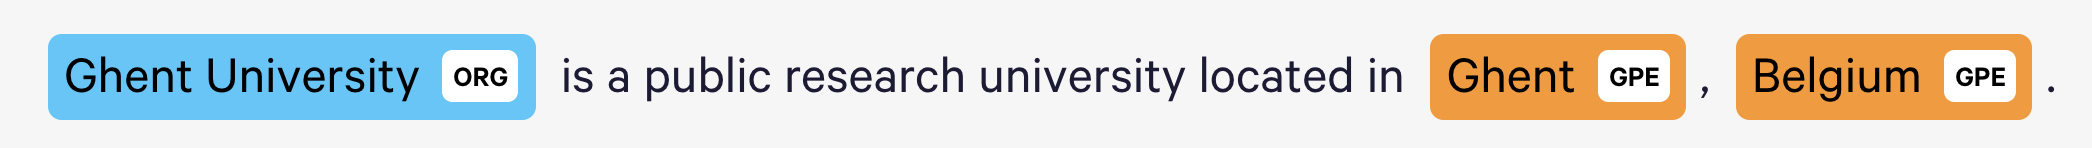
\includegraphics[width=1\linewidth]{images/ner_example} 

}

\caption{An example of a simple NER task with the \href{https://explosion.ai/demos/displacy-ent}{displaCy Named Entity Visualizer}.}\label{fig:ner-example}
\end{figure}



This might appear somewhat trivial at first sight with regular string or pattern matching and a list of known entities, but there are quite some challenges involved. These are for example related to the fact that many words have different meanings (Washington, Apple, Jobs) and that many entities span several words which makes defining their boundaries difficult - even for humans (the New England Journal of Medicine, Swiss Federal Polytechnic School, etc\ldots{}). NER is essentially a classification problem. The sequential nature of languange renders some algorithms more suited for the task than others. Today, most NER systems are based on neural networks, as discussed in chapter \ref{methods}. However, no matter which architecture is used, in order to render a NER classifier able to learn how to recognize named entities in text, the input representations must encode the semantic and syntactic properties of words in some meaningful way. Not surprisingly, a lot of the progress in the performance of NER (or any other NLP task) during the past few decades can be attributed to methods that provide these meaningful word representations.

\hypertarget{static-word-representations}{%
\section{Static word representations}\label{static-word-representations}}

Possibly the simplest solution to represent words in a quantitative way would be to use a single one-hot vector \(\mathbf{w} \in \mathbb{R}^{|V|}\) for every word in a given vocabulary of size \(|V|\), for example:

\begin{align}
\mathbf{w}_{aardvark} = [\ 1\ 0\ 0\ ...\ 0\ 0\ ...\ 0\ 0\ ]^T \notag \\
\mathbf{w}_{cat} = [\ 0\ 0\ 0\ ...\ 1\ 0\ ...\ 0\ 0\ ]^T \notag \\
\mathbf{w}_{zoo} = [\ 0\ 0\ 0\ ...\ 0\ 0\ ...\ 0\ 1\ ]^T \notag 
\end{align}

This obviously has some limitations: with arguably millions of words in the English language, these vectors are extremely sparse. Secondly, any 2 one-hot vectors are orthogonal and do not encode concepts like semantic similarity:

\[
\mathbf{w}_{cat}^T \mathbf{w}_{dog} = \mathbf{w}_{cat}^T \mathbf{w}_{airplane} = 0
\]

It is not unreasonable to assume that there must exist some \(n\)-dimensional hyperspace (with \(n\) much lower than the size of the entire English vocabulary) that can encode all semantics of a language. Many techniques have been proposed to encode words in a real-numbered space, with the two primary families being matrix factorization methods (such as latent semantic analysis (LSA) \citep{deerwester1990}) and iteration based methods based on local context (such as word2vec \citep{mikolov2013}). A key concept that many of these different methods have in common is the idea of \emph{distributional similarity}, an important hypothesis in linguistics (popularized by the British linguist J.R. Firth \citep{firth1957}) that words with a similar meaning occur in a similar context and \emph{vice versa}.

Matrix factorisation methods typically involve constructing a large matrix - often based on co-occurance counts of words in documents or smaller context windows. Then, dimension-reduction techniques such as truncated singular value decomposition are used to compress the information and obtain low-dimensional vector representations for all words in the vocabulary. Alternatively, iteration-based methods rely on neural networks that learn iteratively how to represent words in a meaningful way. A major breakthrough - in particular with respect to computational efficiency - was the development of the word2vec framework in 2013 by a team at Google \citep{mikolov2013}. The word2vec model is essentially trained to predict whether words are likely to occur together. It appeared that optimizing the model for this task yielded excellent word embeddings, with the vector representations of semantically similar words being oriented closely together in the high-dimensional embedding space. In addition, the relative orientation of the word vectors in the embedding space even showed to encode meaningful semantic or syntactic concepts, illustrated by the low-dimensional linear mappings of some word embeddings shown in Figure \ref{fig:w2v}. Other widely-used word vectors include Stanford's typically low-dimensional (50-100) GloVe vectors \citep{pennington2014} that are partly based on word co-occurence count matrices, or Facebook's 100-300-dimensional fastText vectors \citep{bojanowski2017, joulin2017}.

A problem with these static word embeddings is that words that were not encountered during training don't have an embedding. A possible solution is to learn subword embeddings. The intuition is straightforward: the suffix \emph{-shire} lets you guess that Melfordshire is probably a location, or the suffix \emph{-osis} that Myxomatosis might be a sickness\footnote{\href{https://nlp.h-its.org/bpemb/\#}{Example taken from: https://nlp.h-its.org/bpemb/}}. Subword-based embeddings have been developed by e.g.~fastText through representing words as bags of \(n\)-grams \citep{bojanowski2017}. This largely solves the problem of these out-of-vocabulary words but results in huge models. An arguably more elegant solution for this problem is provided by BytePair encoding, an unsupervised tokenization algorithm that iteratively merges frequent pairs of characters for a fixed number of iterations \citep{sennrich2016}. Applying this algorithm on a large corpus of text for a well-chosen number of iterations typically yields reasonable subword segementations, where frequent words are represented as such, and rare words as subword tokens. When these tokens are subsequently used to learn embeddings, the resulting BytePair embeddings appear to perform very well when used as input for different NLP tasks.

An alternative approach to obtain word embeddings is to train representations from scratch on a specific task like NER. One can for example use one hot encoded representations as input, and learn embeddings of any length by including randomly-initialized vectors as parameters of the NER classifier. Alternatively, one can use character-feature embeddings learned directly from the NER training data, as described in \citep{lample2016}. We will refer to these task-specific representations as one hot word type embeddings (OHEs) and character embeddings, respectively, and discuss them further in chapter \ref{methods}. However, learning these task-specific representations from scratch for every NER task is not very efficient and a much more successful approach is to use contextualized word representations obtained from pretrained neural LMs, as discussed below.

\begin{figure}

{\centering 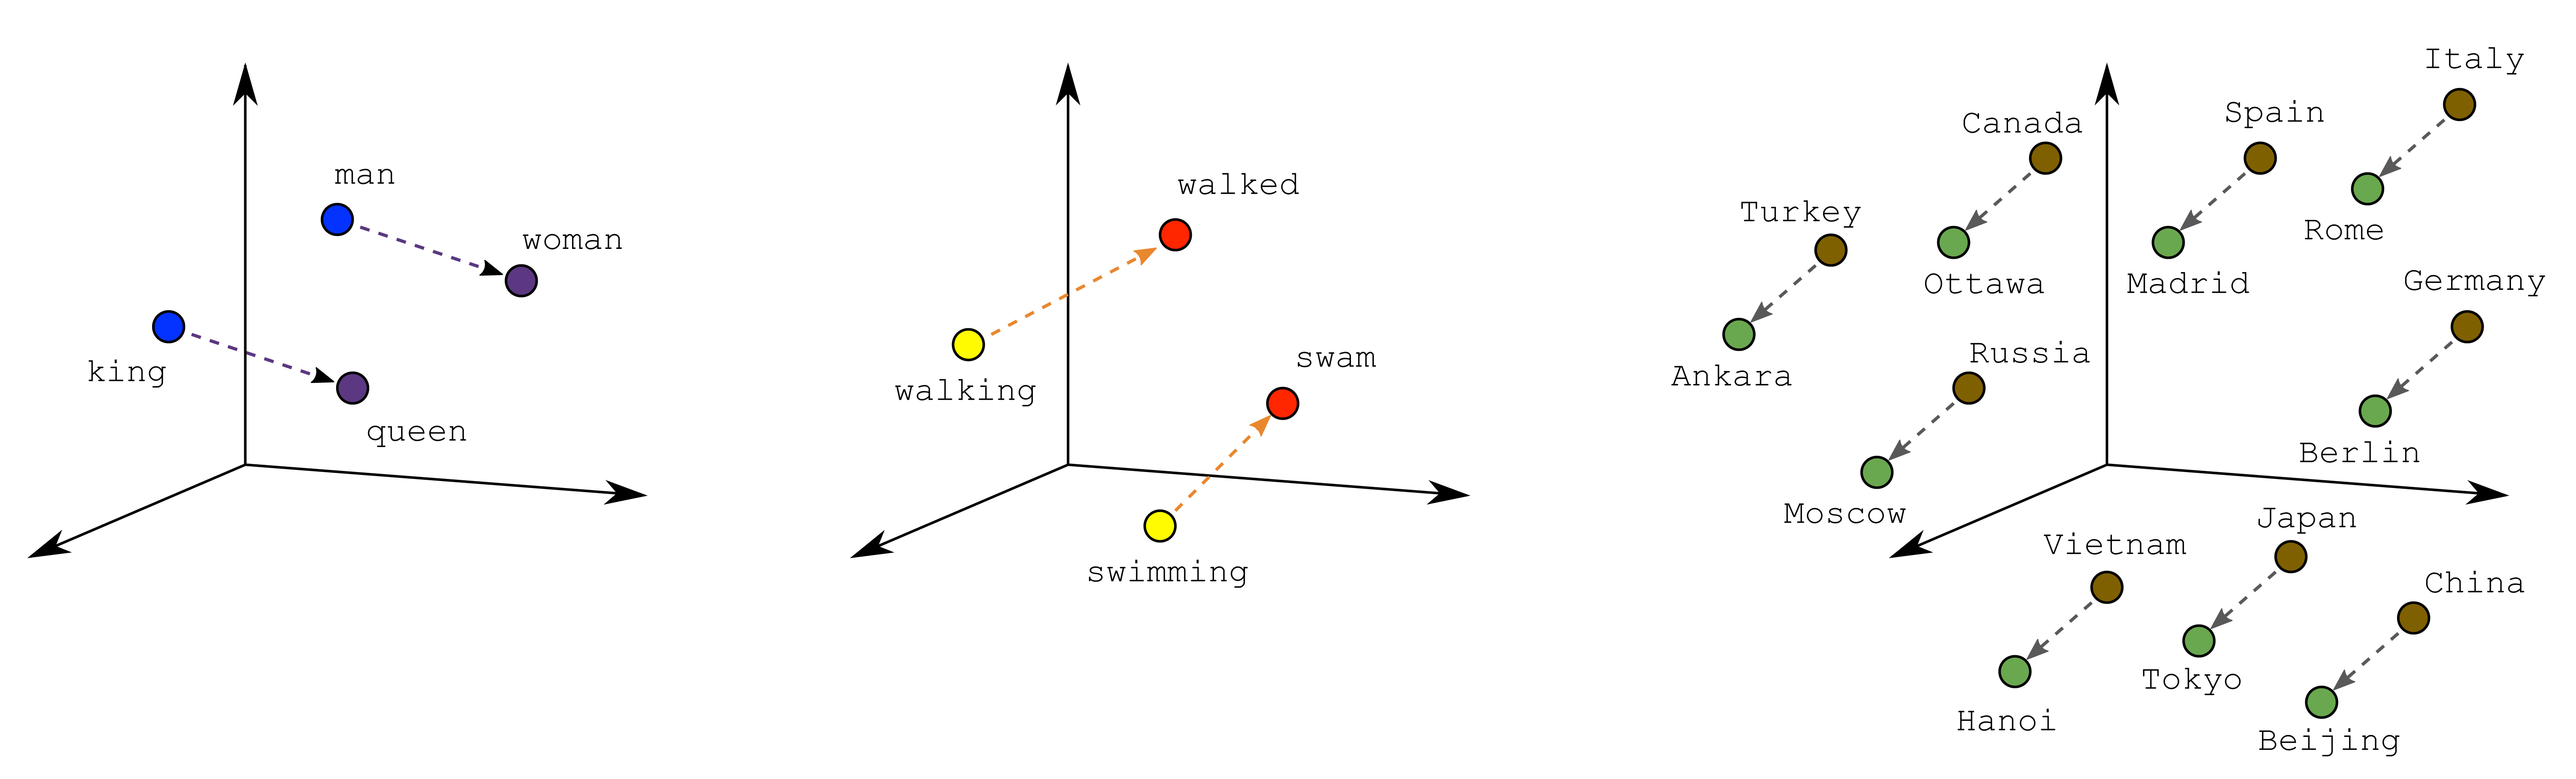
\includegraphics[width=1\linewidth]{images/word_vectors} 

}

\caption{Low-dimensional linear mappings of word vectors elegantly demonstrate how the learned dimensions effectively encode meaningful semantic or syntactic concepts like ``gender'' (left), verb tense (middle) or country-capital relationships (right). Taken from \url{shorturl.at/ivz38}.}\label{fig:w2v}
\end{figure}



\hypertarget{contextualized-word-representations-and-language-models}{%
\section{Contextualized word representations and language models}\label{contextualized-word-representations-and-language-models}}

Static word embeddings like word2vec and fastText led to significant improvements in the NLP field during the past decade. They provide a lot of meaningful information that can often not be learned from scratch from a training dataset of limited size. However, they suffer from a major limitation: many words have different meanings and these static word embeddings aggregate all these different meanings into a single vector \citep{arora2018}. This is especially problematic for polysemous words like ``play'', ``Washington'' or ``mouse''. These issues have been addressed in the recent years with the development of so-called contextualized word embeddings - i.e.~embeddings that represent words in their context, meaning that a single polysemous word like ``Washington'' has a different word embedding, depending on the context it appears in.

A key concept to learn these contextualized representations is the idea of a LM. LMs are probabilistic classifiers that are trained to predict the probability of a word given the previous words. LMs have played a crucial role in NLP for many decades (long before the rise of deep learning) as they allow to predict words given some context or can provide probabilities of word sequences (Equation \eqref{eq:chainrule}). A good LM will thus assign a higher probability to the sequence ``I like bikes'' as compared to ``Airplane cat want is'' because the former sequence is semantically and syntactically valid, while the latter sequence makes no sense. This renders them very useful for many NLP tasks. Yet, the underlying idea of the LM objective is surprisingly simple. The joint probability of a sequence of \(m\) words (\({w_1, w_2, ..., w_m}\)) can be decomposed into a product of conditional probabilities \citep{jurafsky2019}:

\begin{equation}
P\left(w_1, ..., w_m\right) = \prod_{i=1}^m P\left(w_i\mid w_1, ..., w_{i-1}\right)
\label{eq:chainrule}
\end{equation}

A so-called forward LM is trained to estimate the conditional probability of a word \(w_i\) given the previous words \({w_1,..., w_{i-1}}\). Since the number of all possible word sequences for a vocabulary of size \(|V|\) is \(|V|^m\), estimating these conditional probabilities by simply counting how often every sequence (\(w_1,..., w_{i-1}\)) is followed by \(w_i\) in a corpus is practically impossible. Traditionally, this was often solved by approximating the entire history of a word by a fixed window of size \(n - 1\) (with n typically not larger than 5):

\begin{equation}
P\left(w_1, ..., w_m\right) \approx \prod_{i=1}^mP\left(w_i \mid w_{i - n + 1}, ..., w_{i-1}\right)
\end{equation}

This so-called Markov assumption \citep{manning2019} reduces the number of all possible sequences from \(|V|^m\) to \(|V|^n\), making it practically feasible to estimate these conditional probabilities by obtaining relative counts of all \(n\)-grams in a corpus. Even though it is clear that the Markov assumption is not strictly valid for language, these so-called \(n\)-gram models work surprisingly well, are very efficient to train and, hence, still used for some applications today.

However, for many NLP tasks, having access to information that might be arbitrarily far away in the sequence is required to perform well, and \(n\)-gram models are intrinsically limited in terms of the context they can consider. Luckily, more complex model architectures like Recurrent Neural Networks (RNNs), Long Short-term Memory (LSTM) or Transformers are able to handle much longer histories, rendering them much better at the LM task. These architectures will be discussed in chapter \ref{methods}. There has been a steady rise in the quality and applications of (deep) neural LMs over the past 1-2 decades, with modern neural LMs being able to internalize an incredible amount of linguistic knowledge from huge corpora of text. While there are major differences in terms of the neural architectures and training algorithms, a key concept that drives a lot of these models' ability to internalize linguistic knowledge is the LM task: predicting a word given some context as input. When trained well, these models are able to provide probability distributions over word sequences or predict words when given some context, rendering them extremely useful in applications such as auto-completion tasks, text generation, machine-translation or speech recognition. In addition, the contextual information (that may extend back to the very beginning of the sequence) that is considered by the model to predict the next word is essentially encoded in the hidden states of these neural LMs. Recent attempts to use these representations as contextualized word embeddings for different NLP tasks - including NER - have been very successful, as discussed in chapter \ref{methods}.

\hypertarget{monolingual-versus-multilingual-embeddings}{%
\section{Monolingual versus multilingual embeddings}\label{monolingual-versus-multilingual-embeddings}}

Today, pretrained static word embeddings like word2vec \citep{mikolov2013}, fastText \citep{bojanowski2017} and GloVe \citep{pennington2014} are available for a wide range of languages. Similarly, many of the previously discussed neural LMs provide contextualized word representations. The recently developed character-based Flair LM \citep{akbik2018} or Transformer-based BERT model \citep{devlin2019} (both models are discussed in chapter \ref{methods}) have been pre-trained in several languages and are often made freely available. Examples include CamemBERT \citep{martin2019} and BERTje \citep{devries2019}, a French and Dutch version of BERT, respectively, or the Dutch and French versions of Flair made available in the \href{https://github.com/flairNLP/flair/blob/master/resources/docs/embeddings/FLAIR_EMBEDDINGS.md}{Flair's NLP library}.

These previously-discussed frameworks provide word representations in a monolingual semantic space. As mentioned previously, this has some limitations that are directly related to the research problems formulated earlier. For example, implementing an existing NLP task for a similar problem in a different language involves starting from scratch. Training and maintaining multiple pipelines for different languages has to be done independently. Many words - especially named entities - are similar across languages, suggesting that having different independent monolingual embeddings to represent these entities in different languages might not be very efficient. Additional problems with monolingual embeddings arise when the input data is multilingual.

These problems have been partly addressed through unsupervised or semi-supervised algorithms that jointly map monolingual word embeddings into a common multilingual embedding space such that words with a similar meaning are aligned \citep{artetxe2018, lample2018}. In addition, the aforementioned BytePair encoding algorithm has been used to create (static) multilingual BytePair embeddings based on a single corpus of Wikipedia articles in 275 languages \citep{heinzerling2017}. With the efficiency of BERT's transformer architecture and Flair's character-based LM objective, the question then arises whether these models can be jointly trained over a large corpus of text in many different languages to learn contextualized encodings for a multilingual vocabulary in a single embedding space without having to explicitely align different monolingual embeddings. This has been attempted for both the BERT and Flair models: multilingual BERT (mBERT)\footnote{\href{https://github.com/google-research/bert/blob/master/multilingual.md}{GitHub: google-research/bert/multilingual}} was trained on a corpora consisting of the 100 most common languages on Wikipedia and the multilingual version of Flair (mFlair) was trained on over 300 languages\footnote{\href{https://github.com/stefan-it/flair-pos-tagging}{Github: stefan-it/flair-pos-tagging}}. Since a single multilingual vocabulary was provided as training data, these models are hypothesized to learn word meaning in a language-independent way such that the vector representations for e.g. \emph{vélo}, \emph{bike} and \emph{fiets} are located close to each other in the embedding space. A potential application for such language-independent semantic representations is so-called zero-shot cross-lingual model transfer. This involves training a downstream task like NER using data from a high-resource language like English and effectively applying the learned classifier in another language like Dutch. Experiments with mBERT have shown that this approach works surprisingly well, indicating that different mBERT embeddings share a significant subspace that encodes semantic information in a language-independent way \citep{pires2019}.

\hypertarget{summary}{%
\section{Summary}\label{summary}}

In this thesis, we aim to evaluate how state-of-the-art monolingual and monolingual embeddings affect the performance of different NER tasks. To challenge the research hypotheses mentioned at the beginning of this chapter, we will use both monolingual and multilingual datasets to train and evaluate NER classifiers using different embedding types. In order to acquire a better understanding on how different embedding types affect NER performance, we will not only evaluate single monolingual and multilingual embeddings, but also create so-called stacked embeddings by concatenating different static, task-specific and contextualized word representations into a single, high-dimensional embedding vector.

\hypertarget{methods}{%
\chapter{Methods}\label{methods}}

\hypertarget{data}{%
\section{Data}\label{data}}

\hypertarget{benchmark-datasets}{%
\subsection{Benchmark datasets}\label{benchmark-datasets}}

To evaluate how different monolingual and multilingual embeddings affect NER performance, we made use of large, well-annotated datasets for NER tasks. For Dutch and English, we used the shared task of respectively the 2002 and 2003 Conference on Computational Natural Language Learning (CoNLL) \citep{tjongkimsang2002, tjongkimsang2003}. These widely used benchmarks datasets for Dutch and English NER consist of separate train, development and test sets of human-annotated, tokenized sentences from news articles from \href{https://trec.nist.gov/data/reuters/reuters.html}{Reuters Corpus} (English CoNLL 2003) and four editions of the Belgian newspaper ``De Morgen'' of the year 2000 (Dutch CoNLL2002). For French, the WikiNER dataset (wiki-3 version) was used \citep{nothman2013}. This dataset relied on automatic NER annotation algorithms based on Wikipedia's article metadata as well as some additional heuristics, which has been shown to yield excellent-quality NER annotations. Because this dataset is much larger as compared to the CoNLL datasets, we used a random sample of 10 \% of the entire dataset to approximately match the size of the CoNLL datasets (Table \ref{tab:benchmark-ds}).

We maintained the train, development and test split of the original CoNLL datasets. The CoNLL2002 dataset contained a low number of relatively long sentences. Since some of the Transformer architectures used to obtain contextualized token representations (cf infra) have a limited input sequence length, the sentences exceeding 250 tokens were excluded. This resulted in the removal of 4/15806 sentences from the training set and 1/5195 sentences in the test set.

All three datasets were pre-labelled with 4 different NER tags: persons (PER), organizations (ORG), locations (LOC) and miscellaneous names (MISC), they were all converted to the same BIO2 format according to the original CoNLL2002 dataset \citep{tjongkimsang2002}. This means that every line represented a word token and the NER tag, prefixed with either ``B-'' (``beginning'') or ``I-'' (``inside'') for respectively the first and subsequent tokens of entities spanning multiple tokens. Single-token entities were prefixed with ``B-'', all other tokens were tagged with the label ``O'' (``other''). Different sentences were separated by a blank line. Indicators of document boundaries, such as the DOCSTART token in the CoNLL datasets, were removed. An example sentence from the Dutch CoNLL2002 dataset is given below.

\begin{Shaded}
\begin{Highlighting}[]
\ExtensionTok{Onder}\NormalTok{ O}
\ExtensionTok{de}\NormalTok{ O}
\ExtensionTok{bruuske}\NormalTok{ O}
\ExtensionTok{tempoversnellingen}\NormalTok{ O}
\ExtensionTok{van}\NormalTok{ O}
\ExtensionTok{Gilberto}\NormalTok{ B-PER}
\ExtensionTok{Simoni}\NormalTok{ I-PER}
\ExtensionTok{op}\NormalTok{ O}
\ExtensionTok{de}\NormalTok{ O}
\ExtensionTok{steilste}\NormalTok{ O}
\ExtensionTok{gedeelten}\NormalTok{ O}
\ExtensionTok{van}\NormalTok{ O}
\ExtensionTok{de}\NormalTok{ O}
\ExtensionTok{Pratonevoso}\NormalTok{ B-LOC}
\ExtensionTok{moest}\NormalTok{ O}
\ExtensionTok{Casagrande}\NormalTok{ B-PER}
\ExtensionTok{passen}\NormalTok{ O}
\BuiltInTok{.} \ExtensionTok{O}
\end{Highlighting}
\end{Shaded}

In addition to these three monolingual dataset, we combined them into a single trilingual dataset to perform multilingual NER. For efficiency reasons, the combined dataset was obtained by randomly sampling one third of the sentences from each monolingual dataset (maintaining the same train, development and test splits). The specific datasets used here - together with all the code to reproduce the experiments - are made available on the GitHub repository of this thesis (\href{https://github.com/arthur-arthur/NER}{arthur-arthur/NER}). The English CoNLL2003 dataset requires a licence from \href{https://trec.nist.gov/data/reuters/reuters.html}{Reuters Corpus} (free for research purposes) and was therefore not included in the repository.

\begin{table}

\caption{\label{tab:benchmark-ds}Overview of the characteristics of the train, development (dev) and test benchmark datasets used to evaluate different monolingual and multilingual embeddings on monolingual and multilingual NER tasks. The WikiNER dataset was downsampled to roughly match the size of the Dutch and English datasets, the multilingual datasets was created by randomly sampling 1/3th of every monolingual dataset (maintaining the same train, dev and test splits).}
\centering
\begin{tabular}[t]{llrrrrrr}
\toprule
\multicolumn{2}{c}{ } & \multicolumn{3}{c}{\# sentences} & \multicolumn{3}{c}{\# tokens} \\
\cmidrule(l{3pt}r{3pt}){3-5} \cmidrule(l{3pt}r{3pt}){6-8}
 &  & Train & Dev & Test & Train & Dev & Test\\
\midrule
En & CoNLL03 & 14041 & 3250 & 3453 & 203621 & 51362 & 46435\\
Nl & CoNLL02 & 15802 & 2895 & 5194 & 199969 & 37687 & 68466\\
Fr & WikiNER & 10713 & 1190 & 1323 & 279729 & 34824 & 30991\\
Multi & Multilingual & 13518 & 2444 & 3323 & 232173 & 40141 & 49444\\
\bottomrule
\end{tabular}
\end{table}

\hypertarget{faktion-datasets}{%
\subsection{Faktion datasets}\label{faktion-datasets}}

In addition to these well-validated benchmark datasets, similar experiments were performed on smaller ``real-word'' datasets that were obtained from Metamaze, the document annotation application developed by Faktion. The data consisted of text obtained with an in-house developed optical character recognition (OCR) pipeline on relatively poor quality scans of building plans. Hence, many of the tokens consisted of a single character or only punctuation, resulting in long sequences and many tokens with little semantic information. The data were user-annotated within the Metamaze application, i.e.~based on the location of the tokens in the document scans, not on the text output from the OCR pipeline itself. Given the limited input sequence length of some of the Transformer models, we reduced the average sequence length (i.e.~tokens per document) by removing all tokens that consisted of punctuation only. Another difference with the benchmark datasets described earlier was the number of NER labels to predict: while there were 4 different entity labels in the CoNLL and WikiNER datasets (PER, LOC, ORG and MISC), there was only a single category (``naam\_bouwplan'') in the Dutch Faktion dataset, and only one additional category (``naam\_bouwplan\_2'') in the French dataset, with approximately 95\% of all entities belonging to a single category. A representative fragment of the OCR output for one of the documents (after preprocessing) is given below:

\begin{Shaded}
\begin{Highlighting}[]
\ExtensionTok{310}\NormalTok{ B-naam_bouwplan}
\ExtensionTok{4}\NormalTok{ I-naam_bouwplan}
\ExtensionTok{Lewsrass}\NormalTok{ O}
\ExtensionTok{wes}\NormalTok{ O}
\ExtensionTok{BATIMENT}\NormalTok{ B-naam_bouwplan}
\ExtensionTok{A}\NormalTok{ I-5e57}
\ExtensionTok{aren}\NormalTok{ O}
\ExtensionTok{seres}\NormalTok{ O}
\ExtensionTok{Meg}\NormalTok{ O}
\ExtensionTok{names}\NormalTok{ O}
\ExtensionTok{808}\NormalTok{ O}
\ExtensionTok{0e}\NormalTok{ O}
\ExtensionTok{side}\NormalTok{ O}
\ExtensionTok{panama}\NormalTok{ O}
\ExtensionTok{VERDIERING}\NormalTok{ B-naam_bouwplan}
\ExtensionTok{3}\NormalTok{ I-naam_bouwplan}
\ExtensionTok{-}\NormalTok{ I-naam_bouwplan}
\ExtensionTok{3}\NormalTok{ I-naam_bouwplan}
\ExtensionTok{1ewe}\NormalTok{ I-naam_bouwplan}
\ExtensionTok{E74}\NormalTok{ I-naam_bouwplan}
\ExtensionTok{A}\NormalTok{ O}
\ExtensionTok{0e}\NormalTok{ O}
\ExtensionTok{58}\NormalTok{ O}
\ExtensionTok{A0}\NormalTok{ O}
\ExtensionTok{03}\NormalTok{ O}
\end{Highlighting}
\end{Shaded}

Another important characteristic of these datasets was that none of them were strictly monolingual. The language was decided on the dominant language (Table \ref{tab:faktion-ds}). A third - bilingual - dataset was created by merging the French and Dutch datasets. Given the characteristics of the datasets and, hence, the expected imprecision of the extra-sample error estimates, all experiments were repeated 5 times on independent random (80/20) splits of the data.

\begin{table}

\caption{\label{tab:faktion-ds}Number of sequences (documents) and tokens per train, development (dev) and test splits for the Dutch (Nl), French (Fr) and multilingual Faktion datasets. The reported values are the averages of the 5 independent random splits. Note that even the monolingual datasets contained bilingual documents, the language was chosen based on the dominant language in each dataset.}
\centering
\begin{tabular}[t]{llrrrrrr}
\toprule
\multicolumn{2}{c}{ } & \multicolumn{3}{c}{\# documents} & \multicolumn{3}{c}{\# tokens} \\
\cmidrule(l{3pt}r{3pt}){3-5} \cmidrule(l{3pt}r{3pt}){6-8}
 & \% bilingual & Train & Dev & Test & Train & Dev & Test\\
\midrule
Nl & 58 & 21 & 9 & 6 & 2619 & 1062 & 789\\
Fr & 9 & 91 & 32 & 29 & 9706 & 3273 & 3131\\
Multi &  & 112 & 40 & 36 & 11976 & 4435 & 4171\\
\bottomrule
\end{tabular}
\end{table}

\hypertarget{word-embeddings}{%
\section{Word embeddings}\label{word-embeddings}}

\hypertarget{static-and-task-specific-embeddings}{%
\subsection{Static and task-specific embeddings}\label{static-and-task-specific-embeddings}}

As introduced in the previous chapter, there are a wide range of possible methods to obtain word representations that allow to perform NER. Static word embeddings like word2vec or fastText have had a significant impact on the performance of NER systems and have long been the default choice for many NLP tasks, including NER. They are still used today in combination with contextualized representations to provide state-of-the-art performance \citep{akbik2018}. We included two types of static word embeddings, i.e.~monolingual fastText word embeddings (English, Dutch and French) as well as monolingual BytePair and multilingual BytePair (mBytePair) embeddings (Table \ref{tab:embeddings}), as discussed previously.

In addition, two types of task-specific representations were obtained. This included one hot word type embeddings (OHEs) that were obtained by encoding all words in the vocabulary as one hot vectors and introducing an embedding layer into the network to obtain 300-dimensional word type representations\footnote{\url{https://github.com/flairNLP/flair/blob/master/resources/docs/embeddings/ONE_HOT_EMBEDDINGS.md}}. In addition, we obtained 50-dimensional task-specific representations based on character-features\footnote{\url{https://github.com/flairNLP/flair/blob/master/resources/docs/embeddings/CHARACTER_EMBEDDINGS.md}}, as described in \citep{lample2016}. The OHEs were included to confirm the well-established idea on the differences between learning word embeddings from scratch on the NER objective and using representations from pretrained LMs. The character-feature embeddings were included because they have been shown to improve NER performance when concatenated to other word representations \citep{akbik2018, lample2016}. Both these task-specific representations were evaluated in the context of both monolingual and multilingual embeddings (Table \ref{tab:embeddings}).

\hypertarget{contextualized-word-embeddings}{%
\subsection{Contextualized word embeddings}\label{contextualized-word-embeddings}}

Even though static and/or task-specific representations have long been the default, today, all state-of-the-art NER systems rely on some form of contextualized word representation obtained from a pretrained neural LM. Below, we briefly discuss some neural network architectures and LMs that played an important role in the progress of the field during the recent years, how these models can be used to obtain multilingual word embeddings and which embedding types were used for the experiments presented in this thesis.

\hypertarget{recurrent-neural-networks}{%
\subsubsection{Recurrent Neural Networks}\label{recurrent-neural-networks}}

Recurrent Neural Networks (RNN) are a class of neural network architectures that deal especially well with the sequential nature of natural language. In contrast to traditional neural networks, the hidden layer units do not simply pass their states along to input-output axis (i.e.~from the input layer to the output layer), but pass the output of every unit to the next unit within that same layer. An example for a simple RNN LM is given in Figure \ref{fig:rnnlm} (example taken from \citep{manning2019}). For this example, the RNN has to predict the next word in the sentence (``The students opened their''), i.e.:

\begin{equation}
P\left(w_5\mid the, \ students, \ opened, \ their\right) \notag
\end{equation}

First, words are represented as one-hot vectors \(\mathbf{w}_i \in \mathbb{R}^{|V|}\) with \(i\) indicating the position of the word in the sequence. Then, an embedding matrix \(\mathbf{E} \in \mathbb{R}^{d \times |V|}\) is used to obtain static \(d\)-dimensional word embeddings like word2vec \citep{mikolov2013}.

\begin{equation}
\mathbf{e}_i = \mathbf{E}\mathbf{w}_i \notag
\end{equation}

The hidden state for every unit \(\mathbf{h}_i\) is computed as a linear combination of the word vector for the \(i\)-th word in the sequence, \(\mathbf{e}_i\), as well as the hidden state from the previous unit \(\mathbf{h}_{i-1}\). This is passed through a nonlinear activation function \(\sigma\), just like a regular feed-forward neural network:

\begin{equation}
\mathbf{h}_i =  \sigma (\mathbf{W}_h \mathbf{h}_{i-1} + \mathbf{W}_e \mathbf{e}_{i}) \notag
\end{equation}

Lastly, a linear combination of the last hidden state \(\mathbf{h}_{4}\) (that encodes information on the last input word, as well as the entire past context) is passed through a softmax activation function \citep{goodfellow2016} (i.e.~essentially performing multinomial logistic regression) to predict a probability distribution over the vocabulary (\(\mathbf{\hat{y}}_4 \in \mathbb{R}^{|V|}\)) for the last word \(\mathbf{w}_5\), i.e.~more generally:

\begin{equation}
\mathbf{\hat{y}}_i =  softmax (\mathbf{W}_o \mathbf{h}_{i}) \notag
\end{equation}

with \(\mathbf{W}_e\), \(\mathbf{W}_h\), \(\mathbf{W}_o\) being the weight matrices to be learned by the network (biases are omitted). Introducing the matrix \(\mathbf{W}_h\) allows the network to learn how to make use of this past context (encoded in \(\mathbf{h}_{i-1}\)) while computing the output of its current state. Since the weight matrix \(\mathbf{W}_h\) is shared across all timesteps, the length of the input sequence does not increases the model size in terms of parameters. While the aforementioned \(n\)-gram language models are constrained by the incorrect assumption that a given word only depends on a limited number of previous words, RNNs can effectively consider \emph{all} preceding words, making them well-suited for the LM task.



\begin{figure}

{\centering 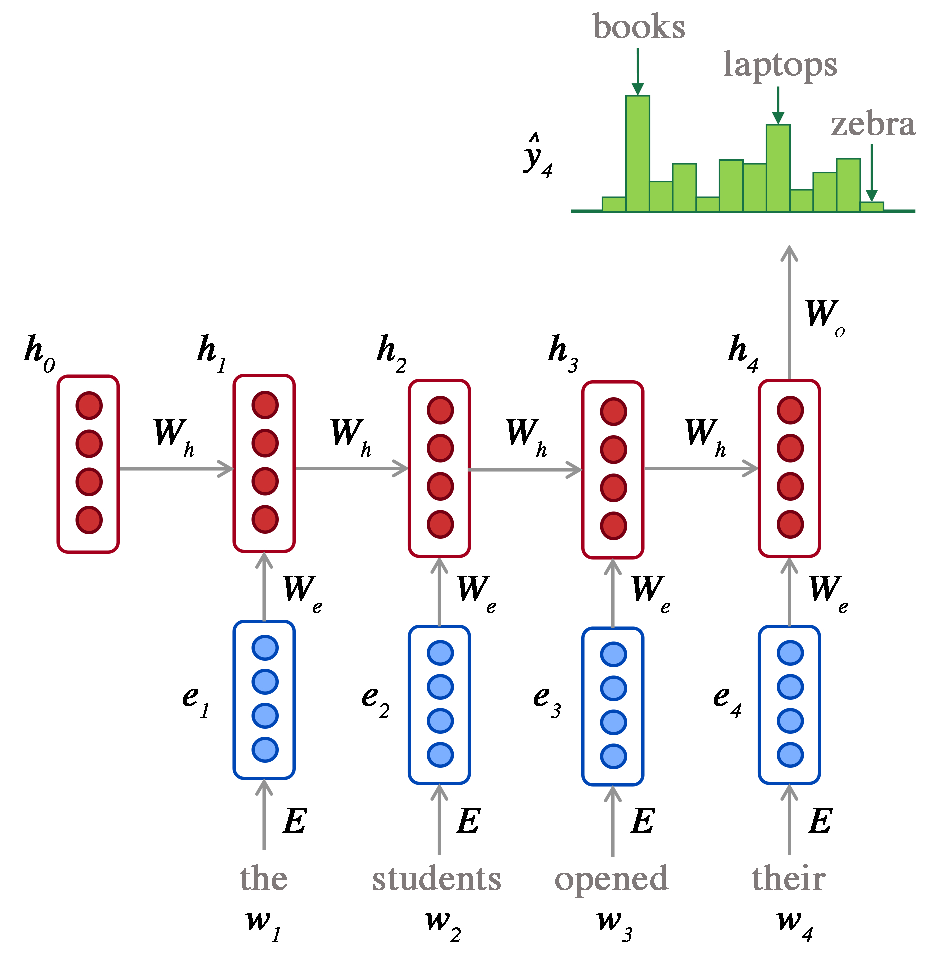
\includegraphics[width=0.75\linewidth]{images/RNN_LM} 

}

\caption{A schematic representation of a simple RNN LM with a single hidden layer. The output is passed through a softmax layer to generate a probability distribution over the entire vocabulary. The model is trained in a completely unsupervised way through minimizing the cross-entropy loss, i.e.~the negative log probability that the model assigned to the correct word. This conceptually very simple idea forms the foundation of many state-of-the-art neural LMs that are used today. Adapted from \citep{manning2019a}.}\label{fig:rnnlm}
\end{figure}

Unfortunately, in practice, RNN tend to encode relatively local information in their hidden states. The backpropagation step during training involves computing gradients and multiplying these (since the loss at a given time step is a function of the previous hidden state in the sequence). When the number of units in the sequence increases, these sequential multiplications can easily result in very large or very small numbers, a phenomenon commonly referred to as exploding or vanishing gradients, respectively \citep{bengio1993}. Since the model parameters are iteratively updated according to this gradient, this can cause the algorithm to diverge or dramatically slow down the learning process.

\hypertarget{long-short-term-memory-models}{%
\subsubsection{Long Short Term Memory models}\label{long-short-term-memory-models}}

Long Short Term Memory (LSTM) networks involve an additional level of architectural complexity and expand the parameter space, but provide an elegant solution to the aforementioned vanishing gradient issue. They learn how to actively manage contextual information in a so-called ``memory-cell'' - an additional vector that encodes historical information. The model is allowed to learn how to efficiently manage this historical information by parametrizing it with its own set of weights that control the flow of information in and out of the units of the hidden layers. This renders LSTMs better at handling contextual information and encoding long-range dependencies in its hidden states, as compared to simple RNNs \citep{goodfellow2016}. LSTMs are widely used for many applications, including classification tasks such as NER. In fact, one of the best-performing NER classifier models today is based on a LSTM and this specific architecture was used for the experiments presented in this thesis. A schematic overview of this architecture is given in Figure \ref{fig:bilstmcrf}. In addition, the ability of LSTMs to effectively model very long-range dependencies generally translates into excellent performance on the LM task. Today, many deep neural LMs consist of stacked layers of sequential LSTM units, and are often (independently) optimized for two objectives: to predict a word given the previous words, and to predict a word given the next words. Combining these forward and backward LMs yield so-called BiLSTM LMs that are used in many NLP applications, such as text autocompletion tasks, machine translation or speech recognition. In addition, their hidden states provide excellent contextualized word embeddings, as dicussed below.

\hypertarget{taglm}{%
\subsubsection{TagLM}\label{taglm}}

One of the first architectures to effectively exploit the hidden states of a BiLSTM LM as contextual word vectors to train a NER classifier was the TagLM model \citep{peters2017}. In short, the TagLM model made use of a large BiLSTM that was pre-trained using a large corpus of text on a LM objective. A second neural classifier was trained to perform NER. Instead of just feeding static word embeddings (e.g.~word2vec or fastText) into this classifier, or training task-specific representations from scratch on the NER objective, they fed their input sequences into the pre-trained LM and extracted the hidden states. By feeding both static word embeddings as well as the concatenated forward and backward hidden states of the LM into the NER classifier, they achieved state-of-the-art performance on the NER task (Figure \ref{fig:taglm}).

\begin{figure}

{\centering 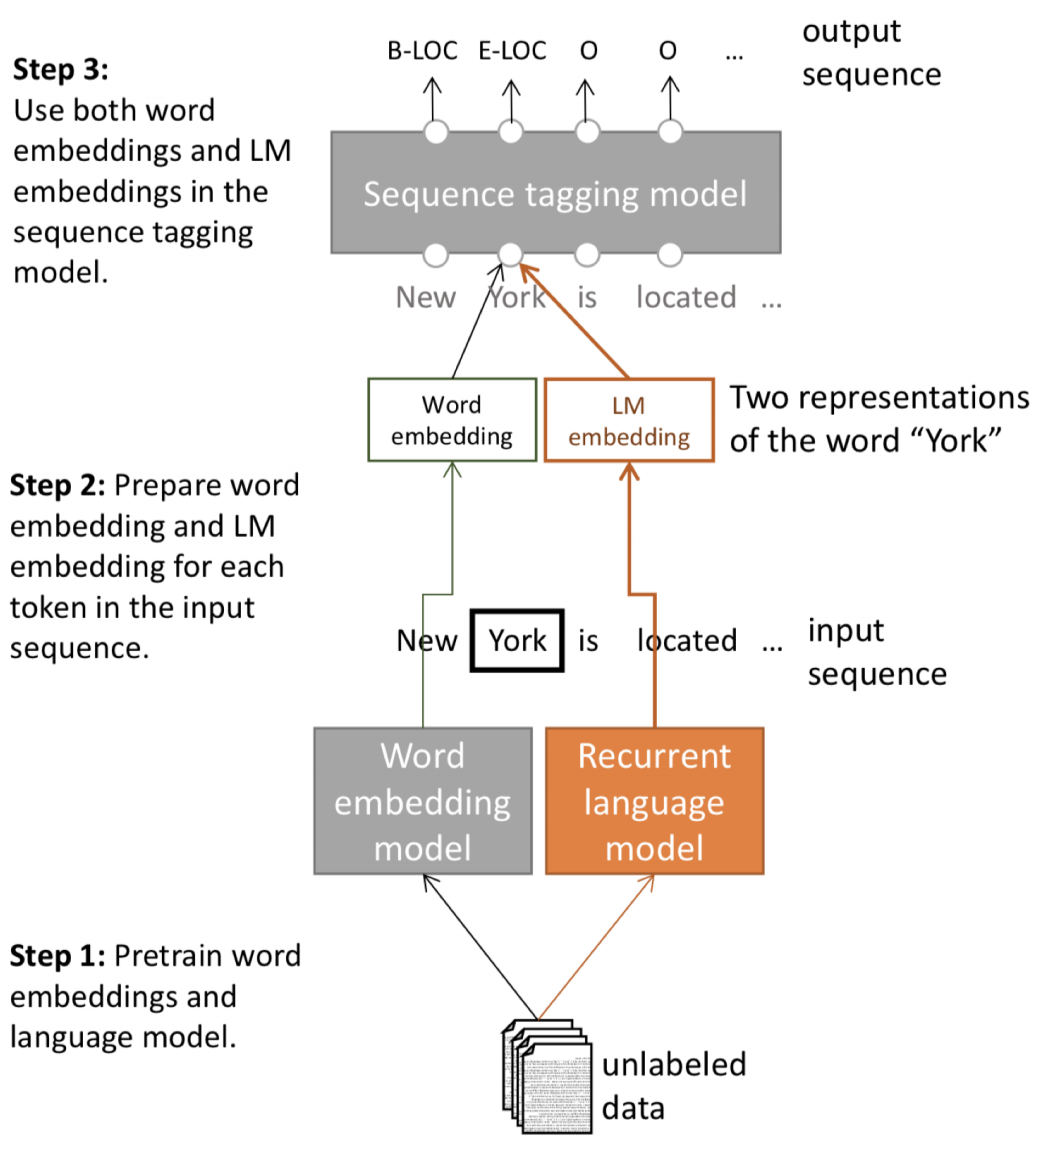
\includegraphics[width=0.85\linewidth]{images/TagLM} 

}

\caption{Schematic overview of the TagLM model. The NER task is based on both static word embeddings as well as contextualized word representations from the hidden states of a pre-trained bidirectional recurrent language model. Taken from \citep{peters2017}}\label{fig:taglm}
\end{figure}



\hypertarget{elmo}{%
\subsubsection{ELMo}\label{elmo}}

The ELMo (Embeddings from Language Models) architecture was an improved version of the TagLM model that achieved incredible performance on many NLP-tasks, including NER. ELMo is based on a deep, multi-layer BiLSTM LM to obtain context- and task-specific word representations from the hidden states of the LM layers \citep{peters2018}. The excellent performance was partly achieved through representing words as a weighted average of the internal representations of the LM. It turned out that by introducing these weights as trainable parameters of the downstream task, the downstream model can make optimal use of the semantic and syntactic information that are encoded in the different layers of the LM. ELMo embeddings were able to improve the state-of-the-art of virtually all possible NLP tasks with a very significant margin.

\hypertarget{flair}{%
\subsubsection{Flair}\label{flair}}

Another succesful approach to obtain contextual word embeddings was the Flair architecture, developed by Alan Akbik and colleagues in 2018 \citep{akbik2018}. The general idea of Flair is - again - to obtain contextual word representations from a large, pre-trained language model that can subsequently be used to train a supervised NLP task such as NER.

In contrast to ELMo, the authors used a character-based BiLSTM LM, i.e.~the model was trained to predict a character given the previous characters in the sequence (and \emph{vice versa}, since it was a bidirectional LM) - without given any explicit notion of words. When a lot of training data is provided, these models have been shown to succesfully internalize linguistic concepts such as words, sentences, grammar, punctuation and even more complex, long-range linguistic dependencies \citep{graves2014, sutskever2014}. Advantages of using a character-level language model are the improved handling of misspelled and rare words. In addition, since the ``vocabulary'' of these models is fixed and very compact (characters instead of words), these models are very efficient to train, independent from tokenization. By concatenating the internal states of the language model from both the forward and backward LSTM, they obtained context-specific word vectors, as illustrated in Figure \ref{fig:flairLM}.

\begin{figure}

{\centering 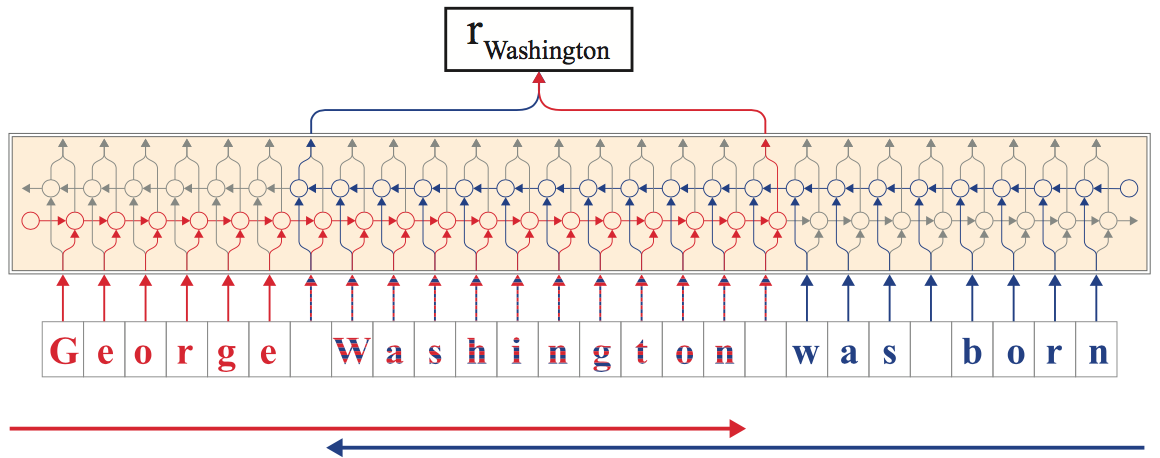
\includegraphics[width=1\linewidth]{images/flair_LM} 

}

\caption{The character-based bi-directional Flair LM yields word representations (\(\mathbf{r}\)) that contain information from the word itself, as well as from surrounding characters in the sentence, thus encoding information from the entire sequence. Taken from \citep{akbik2018}.}\label{fig:flairLM}
\end{figure}



They proposed an architecture for NER that was based on their character-based LM and a downstream BiLSTM-CRF classifier. The authors experimented with concatenating their contextual character-based word representations with `static' GloVe word embeddings as well as the task-specific character-feature embeddings discussed previously. They demonstrated that a stacked embedding containing the proposed character-level contextualized word embeddings as well as the trainable character-feature embeddings and static GloVe embeddings resulted in state-of-the-art performance on the CoNLL 2003 NER task \citep{akbik2018}.

In addition to training the aforementioned language model, the authors also released an open source PyTorch-based NLP library \citep{akbik2019b} that supports a wide range of pre-trained embeddings and LMs. The high training efficiency of the character-based LMs is one of the main reasons that several Flair LMs have been pretrained in different languages. For the experiments reported in this thesis, we used the original (English) Flair model described here, as well as the Dutch, French and multilingual versions in different configurations with other static or task/specific embeddings, as explained below (Table \ref{tab:embeddings}). The Dutch, French and multilingual versions of Flair were trained by members of the community and made freely available in the Flair library\footnote{More information on these models can be found in the \href{https://github.com/flairNLP/flair/blob/083eb114505ede0ea3070317a5a08d13fc71891b/resources/docs/embeddings/FLAIR_EMBEDDINGS.md}{documentation of flairNLP on GitHub}}.

\hypertarget{bert}{%
\subsubsection{BERT}\label{bert}}

One of the main factors driving improvement in the performance of deep neural LMs is their scale or the amount of training data they are able to learn from. Neural language modelling is an unsupervised task which means that they are not restricted by the scarcity of human-annotated data. Wikipedia or news articles provide an enormous amount of qualitative training data, which means that much of the progress in the last few years can be attributed to the efficiency and scalability of the training algorithms. Even though RNNs like LSTMs provide excellent LMs, they have a major disadvantage: the input of each hidden state relies on the output of the preceding hidden state, making them very slow to train and difficult to parallelize. A major breakthrough with respect to training efficiency of neural LMs was the development of the so-called Transformer architecture in 2017 \citep{vaswani2017}. For an overview of the Transformer architecture we refer to \href{http://jalammar.github.io/}{Jay Alammar's} excellent post \href{http://jalammar.github.io/illustrated-transformer/}{``The Illustrated Transformer''}\footnote{\href{http://jalammar.github.io/illustrated-transformer/}{jalammar.github.io/illustrated-transformer/}}. In short, the Transformer architecture completely omits the recurrent nature of RNNs, while keeping the ability to ``memorize'' contextual information. This was achieved through the introduction of an encoder-decoder architecture (typically used in machine translation tasks) and a so-called Multi-Head Attention block, a self-attention mechanism that keeps track of the relationship between input and output, allowing the netwerk to consider specific parts of the input sequence (that can be far away) to improve its performance on the LM objective. A crucial advantage of omiting the recurrency is the fact that training can be parallelized. This facilitates scaling and this is essentially what drove the steady increase in the scale of neural LMs during the past few years.

A very succesful application of the Transformer architecture was Google's BERT (Bidirectional Encoder Representations from Transformers) \citep{devlin2019}. BERT was innovative in the sense that it used a bidirectional masked LM objective. Instead of predicting a word given the previous words (or \emph{vice versa} for a backward LM objective), they randomly masked 15 \% of the words in the corpus. By training the model to predict these masked words from the entire context, the model could jointly learn from both the left and right side of the target word. This is in contrast to a BiLSTM, in the sense that both the forward and backward LM learn independently from either history or future, as illustrated in Fig. \ref{fig:bilstmcrf}. The contextualized representations learned by BERT have been used extensively in NLP - often through adding a task-specific layer on top and fine-tuning the entire BERT model on a specific NLP task. BERT or some of its many successors (ALBERTA, RoBERTa, XLM, etc\ldots{}) are able to exceed human-like performance on high-level NLP tasks like question answering\footnote{\href{https://rajpurkar.github.io/SQuAD-explorer/}{SQuAD benchmark leaderbord}}. This illustrates that these models are able to internalize a large amount of linguistic knowledge - in a completely unsupervised way - and achieve a level of natural language understanding that - for some tasks - comes very close or even exceeds the level of natural language understanding that humans are able to acquire throughout their lives.

For the experiments presented in this report, we used, for English, the \href{https://huggingface.co/bert-base-cased}{case-sensitive BERT base model} (\href{https://github.com/huggingface/transformers}{Huggingface Transformer library}\footnote{\href{https://github.com/huggingface/transformers}{GitHub: huggingface/transformers}} reference: \texttt{bert-base-cased}), the \href{https://huggingface.co/camembert-base}{CamemBERT} (\texttt{camembert-base}) model for French \citep{martin2019} and \href{https://huggingface.co/wietsedv/bert-base-dutch-cased}{BERTje} (\texttt{wietsedv/bert-base-dutch-cased}) for Dutch \citep{devries2019}. \href{https://huggingface.co/bert-base-multilingual-cased}{Multilingual BERT (mBERT)} (\texttt{bert-base-multilingual-cased}) was used to obtain multilingual embeddings. We did not perform any fine-tuning of the weights of the BERT models, but obtained contextualized token representations by extracting the activations from the top layer of the Transformer models. Since the BERT models are based on subword tokenization and the NER model operates on the token-level, we used the representations of the first subtoken as token-level embeddings, similar to the feature-based approach described in the original BERT paper \citep{devlin2019}. The dimensions of the obtained embeddings from the different BERT-models are given in Table \ref{tab:emb-dim}.

\begin{table}

\caption{\label{tab:emb-dim}Overview of the dimensions of all English (En), French (Fr), Dutch (Nl) and multilingual (Multi) word vectors used in this thesis.}
\centering
\begin{tabular}[t]{lllll}
\toprule
Embedding & En & Fr & Nl & Multi\\
\midrule
\addlinespace[0.3em]
\multicolumn{5}{l}{\textbf{Static}}\\
\hspace{1em}fastText & 300 & 300 & 300 & \\
\hspace{1em}BytePair & 100 & 100 & 100 & 3672\\
\addlinespace[0.3em]
\multicolumn{5}{l}{\textbf{Contextualized}}\\
\hspace{1em}Flair & 4096 & 2048 & 4096 & 6144\\
\hspace{1em}BERT & 768 & 768 \textsuperscript{a} & 768  \textsuperscript{b} & 4440\\
\addlinespace[0.3em]
\multicolumn{5}{l}{\textbf{Task-specific}}\\
\hspace{1em}One hot word type & 300 & 300 & 300 & 300\\
\hspace{1em}Character & 50 & 50 & 50 & 50\\
\bottomrule
\multicolumn{5}{l}{\textsuperscript{a} CamemBERT;  \textsuperscript{b} BERTje}\\
\end{tabular}
\end{table}

\newpage

\begin{landscape}\begin{table}

\caption{\label{tab:embeddings}Overview of the different embeddings evaluated in the context of English, Dutch, French and multilingual NER. The columns indicate the type of LM used to obtain contextualized embeddings (if any). The different configurations w.r.t. static and/or task-specific embedding types are indicated by the different rows. \textit{Char: character-feature embeddings; OHE: one hot word type embeddings; BPEmb: BytePair embeddings; fastT: fastText embeddings; multilingual embeddings are prefixed with 'm'}}
\centering
\fontsize{9}{11}\selectfont
\begin{tabular}[t]{llll}
\toprule
No contextualized embeddings & BERT & Flair & BERT + Flair\\
\midrule
\addlinespace[0.3em]
\multicolumn{4}{l}{\textbf{English}}\\
\hspace{1em}\color{white}{n.a.} & BERT & Flair & BERT + Flair\\
\hspace{1em}Char & BERT + Char & Flair + Char & BERT + Flair + Char\\
\hspace{1em}OHE & BERT + OHE & Flair + OHE & BERT + Flair + OHE\\
\hspace{1em}BPEmb (En) & BERT + BPEmb (En) & Flair + BPEmb (En) & BERT + Flair + BPEmb (En)\\
\hspace{1em}fastT (En) & BERT + fastT (En) & Flair + fastT (En) & BERT + Flair + fastT (En)\\
\hspace{1em}All \textsuperscript{a} & BERT + All \textsuperscript{a} & Flair + All \textsuperscript{a} & BERT + Flair + All \textsuperscript{a}\\
\addlinespace[0.3em]
\multicolumn{4}{l}{\textbf{Dutch}}\\
\hspace{1em}\color{white}{n.a.} & BERTje & Flair (Nl) & BERTje + Flair (Nl)\\
\hspace{1em}Char & BERTje + Char & Flair (Nl) + Char & BERTje + Flair (Nl) + Char\\
\hspace{1em}OHE & BERTje + OHE & Flair (Nl) + OHE & BERTje + Flair (Nl) + OHE\\
\hspace{1em}BPEmb (Nl) & BERTje + BPEmb (Nl) & Flair (Nl) + BPEmb (Nl) & BERTje + Flair (Nl) + BPEmb (Nl)\\
\hspace{1em}fastT (Nl) & BERTje + fastT (Nl) & Flair (Nl) + fastT (Nl) & BERTje + Flair (Nl) + fastT (Nl)\\
\hspace{1em}All \textsuperscript{b} & BERTje + All \textsuperscript{b} & Flair (Nl) + All \textsuperscript{b} & BERTje + Flair (Nl) + All \textsuperscript{b}\\
\addlinespace[0.3em]
\multicolumn{4}{l}{\textbf{French}}\\
\hspace{1em}\color{white}{n.a.} & CamemBERT & Flair (Fr) & CamemBERT + Flair (Fr)\\
\hspace{1em}Char & CamemBERT + Char & Flair (Fr) + Char & CamemBERT + Flair (Fr) + Char\\
\hspace{1em}OHE & CamemBERT + OHE & Flair (Fr) + OHE & CamemBERT + Flair (Fr) + OHE\\
\hspace{1em}BPEmb (Fr) & CamemBERT + BPEmb (Fr) & Flair (Fr) + BPEmb (Fr) & CamemBERT + Flair (Fr) + BPEmb (Fr)\\
\hspace{1em}fastT (Fr) & CamemBERT + fastT (Fr) & Flair (Fr) + fastT (Fr) & CamemBERT + Flair (Fr) + fastT (Fr)\\
\hspace{1em}All \textsuperscript{c} & CamemBERT + All \textsuperscript{c} & Flair (Fr) + All \textsuperscript{c} & CamemBERT + Flair (Fr) + All \textsuperscript{c}\\
\addlinespace[0.3em]
\multicolumn{4}{l}{\textbf{Multilingual}}\\
\hspace{1em}\color{white}{n.a.} & mBERT & mFlair & mBERT + mFlair\\
\hspace{1em}Char & mBERT + Char & mFlair + Char & mBERT + mFlair + Char\\
\hspace{1em}OHE & mBERT + OHE & mFlair + OHE & mBERT + mFlair + OHE\\
\hspace{1em}mBPEmb & mBERT + mBPEmb & mFlair + mBPEmb & mBERT + mFlair + mBPEmb\\
\hspace{1em}All \textsuperscript{d} & mBERT + All \textsuperscript{d} & mFlair + All \textsuperscript{d} & mBERT + mFlair + All \textsuperscript{d}\\
\bottomrule
\multicolumn{4}{l}{\textsuperscript{a} Char + OHE + BPEmb (En) + fastT (En) \textsuperscript{b} Char + OHE + BPEmb (Nl) + fastT (Nl) \textsuperscript{c} Char + OHE + BPEmb (Fr) + fastT (Fr) \textsuperscript{d} Char + OHE + mBPEmb}\\
\end{tabular}
\end{table}
\end{landscape}

\newpage

\hypertarget{ner-classifier}{%
\section{NER classifier}\label{ner-classifier}}

NER is essentially a classification problem. The sequential nature of languange renders some algorithms more suited for the task than others. Today, state-of-the-art systems for sequence labeling tasks like NER are typically based on a BiLSTM with a Conditional Random Field (CRF) decoding layer \citep{lafferty2001}, as illustrated in Figure \ref{fig:bilstmcrf}.

For a given sequence of words \((w_1, \ ..., \ w_m)\), the BiLSTM provides a representations \(\mathbf{H} = (\mathbf{h}_1, ... , \ \mathbf{h}_m)\) with \(\mathbf{h}_i = [\mathbf{h}_i^f ; \ \mathbf{h}_i^b]\) i.e.~the concatenated output states of the \(i\)-th unit of the forward and backward LSTM (Figure \ref{fig:bilstmcrf}). One could simply use the representation \(\mathbf{h}_i\) as a feature vector to predict the tag for the \(i\)-th output, i.e.~model the conditional distributions \(P(y_i \ | \ \mathbf{h}_i)\) independently for \(i=(1, \ ..., \ m)\) by passing the BiLSTM output states through a softmax activation function. Alternatively, one could model the conditional distribution of an entire sequence of output labels \(\mathbf{y} = (y_1, \ ..., \ y_m)\) given a sequence of word representations \(\mathbf{H}\), i.e. \(P(\mathbf{y} \ | \ \mathbf{H}) = P(y_1, \ ..., \ y_m \ | \ \mathbf{h}_1, \ ..., \ \mathbf{h}_m )\). By using this so-called CRF over all possible tag sequences and jointly model the full sequence of labels for some input sequence, the model is able to consider the strong dependencies between neighboring tags (e.g.~B-LOC cannot be followed by I-PER), which has been shown to generally improve performance on NER tasks \citep{huang2015, reimers2017}. The parametrization and estimation procedure of the CRF in the context of NER is described in \citep{ma2016}. For the experiments reported in this thesis, we used the BiLSTM-CRF implementation from the \href{https://github.com/flairNLP/flair}{Flair NLP library} (version 0.4.5 / 0.5.0). More information on this specific implementation can be found in \citep{akbik2018, huang2015}.



\begin{figure}

{\centering 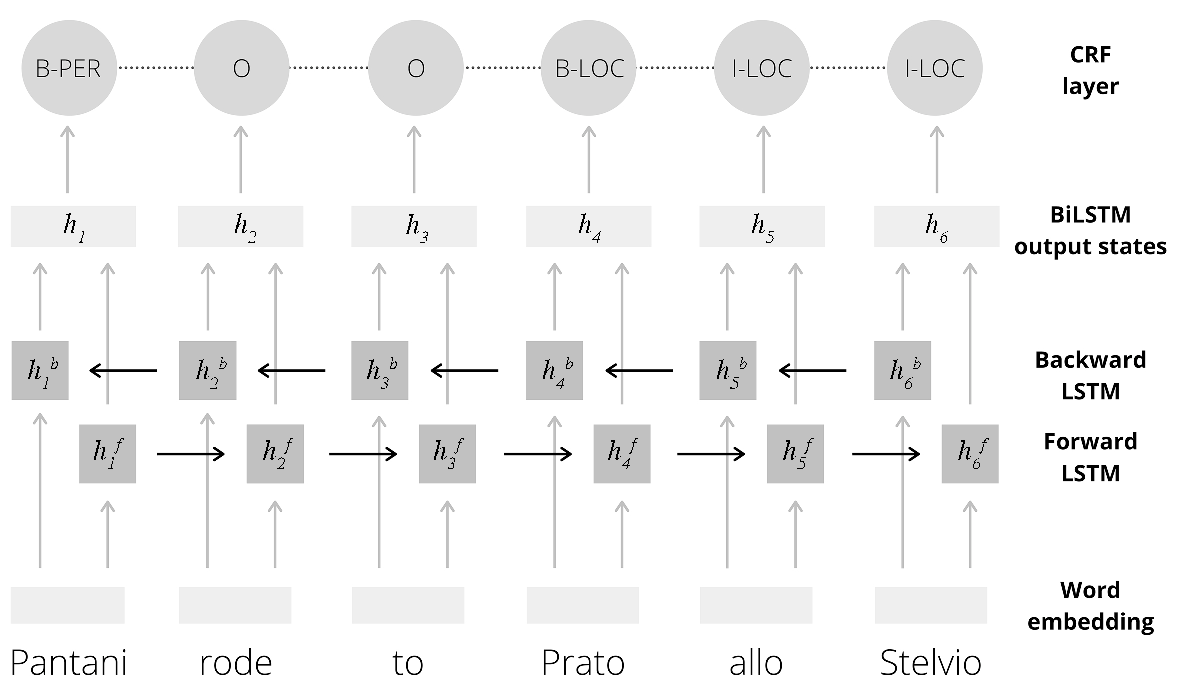
\includegraphics[width=1\linewidth]{images/bilstmcrf} 

}

\caption{A simplified representation of the BiLSTM-CRF architecture that was used to perform NER for the experiments reported in this thesis. The input of the BiLSTM are either static, task-specific or contextualized word embeddings (or a concatenation of different embedding types). The forward (\(\mathbf{h}_i^f\)) and backward (\(\mathbf{h}_i^b\)) output states of the BiLSTM are concatenated into a contextualized representation (\(\mathbf{h}_i = [\mathbf{h}_i^f; \mathbf{h}_i^b]\)) that is used to predict the correct tag sequence using a Conditional Random Field (CRF), as described in the text.}\label{fig:bilstmcrf}
\end{figure}

For the benchmark datasets (CoNLL2002, CoNLL2003, WikiNER), the model hyperparameters were based on the \href{https://github.com/flairNLP/flair/blob/master/resources/docs/EXPERIMENTS.md}{best known configuration} for the CoNLL tasks as reported by the authors of the \href{https://github.com/flairNLP/flair}{Flair library}. In what follows we provide the parameter names and their selected values of the \texttt{SequenceTagger} and \texttt{ModelTrainer} classes of the Flair library (unless default values were selected). The dimensionality of the BiLSTM-CRF hidden states (\texttt{hidden\_size}) was set equal to 256. Training was done using stochastic gradient descent with a \texttt{mini\_batch\_size} of 32 instances, i.e.~at each iteration, 32 sentences from the training set were propagated through the network (sentences were shuffled at each epoch). The initial \texttt{learning\_rate} was set to 0.1. Early stopping criteria were specified by setting \texttt{patience} = 3 and \texttt{anneal\_factor} = 0.5 which means that the learning rate was multiplied by a factor 0.5 when the validation F1-score did not improve for 3 consecutive epochs. When the learning rate dropped below the \texttt{min\_learning\_rate} of 0.0001 or after 100 epochs (as specified by the \texttt{max\_epochs} parameter), the training procedure was stopped. The final model was refitted on the training and validation set and performance was estimated through computing the micro-average precision, recall and F1-score (cf infra) on the held-out test set. The approach was similar for the Faktion datasets, with some minor changes in terms of the NER classifier architecture and the early stopping criteria to optimize performance for these datasets. The hyperparameters for both the benchmark and Faktion datasets are summarized in table \ref{tab:params}.

\begin{table}

\caption{\label{tab:params}Overview of the hyperparameter configuration for all NER experiments on the benchmark datasets and Faktion datasets. The terminology used here is consistent with the parameters of the \texttt{SequenceTagger} and \texttt{ModelTrainer} classes of the \href{https://github.com/flairNLP/flair}{Flair NLP library}. Further details can be found in the \href{https://github.com/flairNLP/flair/tree/master/resources/docs}{documentation of the Flair NLP library} or in the \href{https://github.com/arthur-arthur/NER/}{GitHub repository} of this thesis.}
\centering
\begin{tabular}[t]{lll}
\toprule
Parameter & Benchmark & Faktion\\
\midrule
hidden\_size & 256 & 32\\
learning\_rate & 0.1 & 0.1\\
anneal\_factor & 0.5 & 0.8\\
patience & 3 & 3\\
min\_learning\_rate & 1e-04 & 1e-04\\
\addlinespace
mini\_batch\_size & 32 & 8\\
max\_epochs & 100 & 100\\
\bottomrule
\end{tabular}
\end{table}



All models were trained using the cloud computational environment of \href{https://www.kaggle.com}{Kaggle}, either on a CPU (4 cores, 16 Gb RAM) or on a single NVIDIA Tesla P100 GPU (2 CPU cores, 16 Gb RAM) (Python 3.7.6). We made use of the Kaggle API to automatically configure Python scripts for each experiment and push it to the Kaggle environment from a simple command line interface. All code and information to reproduce the experiments can be found on the \href{https://github.com/arthur-arthur/NER}{Github repository (arthur-arthur/NER)} of this thesis.

\hypertarget{ner-evaluation}{%
\section{NER evaluation}\label{ner-evaluation}}

According to the \href{https://www.clips.uantwerpen.be/conll2000/chunking/output.html}{CoNLL guidelines}, evaluation of NER is performed at the entity-level, not at the token or word-level (to clarify this, an example is provided at the end of this paragraph). This has some consequences on the type of metrics that are used to evaluate NER performance, as well as on their interpretation.

Firstly, since entity-level evaluation is based on the sets of predicted and true entities, there is no clear definition of a ``true negative'' entity \citep{esuli2010}. Hence, evaluation metrics that are a function of the number of true negatives (ROC analysis, classification accuracy, Matthews Correlation Coefficient,\ldots{}) are not very meaningful in this context. For this reason, NER performance is commonly evaluated in terms of entity-level precision, recall and F1-score. Precision gives the proportion of all predicted entities that are indeed correct:

\[
P = \frac{TP}{TP + FP}
\]
with TP and FP being true positives and false positives, respectively. Recall indicates how much of the entities in the dataset were correctly predicted:

\[
R = \frac{TP}{TP + FN}
\]
with FN being false negatives. Note that one can easily design a system that achieves high recall by predicting all instances as entities such that \(FN=0\). This will typically result in a high number of false positives and, hence, a low precision. Conversely, when only a single entity from the entire dataset is correctly predicted, \(P=1\). In that case, the number of false negatives is typically high and, hence, recall will be low. The goal is therefore to find a system that has an optimal balance between precision and recall, which is commonly expressed in terms of the F1-score - the gold standard evaluation metric for NER \citep{tjongkimsang2003}. The F1-score is defined as the harmonic mean of precision and recall:

\[
F_1 = \frac{2PR}{P + R}
\]

To illustrate how gold standard entity-level evaluation of NER systems is performed, we provide the following example sentence (for simplicity, the example includes only a single entity class, this extends naturally to cases with multiple classes):

\begin{itemize}
\tightlist
\item
  \textbf{Gold sentence: }\\
  ``From Bormio {[}B-LOC{]} to Prato {[}B-LOC{]} allo {[}I-LOC{]} Stelvio {[}I-LOC{]}''.
\item
  \textbf{Predicted sentence: }\\
  ``From Bormio {[}B-LOC{]} to Prato {[}B-LOC{]} allo Stelvio {[}B-LOC{]}''
\end{itemize}

The set of true entities thus includes two instances: ``Bormio'' and ``Prato allo Stelvio''. The NER system correctly identified the token ``Bormio'' as a location, i.e.~this is a true positive (TP) prediction. The system failed to correctly predict the segment ``Prato allo Stelvio'' as a location spanning three tokens, i.e.~this is a false negative (FN) prediction. In addition, the NER tagger predicted ``Prato {[}B-LOC{]}'' and ``Stelvio {[}B-LOC{]}'' as two separate entities, while these were not in the set of true entities. Hence, these are two false positive (FP) predictions. Overall, the precision for this example is \(\frac{1}{1+2} = 0.33\), the recall is \(\frac{1}{1 + 1} = 0.5\) and the F1-score is \(\frac{2 \times 0.33 \times 0.50}{0.33 + 0.50} = 0.40\).

When there are multiple entity classes to predict (which is the case for most NER systems), the overall performance of the system can be expressed in terms of the macro-average or micro-average precision, recall or F1-scores. Macro-averaging involves simply averaging the scores per entity class, while the micro-average refers to the weighted average of the class scores, with the weights being determined by the number of instances per class. Since the latter takes the class balance into account. NER performance is typically evaluated and reported in terms of the micro-average F1-score. We will adhere to this convention and report the micro-average precision, recall and F1-scores for the NER experiments performed during this thesis. For the benchmark datasets, only a single training run was performed. When multiple training runs were performed (i.e.~for the Faktion datasets), the F1-scores were reported as mean ± standard error of the mean (sem) for \(k = 5\) runs. All scores reported in this thesis were computed on the held-out test set.

\hypertarget{results}{%
\chapter{Results}\label{results}}

\hypertarget{benchmark-datasets-1}{%
\section{Benchmark datasets}\label{benchmark-datasets-1}}

\hypertarget{conll2003---english}{%
\subsection{CoNLL2003 - English}\label{conll2003---english}}

The best results obtained on the CoNLL2003 task (Figure \ref{fig:conll2003-fig}) using state-of-the-art contextualized embeddings from pretrained LMs were similar to the state-of-the-art results reported in literature (Table \ref{tab:conll2003-tab}). As a proof of concept to demonstrate the added value of ``transfer learning'' in the context of NER, the BiLSTM-CRF classifier was trained without any input from pretrained (either static or contextualized) embeddings, i.e.~only using randomly initialized embeddings that were updated during training to minimize the loss w.r.t. to the NER objective. Both the OHE and character-feature embeddings performed poorly, with F1-scores of 74.0 \% and 75.4 \%, respectively (Figure \ref{fig:conll2003-fig}). Performance improved drastically when using static BytePair embeddings alone (Figure \ref{fig:conll2003-fig}), or when all static and task-specific embeddings were concatenated into a single vector. However, as expected, best performance was provided with contextualized representations from pretrained LMs like BERT, Flair or both (Table \ref{tab:conll2003-tab}). Even though the additional increase in performance from concatenating these contextualized representations with static and task-specific embeddings was small, this trend was consistent for both monolingual and multilingual embeddings.

While the monolingual embeddings appeared to outperform the multilingual embeddings, the differences between large stackings of respectively BERT and mBERT embeddings were surprisingly small (F1-scores of 92.1 \% vs.~91.4 \%, respectively), with mBERT-based embeddings being clearly superior to mFlair-based embeddings (Table \ref{tab:conll2003-tab}).

\begin{figure}

{\centering 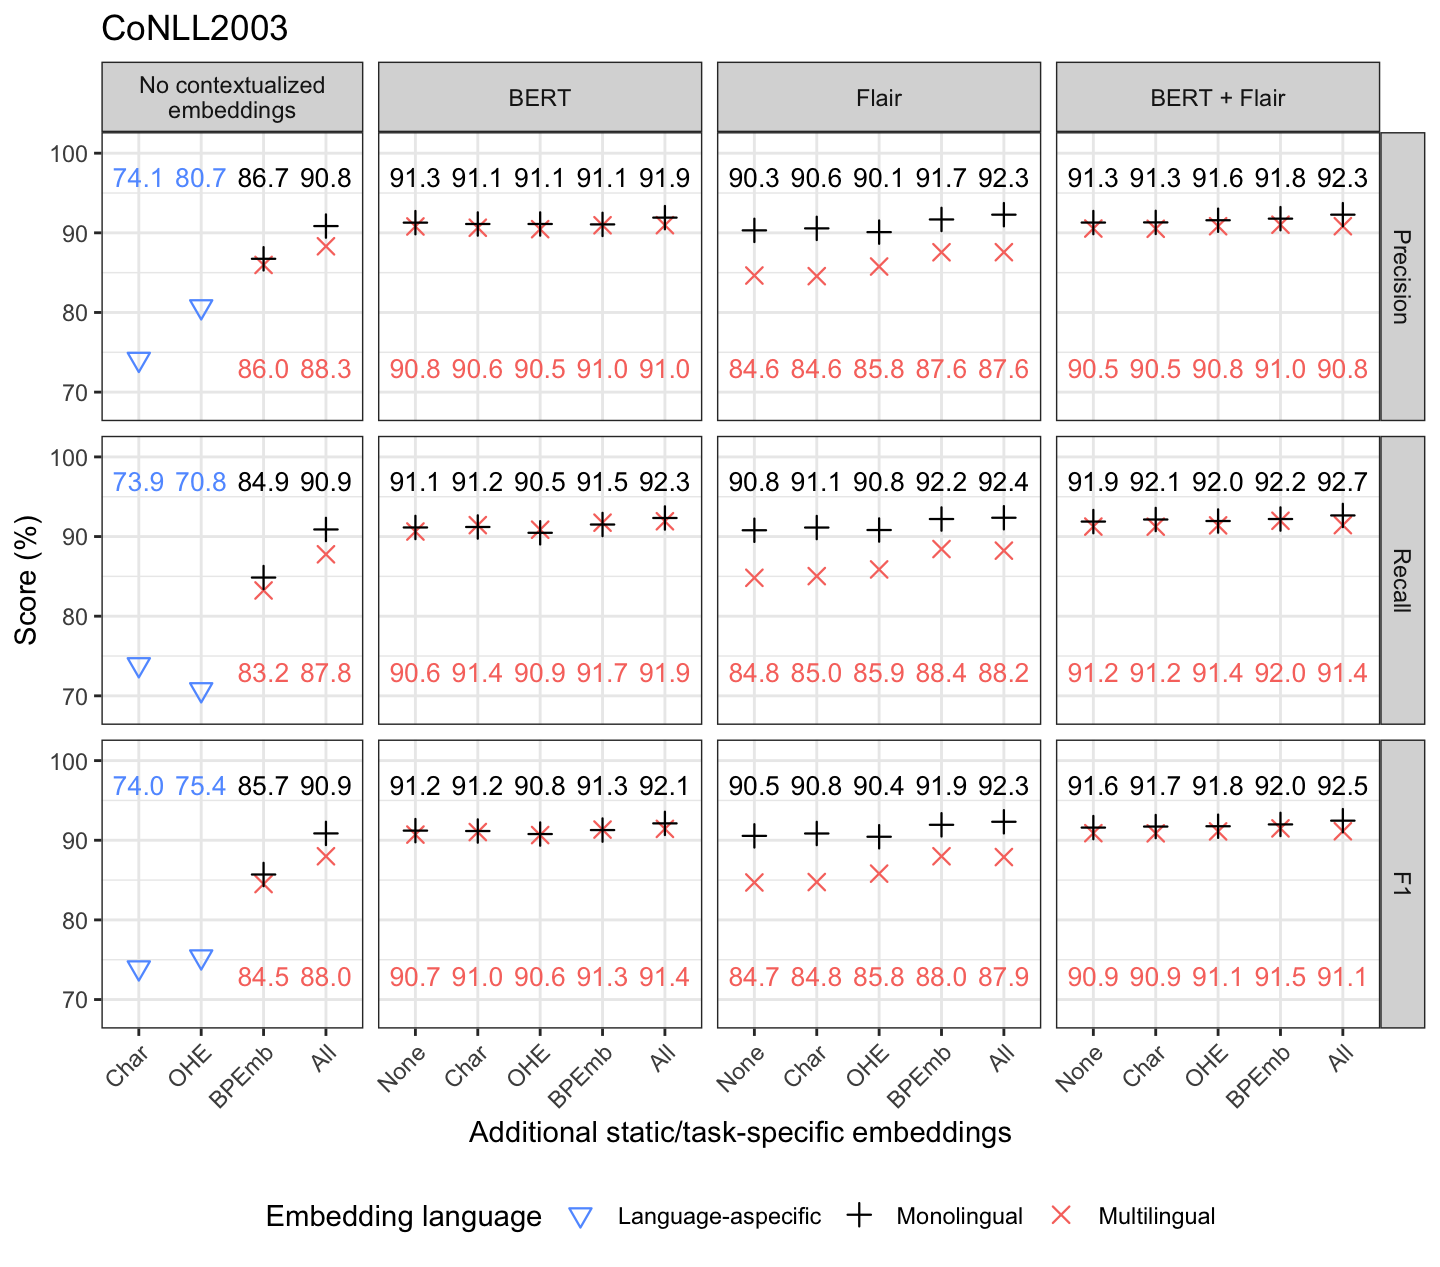
\includegraphics{Thesis_Arthur_Leloup_files/figure-latex/conll2003-fig-1} 

}

\caption{Test-set micro-average precision (top), recall (middle) and F1-scores (bottom) for the English CoNLL2003 task. The results are grouped according to the constituents of each (stacked) embedding, consistent with Table \ref{tab:embeddings}. The contextualized embedding type, if present, is indicated on the different panels from left to right. The stacked/task-specific embedding type (if present) is shown on the x-axis. The scores for every monolingual or multilingual model are indicated in the upper and lower region of each panel, respectively. \emph{BERT: BERT (monolingual) or mBERT (multilingual); Flair: Flair (monolingual) or mFlair (multilingual); Char: character embeddings; OHE: One Hot Embeddings; BPEmb: BytePair embeddings (English/multilingual); All: concatenation of all static and task-specific embeddings, i.e. {[}Char + OHE + BPEmb + fastText{]} (for monolingual embeddings) or {[}Char + OHE + mBPEmb{]} (for multilingual embeddings).}}\label{fig:conll2003-fig}
\end{figure}



\begin{table}

\caption{\label{tab:conll2003-tab}Results acquired on the English CoNLL2003 task with monolingual and multilingual NER systems. The results for the best-performing model for the original CoNLL2003 shared task is included for comparison \citep{florian2003}. A complete overview of all results is provided in Table \ref{tab:apx-en}.}
\centering
\begin{tabular}[t]{llll}
\toprule
Description & Precision & Recall & F1-score\\
\midrule
\addlinespace[0.3em]
\multicolumn{4}{l}{\textbf{Monolingual}}\\
\textcolor[HTML]{999999}{\hspace{1em}CoNLL2003 best - IBM Florian \textsuperscript{a}} & \textcolor[HTML]{999999}{89.0} & \textcolor[HTML]{999999}{88.5} & \textcolor[HTML]{999999}{88.7}\\
\textcolor[HTML]{999999}{\hspace{1em}Flair - BiLSTM-CRF \textsuperscript{b}} & \textcolor[HTML]{999999}{} & \textcolor[HTML]{999999}{} & \textcolor[HTML]{999999}{93.1}\\
\textcolor[HTML]{999999}{\hspace{1em}BERT base - finetuned \textsuperscript{c}} & \textcolor[HTML]{999999}{} & \textcolor[HTML]{999999}{} & \textcolor[HTML]{999999}{92.4}\\
\hspace{1em}[all]: fastT + BPEmb + Char + OHE & 90.8 & 90.9 & 90.9\\
\hspace{1em}BERT & 91.3 & 91.1 & 91.2\\
\hspace{1em}BERT + [all] & 91.9 & 92.3 & 92.1\\
\hspace{1em}Flair & 90.3 & 90.8 & 90.5\\
\hspace{1em}Flair + [all] & 92.3 & 92.4 & 92.3\\
\hspace{1em}BERT + Flair & 91.3 & 91.9 & 91.6\\
\hspace{1em}BERT + Flair + [all] & 92.3 & 92.7 & \textbf{92.5}\\
\addlinespace[0.3em]
\multicolumn{4}{l}{\textbf{Multilingual}}\\
\textcolor[HTML]{999999}{\hspace{1em}mBERT - finetuned \textsuperscript{d}} & \textcolor[HTML]{999999}{} & \textcolor[HTML]{999999}{} & \textcolor[HTML]{999999}{92.0}\\
\hspace{1em}[all]: mBPEmb + Char + OHE & 88.3 & 87.8 & 88.0\\
\hspace{1em}mBERT & 90.8 & 90.6 & 90.7\\
\hspace{1em}mBERT + [all] & 91.0 & 91.9 & \textbf{91.4}\\
\hspace{1em}mFlair & 84.6 & 84.8 & 84.7\\
\hspace{1em}mFlair + [all] & 87.6 & 88.2 & 87.9\\
\hspace{1em}mBERT + mFlair & 90.5 & 91.2 & 90.9\\
\hspace{1em}mBERT + mFlair + [all] & 90.8 & 91.4 & 91.1\\
\bottomrule
\multicolumn{4}{l}{\textit{References}}\\
\multicolumn{4}{l}{\textsuperscript{a} Florian et al (2003)}\\
\multicolumn{4}{l}{\textsuperscript{b} Akbik et al (2018)}\\
\multicolumn{4}{l}{\textsuperscript{c} Devlin et al (2019)}\\
\multicolumn{4}{l}{\textsuperscript{d} Wu et al (2019)}\\
\end{tabular}
\end{table}



\hypertarget{conll2002---dutch}{%
\subsection{CoNLL2002 - Dutch}\label{conll2002---dutch}}

Results were similar for the Dutch CoNLL2002 task (Figure \ref{fig:conll2002-fig}, Table \ref{tab:conll2002-tab}) in the sense that task-specific representations (i.e.~character embeddings (F1: 67.8 \%) or OHE (F1: 61.7 \%)) were clearly inferior to embeddings obtained from pretrained LMs, with the best-performing monolingual system being based on the large (i.e.~5614-dimensional) concatenations of embeddings from both BERTje and Dutch Flair embeddings, stacked with Dutch fastText, Dutch BytePair and task-specific OHE and character embeddings (F1: 93.0 \%, Table \ref{tab:conll2002-tab}). Even though this is the result of only a single training run, all the monolingual embeddings based on BERTje consistently outperformed the result reported in the BERTje paper itself (F1: 90.2 \%) \citep{devries2019} as well as the current best result on the CoNLL2002 task, obtained by the fine-tuned mBERT model (F1-score: 90.9 \%) \citep{wu2019}. In contrast to the English CoNLL2003 task, monolingual embeddings from the Flair model performed poorly as compared to the BERT-based embeddings, with this difference being particularly pronounced for the multilingual embeddings (Table \ref{tab:conll2002-tab}).

\begin{figure}

{\centering 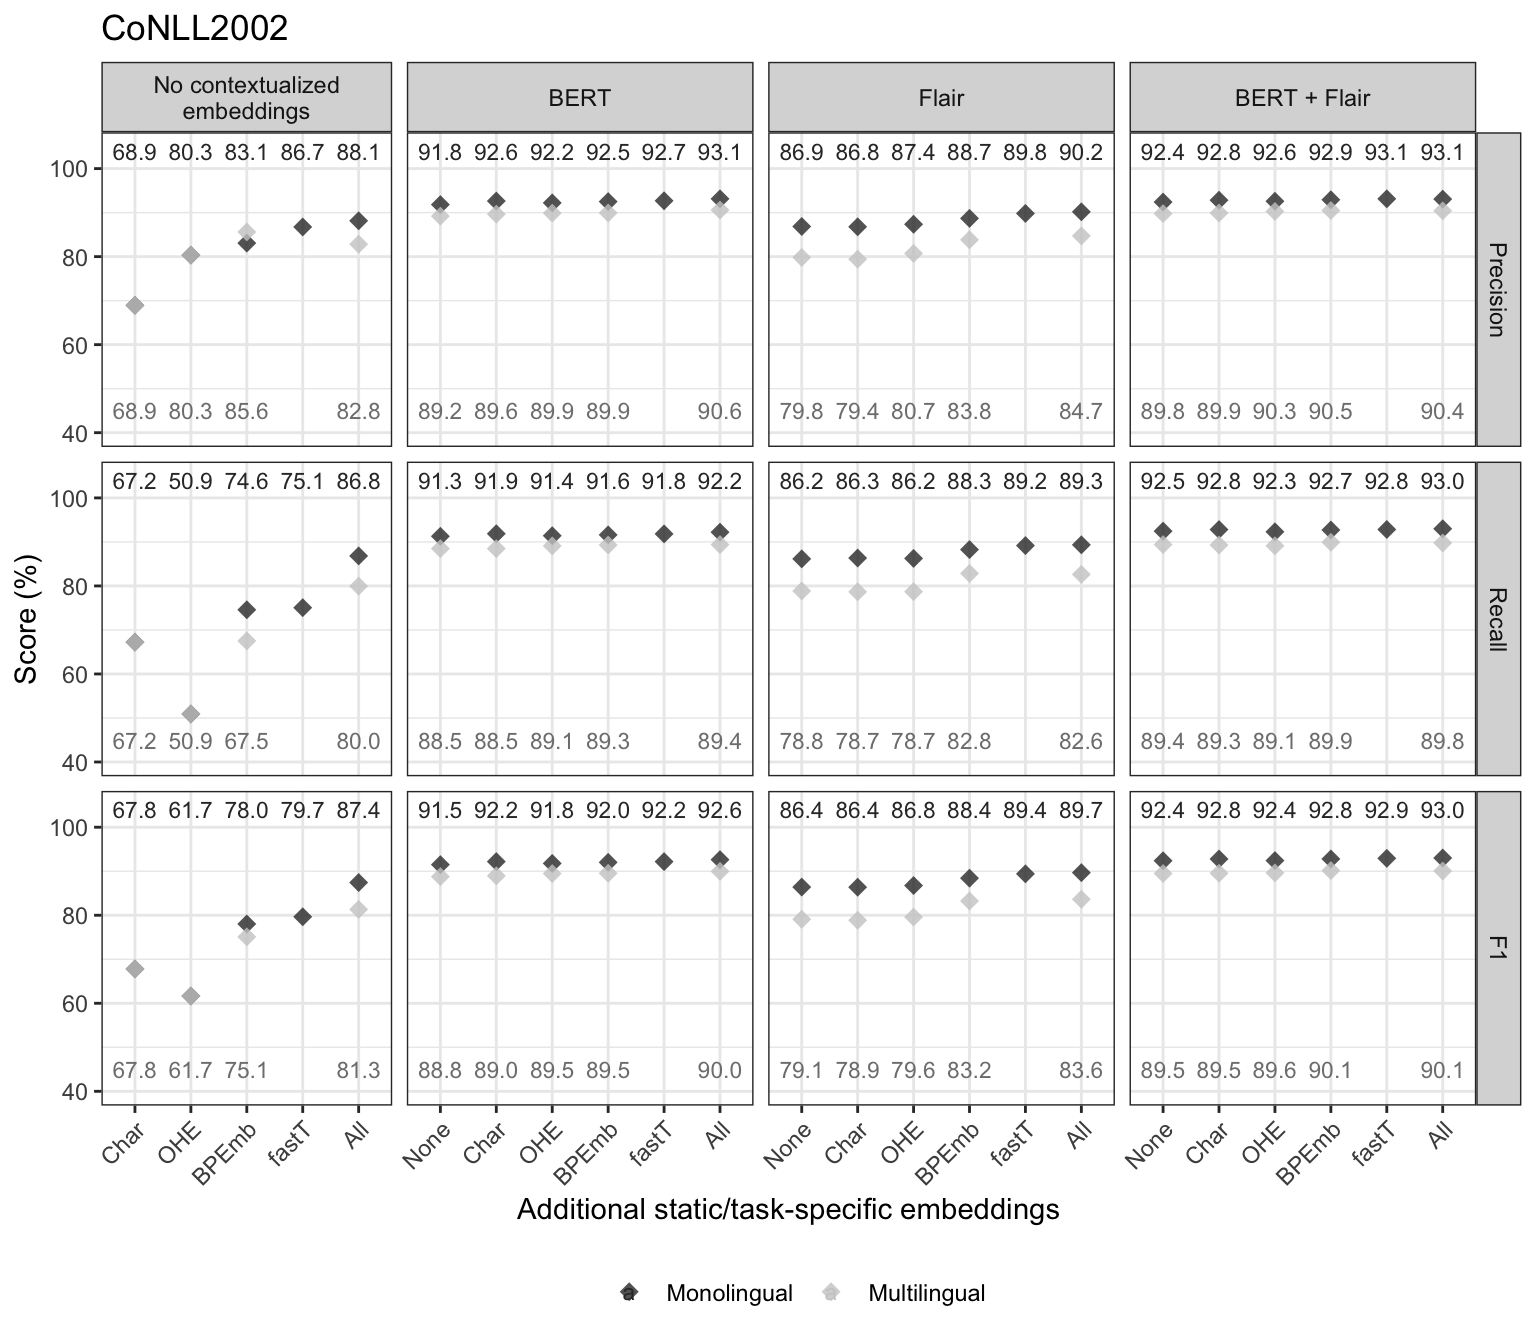
\includegraphics{Thesis_Arthur_Leloup_files/figure-latex/conll2002-fig-1} 

}

\caption{Test-set micro-average precision (top), recall (middle) and F1-scores (bottom) for the Dutch CoNLL2002 task. The results are grouped according to the constituents of each (stacked) embedding, consistent with Table \ref{tab:embeddings}. The contextualized embedding type, if present, is indicated on the different panels from left to right. The stacked/task-specific embedding type (if present) is shown on the x-axis. The scores for every monolingual or multilingual model are indicated in the upper and lower region of each panel, respectively. \emph{BERT: BERTje (monolingual) or mBERT (multilingual); Flair: Flair Nl (monolingual) or mFlair (multilingual); Char: character embeddings; OHE: One Hot Embeddings; BPEmb: BytePair embeddings (Dutch/multilingual); All: concatenation of all static and task-specific embeddings, i.e. {[}Char + OHE + BPEmb + fastText{]} (for monolingual embeddings) or {[}Char + OHE + mBPEmb{]} (for multilingual embeddings).}}\label{fig:conll2002-fig}
\end{figure}



\begin{table}

\caption{\label{tab:conll2002-tab}Results acquired on the Dutch CoNLL2002 task with monolingual and multilingual NER systems. The best-performing model for the original CoNLL2002 shared task \citep{carreras2002} is included for comparison. A complete overview of all results is provided in Table \ref{tab:apx-nl}.}
\centering
\begin{tabular}[t]{llll}
\toprule
Description & Precision & Recall & F1-score\\
\midrule
\addlinespace[0.3em]
\multicolumn{4}{l}{\textbf{Monolingual}}\\
\textcolor[HTML]{999999}{\hspace{1em}CoNLL2002 best - AdaBoost \textsuperscript{a}} & \textcolor[HTML]{999999}{77.8} & \textcolor[HTML]{999999}{76.3} & \textcolor[HTML]{999999}{77.1}\\
\textcolor[HTML]{999999}{\hspace{1em}Flair NL - BiLSTM-CRF \textsuperscript{b}} & \textcolor[HTML]{999999}{} & \textcolor[HTML]{999999}{} & \textcolor[HTML]{999999}{89.6}\\
\textcolor[HTML]{999999}{\hspace{1em}fine-tuned BERTje \textsuperscript{c}} & \textcolor[HTML]{999999}{} & \textcolor[HTML]{999999}{} & \textcolor[HTML]{999999}{90.2}\\
\hspace{1em}[all]: fastT + BPEmb + Char + OHE & 88.1 & 86.8 & 87.4\\
\hspace{1em}BERTje & 91.8 & 91.3 & 91.5\\
\hspace{1em}BERTje + [all] & 93.1 & 92.2 & 92.6\\
\hspace{1em}Flair & 86.9 & 86.2 & 86.4\\
\hspace{1em}Flair + [all] & 90.2 & 89.3 & 89.7\\
\hspace{1em}BERTje + Flair & 92.4 & 92.5 & 92.4\\
\hspace{1em}BERTje + Flair + [all] & 93.1 & 93.0 & \textbf{93.0}\\
\addlinespace[0.3em]
\multicolumn{4}{l}{\textbf{Multilingual}}\\
\textcolor[HTML]{999999}{\hspace{1em}fine-tuned mBERT \textsuperscript{d}} & \textcolor[HTML]{999999}{} & \textcolor[HTML]{999999}{} & \textcolor[HTML]{999999}{90.9}\\
\hspace{1em}[all]: mBPEmb + Char + OHE & 82.8 & 80.0 & 81.3\\
\hspace{1em}mBERT & 89.2 & 88.5 & 88.8\\
\hspace{1em}mBERT + [all] & 90.6 & 89.4 & 90.0\\
\hspace{1em}mFlair & 79.8 & 78.8 & 79.1\\
\hspace{1em}mFlair + [all] & 84.7 & 82.6 & 83.6\\
\hspace{1em}mBERT + mFlair & 89.8 & 89.4 & 89.5\\
\hspace{1em}mBERT + mFlair + [all] & 90.4 & 89.8 & \textbf{90.1}\\
\bottomrule
\multicolumn{4}{l}{\textit{References}}\\
\multicolumn{4}{l}{\textsuperscript{a} Carreras et al 2002}\\
\multicolumn{4}{l}{\textsuperscript{b} GitHub: stefan-it/flair-experiments}\\
\multicolumn{4}{l}{\textsuperscript{c} GitHub: wietsedv/bertje}\\
\multicolumn{4}{l}{\textsuperscript{d} Wu et al (2019)}\\
\end{tabular}
\end{table}



\hypertarget{wikiner---french}{%
\subsection{WikiNER - French}\label{wikiner---french}}

To evaluate how monolingual and multilingual embeddings performed on a French NER task, we used a small subset of the French WikiNER dataset. Even though the entity classes (i.e.~PER, ORG, LOC and MISC) were identical to the CoNLL2002 and CoNLL2003 datasets, performance was - on average - lower for the WikiNER dataset. However, the general trend that stacking multiple embedding types together typically improves performance was also observed here (Figure \ref{fig:wikiner-fig}). This was less pronounced for monolingual embeddings based on CamemBERT or multilingual embeddings based on mBERT, where performance was already relatively high at baseline (i.e.~when no additional static or task-specific embeddings were included) (Table \ref{tab:conll2002-tab}).

In general - for all three monolingual datasets - high-dimensional vectors based on contextualized representations obtained from pretrained LMs clearly improved performance as compared to high-dimensional stackings of static and task-specific representations alone. BERT-based embeddings generally outperformed Flair-based embeddings, except for monolingual English NER, where Flair- and BERT-based embeddings performed similarly.

\begin{figure}

{\centering 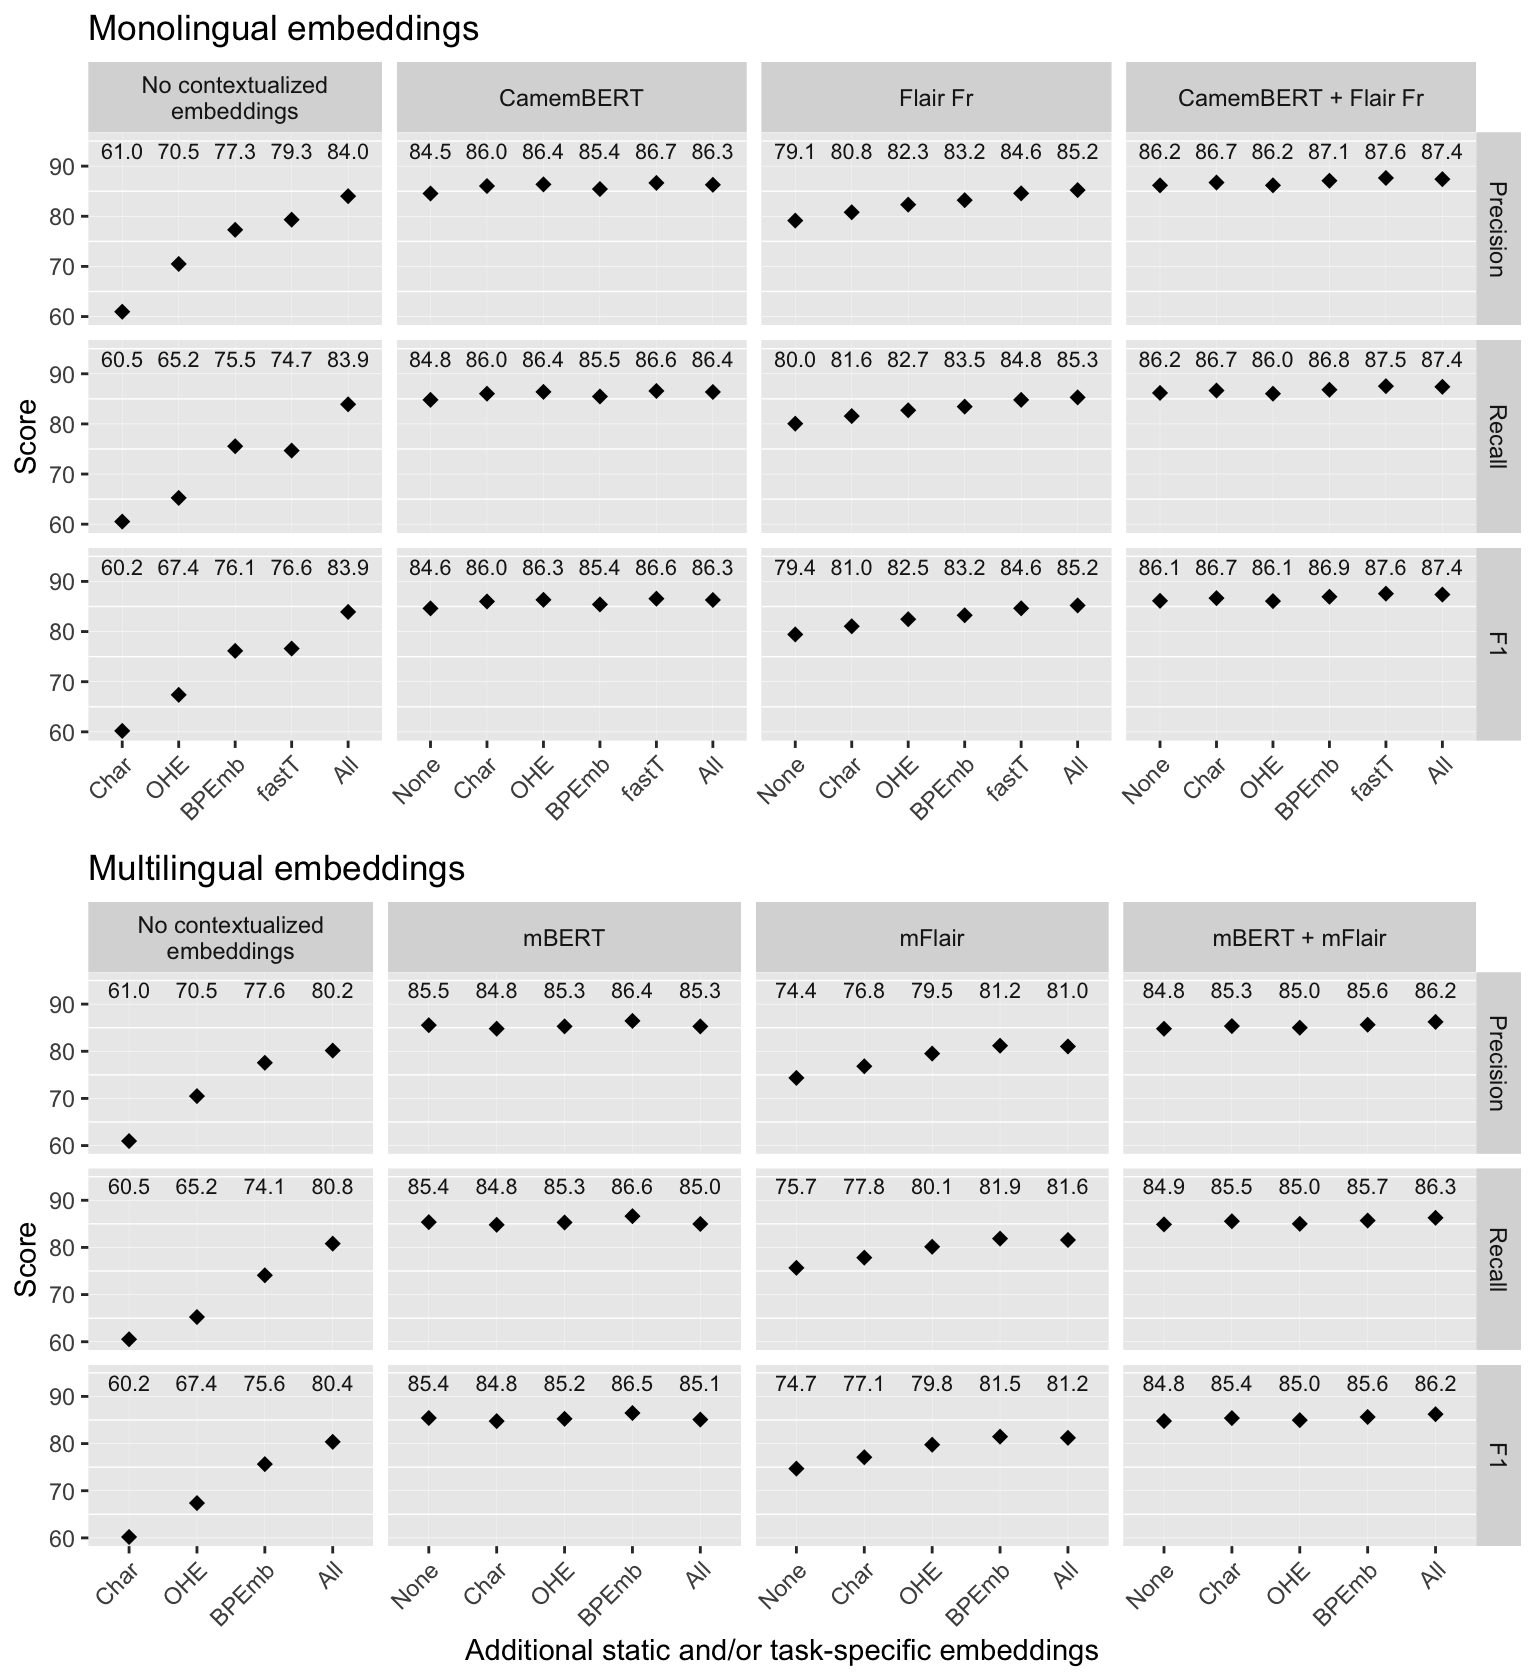
\includegraphics{Thesis_Arthur_Leloup_files/figure-latex/wikiner-fig-1} 

}

\caption{Test-set micro-average precision (top), recall (middle) and F1-scores (bottom) for the French WikiNER task. The results are grouped according to the constituents of each (stacked) embedding, consistent with Table \ref{tab:embeddings}. The contextualized embedding type, if present, is indicated on the different panels from left to right. The stacked/task-specific embedding type (if present) is shown on the x-axis. The scores for every monolingual or multilingual model are indicated in the upper and lower region of each panel, respectively. \emph{BERT: CamemBERT (monolingual) or mBERT (multilingual); Flair: Flair Fr (monolingual) or mFlair (multilingual); Char: character embeddings; OHE: One Hot Embeddings; BPEmb: BytePair embeddings (French/multilingual); All: concatenation of all static and task-specific embeddings, i.e. {[}Char + OHE + BPEmb + fastText{]} (for monolingual embeddings) or {[}Char + OHE + mBPEmb{]} (for multilingual embeddings).}}\label{fig:wikiner-fig}
\end{figure}



\begin{table}

\caption{\label{tab:wikiner-tab}Overview of results acquired on the French WikiNER task with monolingual and multilingual NER systems. Note that we used a subset consisting of only 10 \% of the entire WikiNER dataset. A complete overview of all results is provided in Table \ref{tab:apx-fr}.}
\centering
\begin{tabular}[t]{llll}
\toprule
Description & Precision & Recall & F1-score\\
\midrule
\addlinespace[0.3em]
\multicolumn{4}{l}{\textbf{Monolingual}}\\
\textcolor[HTML]{999999}{\hspace{1em}SpaCy fr \textsuperscript{a}} & \textcolor[HTML]{999999}{82.2} & \textcolor[HTML]{999999}{81.6} & \textcolor[HTML]{999999}{81.9}\\
\textcolor[HTML]{999999}{\hspace{1em}Flair \textsuperscript{b}} & \textcolor[HTML]{999999}{87.9} & \textcolor[HTML]{999999}{87.7} & \textcolor[HTML]{999999}{87.8}\\
\hspace{1em}[all]: fastT + BPEmb + Char + OHE & 84.0 & 83.9 & 83.9\\
\hspace{1em}CamemBERT & 84.5 & 84.8 & 84.6\\
\hspace{1em}CamemBERT + [all] & 86.3 & 86.4 & 86.3\\
\hspace{1em}Flair & 79.1 & 80.0 & 79.4\\
\hspace{1em}Flair + [all] & 85.2 & 85.3 & 85.2\\
\hspace{1em}CamemBERT + Flair & 86.2 & 86.2 & 86.1\\
\hspace{1em}CamemBERT + Flair + [all] & 87.4 & 87.4 & \textbf{87.4}\\
\addlinespace[0.3em]
\multicolumn{4}{l}{\textbf{Multilingual}}\\
\textcolor[HTML]{999999}{\hspace{1em}SpaCy XX \textsuperscript{c}} & \textcolor[HTML]{999999}{80.3} & \textcolor[HTML]{999999}{79.5} & \textcolor[HTML]{999999}{79.9}\\
\hspace{1em}[all]: mBPEmb + Char + OHE & 80.2 & 80.8 & 80.4\\
\hspace{1em}mBERT & 85.5 & 85.4 & 85.4\\
\hspace{1em}mBERT + [all] & 85.3 & 85.0 & 85.1\\
\hspace{1em}mFlair & 74.4 & 75.7 & 74.7\\
\hspace{1em}mFlair + [all] & 81.0 & 81.6 & 81.2\\
\hspace{1em}mBERT + mFlair & 84.8 & 84.9 & 84.8\\
\hspace{1em}mBERT + mFlair + [all] & 86.2 & 86.3 & \textbf{86.2}\\
\bottomrule
\multicolumn{4}{l}{\textit{References}}\\
\multicolumn{4}{l}{\textsuperscript{a} GitHub: flairNLP/flair/issues/238}\\
\multicolumn{4}{l}{\textsuperscript{b} GitHub: flairNLP/flair/issues/238}\\
\multicolumn{4}{l}{\textsuperscript{c} spacy.io/models/xx}\\
\end{tabular}
\end{table}



\hypertarget{trilingual-ner}{%
\subsection{Trilingual NER}\label{trilingual-ner}}

The aforementioned results support our first research hypothesis that monolingual embeddings outperform multilingual embeddings in the case of multilingual input data, which might reflect the lack of language-specific knowledge of the multilingual embeddings. The difference, however, was small for multilingual representations based on mBERT embeddings. To test the hypothesis that the multilingual knowledge acquired by mBERT during pretraining is particularly beneficial when the input data is multilingual, we combined random subsets of the CoNLL2002, CoNLL2003 and WikiNER dataset into a single, multilingual dataset. We evaluated NER performance using all monolingual and multilingual embeddings used for the monolingual NER tasks. Evaluating the different monolingual embeddings on the multilingual dataset provides an indication on how NER performance might suffer from incorrect predictions by an upstream language-prediction system in a document annotation pipeline like Metamaze (cf supra).

The results for the Dutch monolingual embeddings and the different multilingual embeddings on the trilingual benchmark dataset are visualized in Figure \ref{fig:trilingual-fig}. Task-specific representations (OHE and Character embeddings) performed, again, poorly, with F1-scores of 60.4 \% and 60.8 \%, respectively (Table \ref{tab:apx-trired}). Interestingly, adding contextualized embeddings from pretrained LMs improved results drastically (Table \ref{tab:benchmark-multi-tab}), again demonstrating that the acquired knowledge of the LM provided representations that encoded information highly relevant for the NER classifier to perform well - even when this LM was trained in the language that represented merely one third of the entire dataset.

For all monolingual embeddings, concatenating both Flair and BERT embeddings together improved performance as compared to the representations obtained from either Flair- or BERT-based embeddings alone (Table \ref{tab:benchmark-multi-tab}). When increasing the dimensionality of the BERT + Flair stacked embeddings further through concatenating fastText and BytePair embeddings (in the respective languages) and task-specific OHE and character embeddings, performance increased further to roughly 85 \% for all monolingual systems (Table \ref{tab:apx-trired}). Interestingly, even mBERT embeddings alone performed better on this multilingual dataset (F1-score: 86.5 \%), supporting our second research hypothesis that pretraining on a multilingual dataset improves performance for multilingual NER as compared to the monolingual LMs. An additional (slight) performance increase was achieved through stacking mBERT embeddings with mBytePair, OHE and character embeddings (F1-score: 87.5 \%) (Table \ref{tab:benchmark-multi-tab}). The performance of mFlair-based embeddings was again low, in general. Not only compared to mBERT-based embeddings, but even compared to monolingual embeddings containing no BERT- or Flair-based embeddings at all (Figure \ref{fig:trilingual-fig}).

\begin{figure}

{\centering 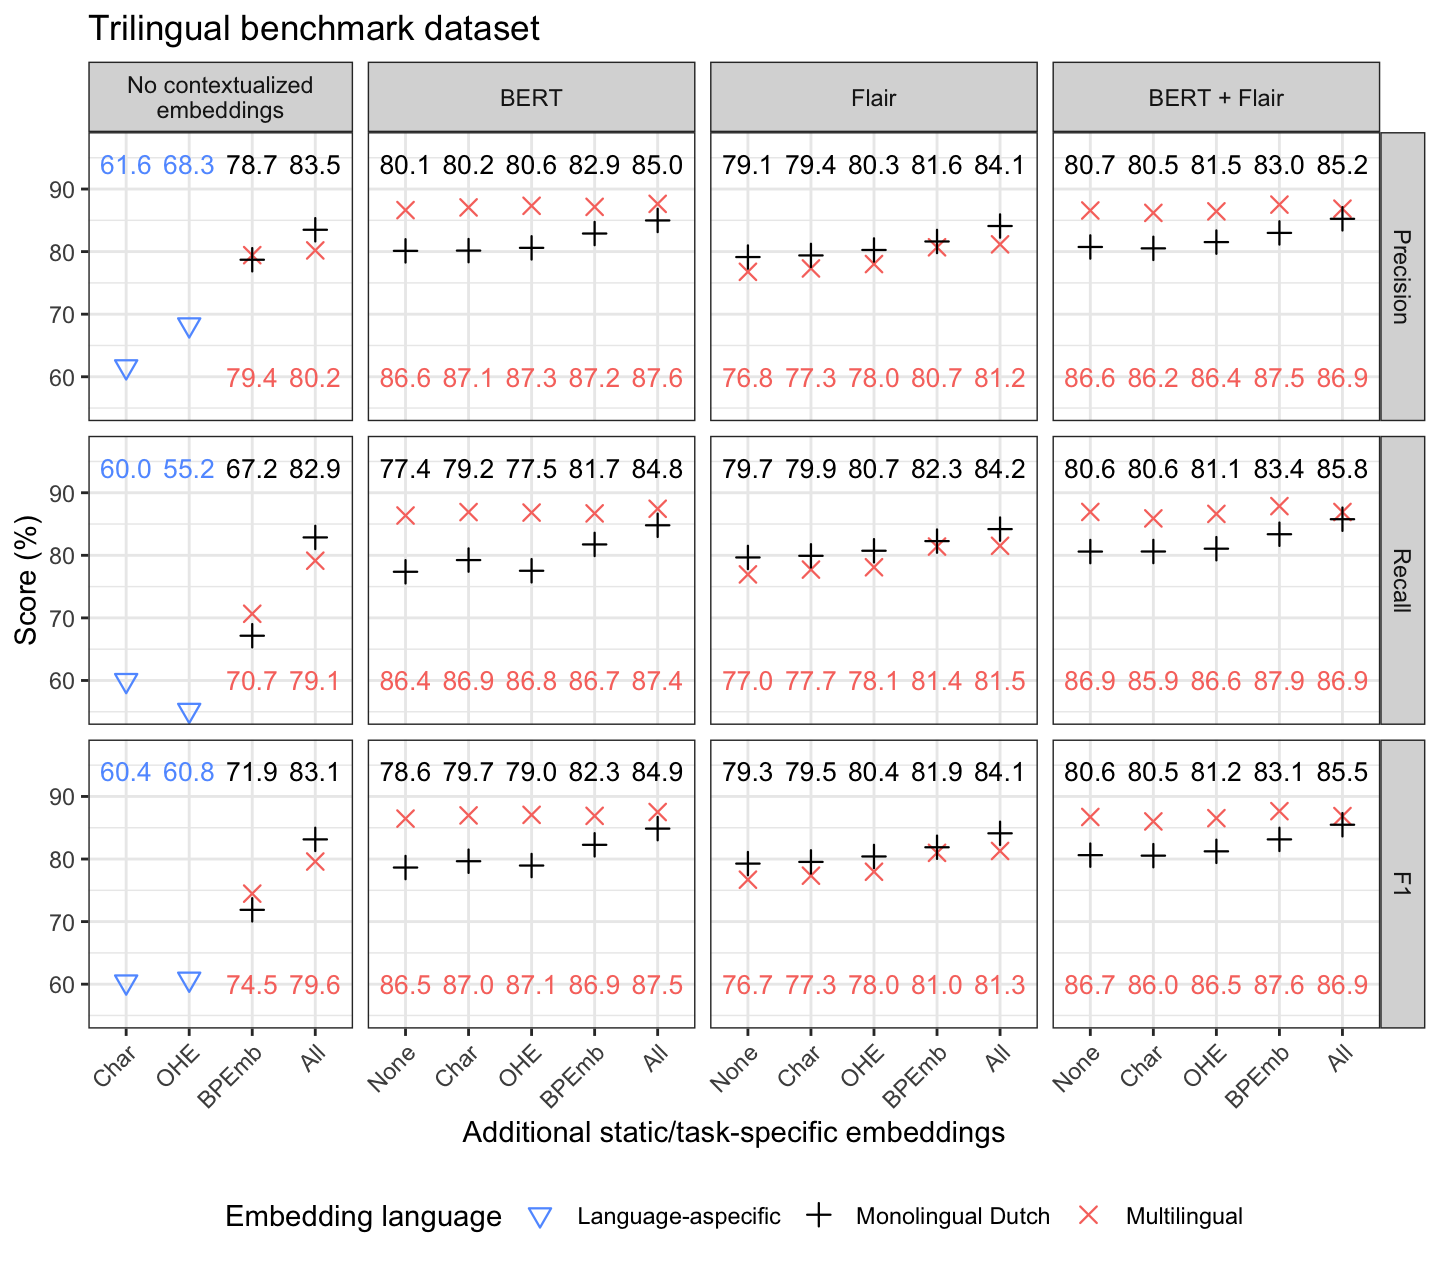
\includegraphics{Thesis_Arthur_Leloup_files/figure-latex/trilingual-fig-1} 

}

\caption{Test-set micro-average precision (top), recall (top) and F1-scores (top) for the multilingual (English + Dutch + French) benchmark dataset. The results are grouped according to the constituents of each (stacked) embedding, consistent with Table \ref{tab:embeddings}. The contextualized embedding type, if present, is indicated on the different panels from left to right. The stacked/task-specific embedding type (if present) is shown on the x-axis. For clarity, the results for the French and English embeddings are omitted. The scores for every monolingual or multilingual model are indicated in the upper and lower region of each panel, respectively. \emph{BERT: BERTje (monolingual) or mBERT (multilingual); Flair: Flair Nl (monolingual) or mFlair (multilingual); Char: character embeddings; OHE: One Hot Embeddings; BPEmb: BytePair embeddings (Dutch/multilingual); All: concatenation of all static and task-specific embeddings, i.e. {[}Char + OHE + BPEmb + fastText{]} (for monolingual embeddings) or {[}Char + OHE + mBPEmb{]} (for multilingual embeddings).}}\label{fig:trilingual-fig}
\end{figure}



\begin{table}

\caption{\label{tab:benchmark-multi-tab}Results obtained on the multilingual dataset, consisting of a random sample of the aformentioned English, Dutch and French benchmark datasets. A complete overview of all results is provided in Table \ref{tab:apx-trired}.}
\centering
\begin{tabular}[t]{llll}
\toprule
Embedding type & Precision & Recall & F1-score\\
\midrule
\addlinespace[0.3em]
\multicolumn{4}{l}{\textbf{Monolingual English embeddings}}\\
\hspace{1em}[all]: fastT + BPEmb + Char + OHE & 84.4 & 83.8 & 84.0\\
\hspace{1em}BERT & 82.0 & 81.0 & 81.4\\
\hspace{1em}BERT + [all] & 85.0 & 84.2 & 84.6\\
\hspace{1em}Flair & 79.5 & 79.2 & 79.2\\
\hspace{1em}Flair + [all] & 85.2 & 85.1 & 85.1\\
\hspace{1em}BERT + Flair & 83.5 & 83.4 & 83.4\\
\hspace{1em}BERT + Flair + [all] & 85.3 & 85.1 & \textbf{85.2}\\
\addlinespace[0.3em]
\multicolumn{4}{l}{\textbf{Monolingual Dutch embeddings}}\\
\hspace{1em}[all]: fastT + BPEmb + Char + OHE & 83.5 & 82.9 & 83.1\\
\hspace{1em}BERTje & 80.1 & 77.4 & 78.6\\
\hspace{1em}BERTje + [all] & 85.0 & 84.8 & 84.9\\
\hspace{1em}Flair & 79.1 & 79.7 & 79.3\\
\hspace{1em}Flair + [all] & 84.1 & 84.2 & 84.1\\
\hspace{1em}BERTje + Flair & 80.7 & 80.6 & 80.6\\
\hspace{1em}BERTje + Flair + [all] & 85.2 & 85.8 & \textbf{85.5}\\
\addlinespace[0.3em]
\multicolumn{4}{l}{\textbf{Monolingual French embeddings}}\\
\hspace{1em}[all]: fastT + BPEmb + Char + OHE & 83.8 & 83.0 & 83.3\\
\hspace{1em}CamemBERT & 81.0 & 79.6 & 80.2\\
\hspace{1em}CamemBERT + [all] & 86.1 & 85.6 & \textbf{85.8}\\
\hspace{1em}Flair & 76.5 & 75.8 & 76.1\\
\hspace{1em}Flair + [all] & 84.4 & 83.3 & 83.8\\
\hspace{1em}CamemBERT + Flair & 82.0 & 81.2 & 81.6\\
\hspace{1em}CamemBERT + Flair + [all] & 86.0 & 85.5 & 85.7\\
\addlinespace[0.3em]
\multicolumn{4}{l}{\textbf{Multilingual embeddings}}\\
\hspace{1em}[all]: mBPEmb + Char + OHE & 80.2 & 79.1 & 79.6\\
\hspace{1em}mBERT & 86.6 & 86.4 & 86.5\\
\hspace{1em}mBERT + [all] & 87.6 & 87.4 & \textbf{87.5}\\
\hspace{1em}mFlair & 76.8 & 77.0 & 76.7\\
\hspace{1em}mFlair + [all] & 81.2 & 81.5 & 81.3\\
\hspace{1em}mBERT + mFlair & 86.6 & 86.9 & 86.7\\
\hspace{1em}mBERT + mFlair + [all] & 86.9 & 86.9 & 86.9\\
\bottomrule
\end{tabular}
\end{table}



\hypertarget{faktion-datasets-1}{%
\section{Faktion datasets}\label{faktion-datasets-1}}

As discussed in chapter \ref{methods}, the Faktion datasets were considerably smaller and more noisy compared to the benchmark datasets presented earlier. Therefore, it was not very surprising that performance on the Dutch Faktion dataset was - on average - much lower as compared to the CoNLL 2002 task (Figure \ref{fig:faktion-nl-fig}, Table \ref{tab:faktion-nl-tab}). There was a slight advantage of using pretrained LMs to provide word embeddings. Fixed (sub)word embeddings such as monolingual BytePair embeddings performed poorly with F1-scores of roughly 50 \% (Figure \ref{fig:faktion-nl-fig}). On the other hand, performance did benefit from concatenating these fixed (sub)word embeddings with contextualized word vectors obtained from - especially - the pretrained Dutch Flair model. This was in contrast to the results on the CoNLL2002 task, where Flair-based embeddings were clearly outperformed by embeddings obtained from BERTje (Figure \ref{fig:conll2002-fig}). Even though some of the embeddings seemed to benefit from further increasing the dimensionality of the vectors with character-feature representations, there was no clear pattern accross the types of contextualized embeddings or across monolingual and multilingual embeddings. This, combined with the observation that character-feature embeddings alone performed very poorly, might indicate that this specific representation was not very informative for the BiLSTM-CRF classifier. The fact that the dataset was not completely monolingual is further reflected in the results for the multilingual embeddings: not only was the performance of the mBERT/mFlair-based embeddings on a par with the monolingual embeddings (Table \ref{tab:faktion-nl-tab}), multilingual BytePair embeddings also clearly outperformed their monolingual counterparts (Figure \ref{fig:faktion-nl-fig}). Performance was, on average, highest for the monolingual Flair embeddings, concatenated with all monolingual static and task-specific representations (F1-score: 72.0 ± 4.8 \%). Among all multilingual embeddings, the best performance was, on average, obtained with the concatenation of all multilingual static and task-specific representations (F1-score: 70.8 ± 4.8 \%) (Table \ref{tab:faktion-nl-tab}). It was, however, clear that for this specific dataset, the difference between monolingual and multilingual embeddings was not very pronounced, with a lot of multilingual embeddings even outperforming monolingual ones. A complete overview of all results is given in Table \ref{tab:apx-f-nl}.

\begin{figure}

{\centering 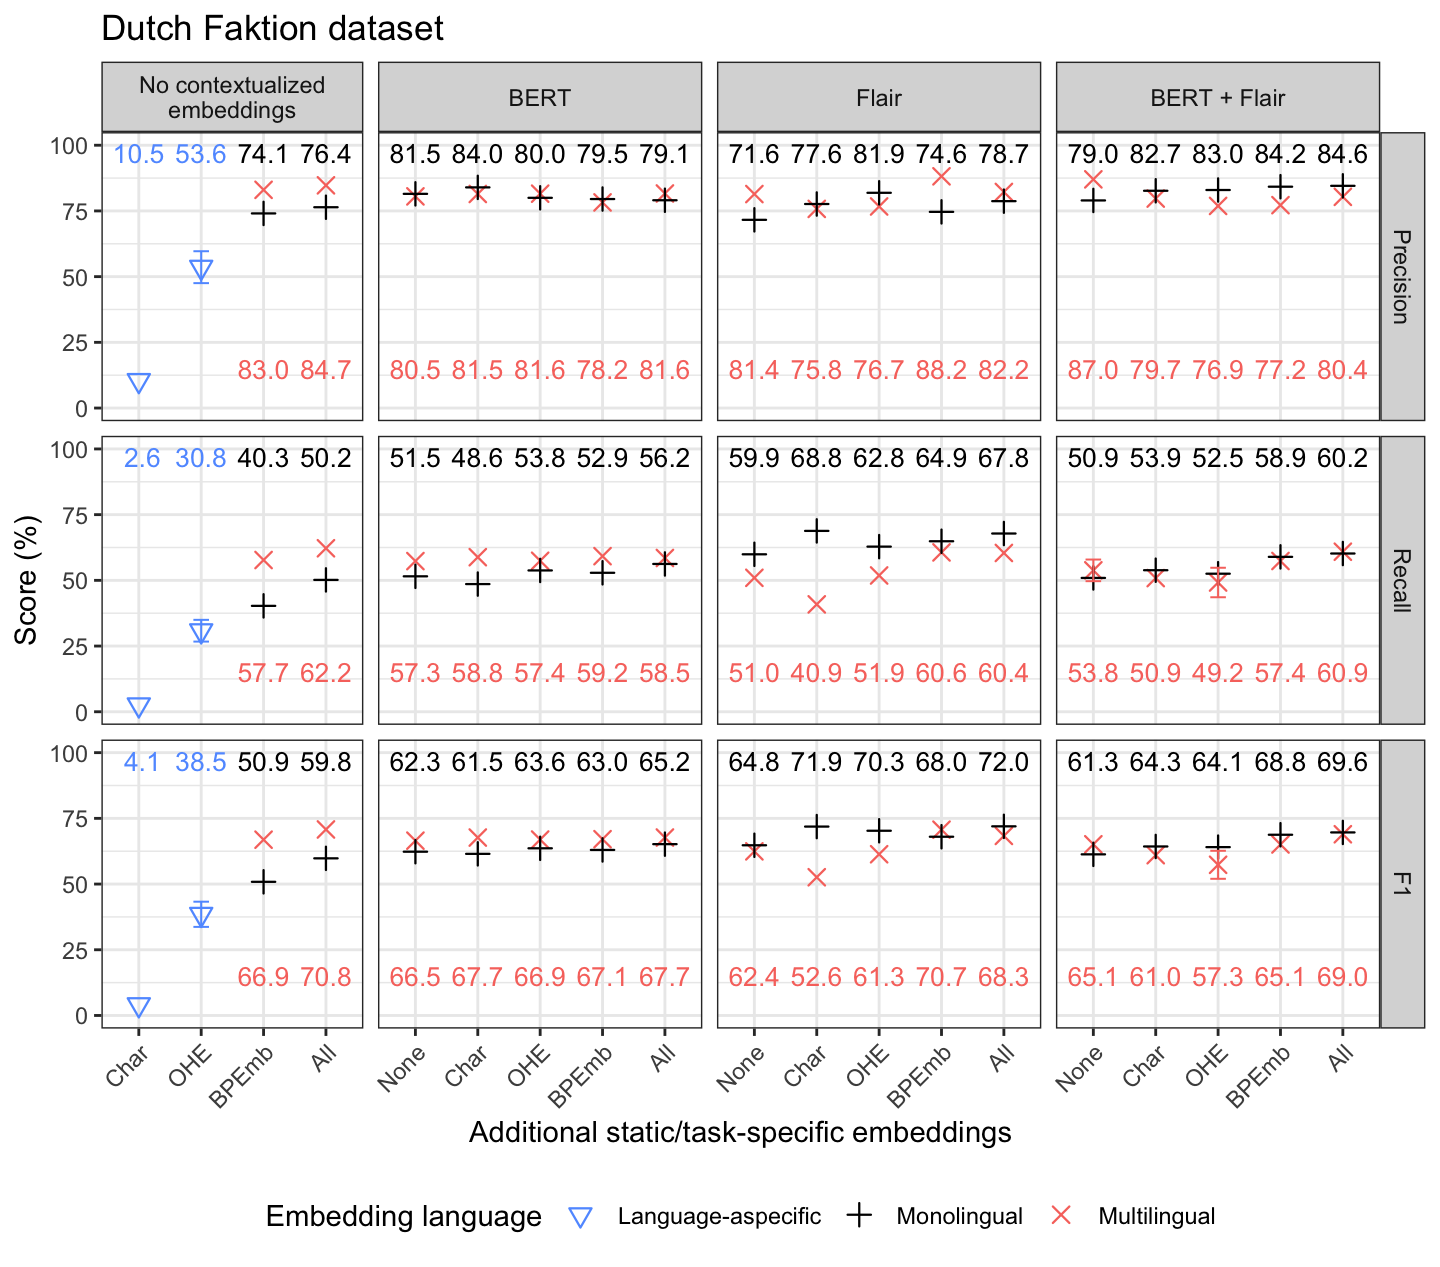
\includegraphics{Thesis_Arthur_Leloup_files/figure-latex/faktion-nl-fig-1} 

}

\caption{Test-set micro-average precision (top), recall (middle) and F1-scores (bottom) for the Dutch Faktion NER task. The results are grouped according to the constituents of each (stacked) embedding, consistent with Table \ref{tab:embeddings}. The contextualized embedding type, if present, is indicated on the different panels from left to right. The stacked/task-specific embedding type (if present) is shown on the x-axis. Symbols represent the mean score for \(k = 5\), error bars representing the standard error of the mean were shown where they exceeded the symbol size. The mean scores for every monolingual or multilingual model are indicated in the upper and lower region of each panel, respectively. \emph{BERT: BERTje (monolingual) or mBERT (multilingual); Flair: Flair Nl (monolingual) or mFlair (multilingual); Char: character embeddings; OHE: One Hot Embeddings; BPEmb: BytePair embeddings (Dutch/multilingual); All: concatenation of all static and task-specific embeddings, i.e. {[}Char + OHE + BPEmb + fastText{]} (for monolingual embeddings) or {[}Char + OHE + mBPEmb{]} (for multilingual embeddings).}}\label{fig:faktion-nl-fig}
\end{figure}



\begin{table}

\caption{\label{tab:faktion-nl-tab}Results acquired on the Dutch Faktion NER task with both monolingual and multilingual NER systems. Results are reported as mean ± standard error of the mean (k = 5). A complete overview of all results is provided in Table \ref{tab:apx-f-nl}.}
\centering
\begin{tabular}[t]{llll}
\toprule
Embedding type & Precision & Recall & F1-score\\
\midrule
\addlinespace[0.3em]
\multicolumn{4}{l}{\textbf{Monolingual embeddings}}\\
\hspace{1em}[all]: fastT + BPEmb + Char + OHE & 76.4 ± 7.5 & 50.2 ± 6.1 & 59.8 ± 5.4\\
\hspace{1em}BERTje & 81.5 ± 3.8 & 51.5 ± 4.8 & 62.3 ± 3.7\\
\hspace{1em}BERTje + [all] & 79.1 ± 2.9 & 56.2 ± 4.6 & 65.2 ± 3.1\\
\hspace{1em}Flair & 71.6 ± 5.2 & 59.9 ± 7.1 & 64.8 ± 6.1\\
\hspace{1em}Flair + [all] & 78.7 ± 7.3 & 67.8 ± 6.1 & \textbf{72.0 ± 4.8}\\
\hspace{1em}BERTje + Flair & 79.0 ± 4.0 & 50.9 ± 4.1 & 61.3 ± 2.9\\
\hspace{1em}BERTje + Flair + [all] & 84.6 ± 2.2 & 60.2 ± 5.4 & 69.6 ± 3.3\\
\addlinespace[0.3em]
\multicolumn{4}{l}{\textbf{Multilingual embeddings}}\\
\hspace{1em}[all]: mBPEmb + Char + OHE & 84.7 ± 5.0 & 62.2 ± 7.3 & \textbf{70.8 ± 4.8}\\
\hspace{1em}mBERT & 80.5 ± 5.0 & 57.3 ± 5.4 & 66.5 ± 5.1\\
\hspace{1em}mBERT + [all] & 81.6 ± 4.6 & 58.5 ± 5.7 & 67.7 ± 4.7\\
\hspace{1em}mFlair & 81.4 ± 5.3 & 51.0 ± 4.1 & 62.4 ± 4.3\\
\hspace{1em}mFlair + [all] & 82.2 ± 5.0 & 60.4 ± 7.8 & 68.3 ± 5.7\\
\hspace{1em}mBERT + mFlair & 87.0 ± 3.3 & 53.8 ± 9.2 & 65.1 ± 8.0\\
\hspace{1em}mBERT + mFlair + [all] & 80.4 ± 5.6 & 60.9 ± 6.5 & 69.0 ± 5.9\\
\bottomrule
\end{tabular}
\end{table}



The performance on the French Faktion dataset was, on average, lower in comparison with the Dutch dataset. However, it should be noted that the French dataset consisted of 2 entity categories while the Dutch dataset only contained a single entiy class to predict. The high-dimensional concatenations of CamemBERT together with all static and task-specific embeddings performed best, on average (F1-score: 54.6 ± 4.8 \%). In line with the previous observations, the differences between monolingual and multilingual embeddings were negligible (Table \ref{tab:faktion-fr-tab}), with the multilingual BytePair embeddings performing surprisingly well (Figure \ref{fig:faktion-multi-fig}). Among all multilingual embeddings that were tested for this dataset, estimated performance was, on average, highest for the concatenations of mFlair embeddings with mBytePair, OHE and character embeddings (F1-score: 54.5 ± 5.8 \%).

For the benchmark datasets, the performance as expressed in terms of the F1-score typically reflected a good balance between precision and recall. This was, however, not always the case for this dataset. Indeed, while the the French Flair-embeddings performed poorly in terms of the average F1-score (42.3 ± 3.8 \%), they did provide the highest precision, on average, among all monolingual systems (62.3 ± 6.6 \%). This is a direct result of the fact that the F1-score is defined as the harmonic mean of precision and recall, with the latter being low, on average, for this system (32.2 ± 2.8 \%), resulting in a low overall F1-score. For specific applications that require either a high precision or recall, it might make sense in these situations to not only consider their harmonic mean alone, but also evaluate the performance of the system in terms of precision and recall separately. An overview of all results is given in Table \ref{tab:apx-f-fr}.

\begin{figure}

{\centering 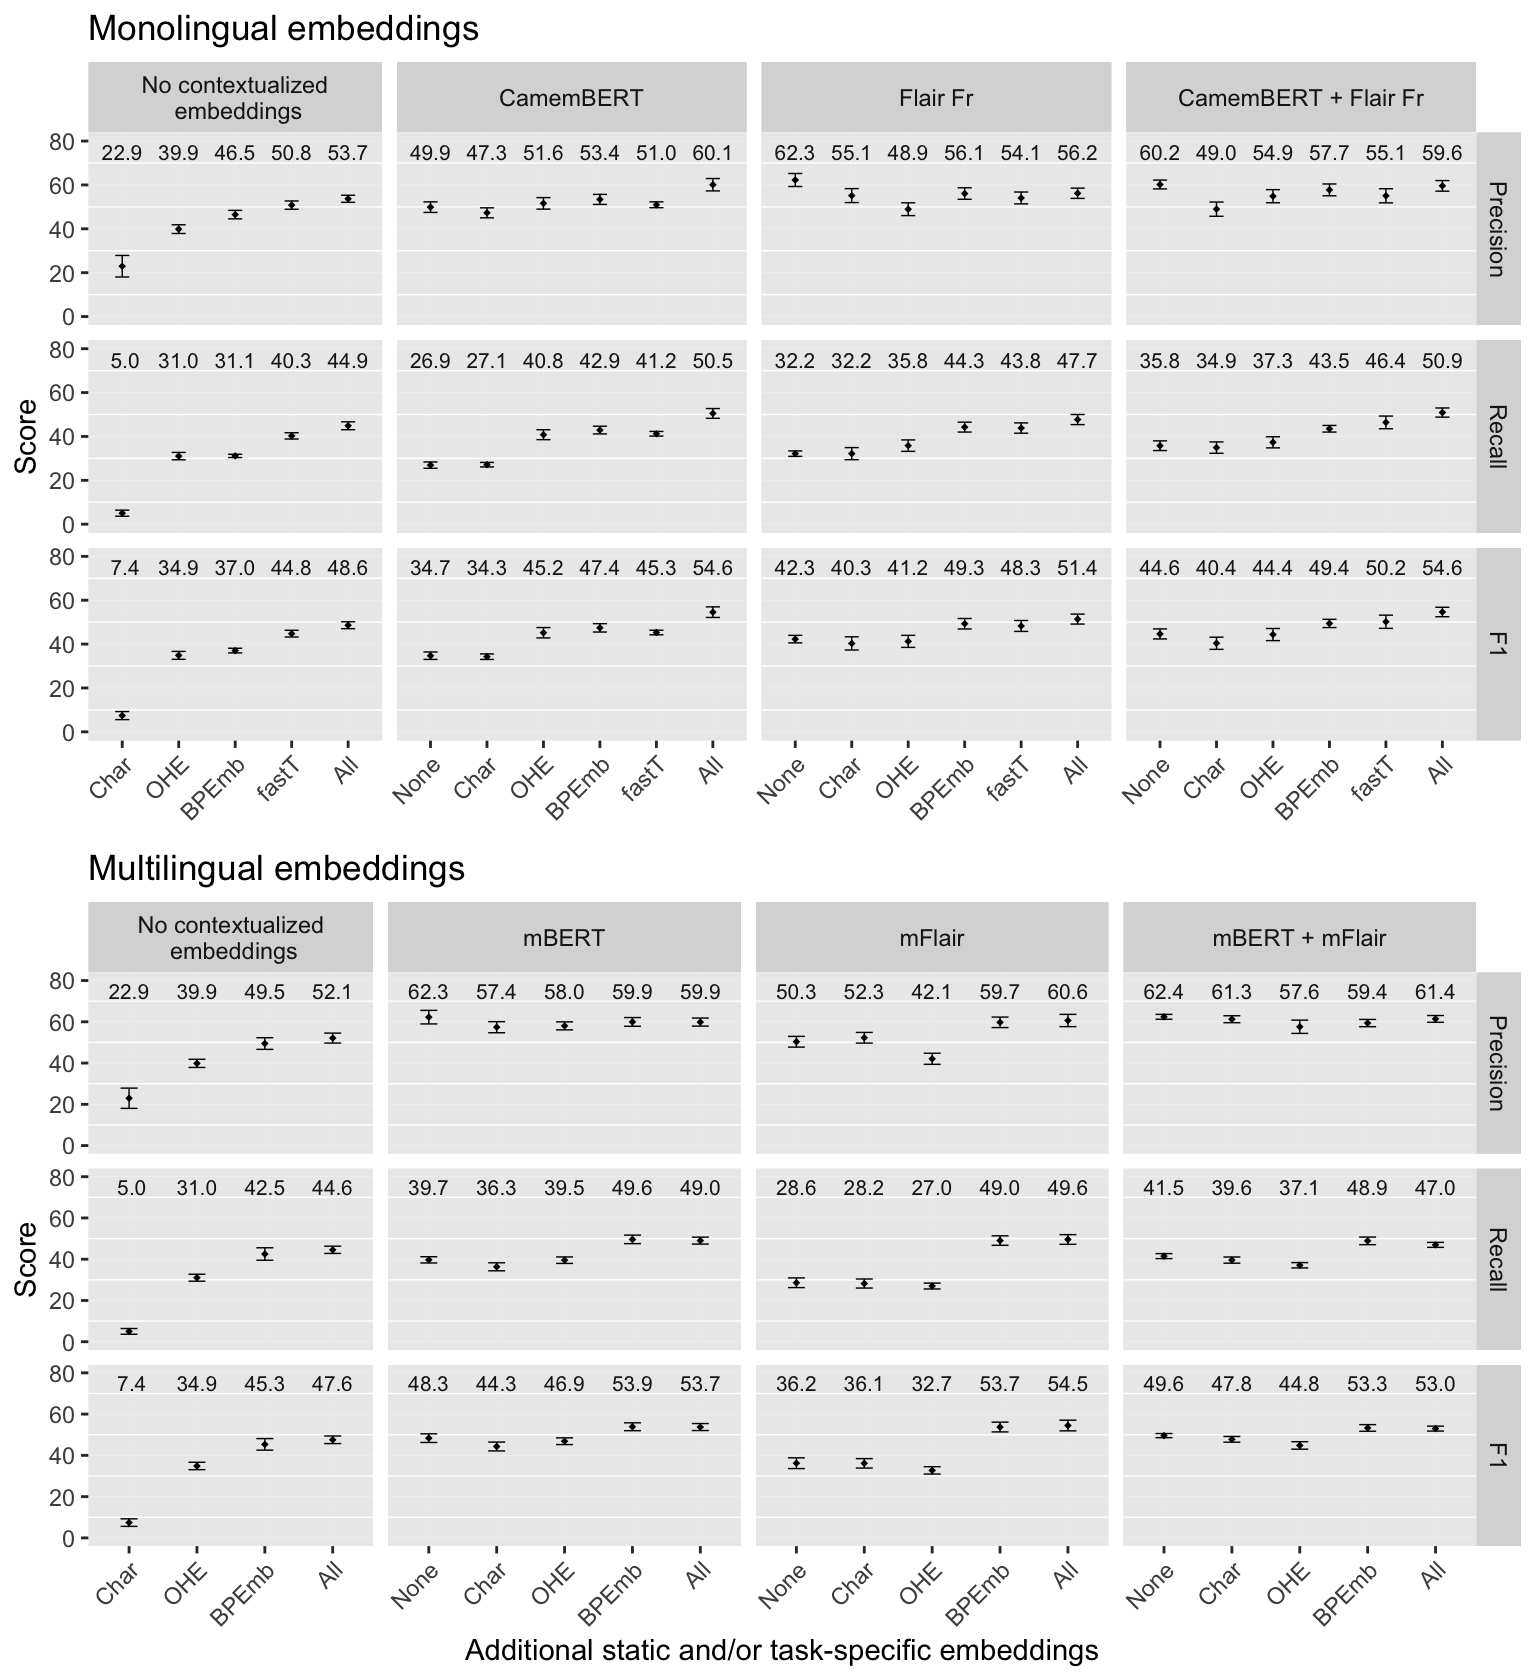
\includegraphics{Thesis_Arthur_Leloup_files/figure-latex/faktion-fr-fig-1} 

}

\caption{Test-set micro-average precision (top), recall (middle) and F1-scores (bottom) for the French Faktion NER task. The results are grouped according to the constituents of each (stacked) embedding, consistent with Table \ref{tab:embeddings}. The contextualized embedding type, if present, is indicated on the different panels from left to right. The stacked/task-specific embedding type (if present) is shown on the x-axis. Symbols represent the mean score for \(k = 5\), error bars representing the standard error of the mean were shown where they exceeded the symbol size. The mean scores for every monolingual or multilingual model are indicated in the upper and lower region of each panel, respectively. \emph{BERT: CamemBERT (monolingual) or mBERT (multilingual); Flair: Flair Fr (monolingual) or mFlair (multilingual); Char: character embeddings; OHE: One Hot Embeddings; BPEmb: BytePair embeddings (French/multilingual); All: concatenation of all static and task-specific embeddings, i.e. {[}Char + OHE + BPEmb + fastText{]} (for monolingual embeddings) or {[}Char + OHE + mBPEmb{]} (for multilingual embeddings).}}\label{fig:faktion-fr-fig}
\end{figure}



\begin{table}

\caption{\label{tab:faktion-fr-tab}Results acquired on the French Faktion NER task with both monolingual and multilingual NER systems. Results are reported as mean ± standard error of the mean (k = 5). A complete overview of all results is provided in Table \ref{tab:apx-f-nl}.}
\centering
\begin{tabular}[t]{llll}
\toprule
Embedding type & Precision & Recall & F1-score\\
\midrule
\addlinespace[0.3em]
\multicolumn{4}{l}{\textbf{Monolingual embeddings}}\\
\hspace{1em}[all]: fastT + BPEmb + Char + OHE & 53.7 ± 3.6 & 44.9 ± 4.0 & 48.6 ± 3.5\\
\hspace{1em}CamemBERT & 49.9 ± 5.4 & 26.9 ± 3.2 & 34.7 ± 3.8\\
\hspace{1em}CamemBERT + [all] & 60.1 ± 6.3 & 50.5 ± 5.0 & \textbf{54.6 ± 5.4}\\
\hspace{1em}Flair & 62.3 ± 6.6 & 32.2 ± 2.8 & 42.3 ± 3.8\\
\hspace{1em}Flair + [all] & 56.2 ± 5.2 & 47.7 ± 5.1 & 51.4 ± 5.1\\
\hspace{1em}CamemBERT + Flair & 60.2 ± 4.5 & 35.8 ± 4.9 & 44.6 ± 5.1\\
\hspace{1em}CamemBERT + Flair + [all] & 59.6 ± 5.4 & 50.9 ± 4.7 & 54.6 ± 4.8\\
\addlinespace[0.3em]
\multicolumn{4}{l}{\textbf{Multilingual embeddings}}\\
\hspace{1em}[all]: mBPEmb + Char + OHE & 52.1 ± 5.4 & 44.6 ± 3.9 & 47.6 ± 4.1\\
\hspace{1em}mBERT & 62.3 ± 7.3 & 39.7 ± 3.4 & 48.3 ± 4.7\\
\hspace{1em}mBERT + [all] & 59.9 ± 4.4 & 49.0 ± 3.8 & 53.7 ± 3.8\\
\hspace{1em}mFlair & 50.3 ± 5.8 & 28.6 ± 5.2 & 36.2 ± 5.8\\
\hspace{1em}mFlair + [all] & 60.6 ± 6.6 & 49.6 ± 5.3 & \textbf{54.5 ± 5.8}\\
\hspace{1em}mBERT + mFlair & 62.4 ± 2.6 & 41.5 ± 2.7 & 49.6 ± 2.2\\
\hspace{1em}mBERT + mFlair + [all] & 61.4 ± 3.7 & 47.0 ± 2.7 & 53.0 ± 2.7\\
\bottomrule
\end{tabular}
\end{table}



Lastly, a bilingual dataset was constructed by merging the Dutch and French Faktion datasets. Multilingual stacked embeddings (e.g.~mBERT, mBPEmb and character-feature embeddings) outperformed (either French or Dutch) monolingual embeddings (Figure \ref{fig:faktion-multi-fig}, Table \ref{tab:apx-f-bi}), with the the concatenation of mBERT, mBytePair and character embeddings performing best, on average (F1-score: 62.8 ± 1.9 \%, Table \ref{tab:apx-f-bi}). These results are in line with the results obtained on the multilingual benchmark dataset - at least with respect to the fact that multilingual clearly outperform monolingual embeddings in this setting, thus further supporting our research hypothesis. A complete overview of all results is provided in Table \ref{tab:apx-f-bi}.

\begin{table}

\caption{\label{tab:faktion-bi-tab}Results acquired on the multilingual (Dutch + French) Faktion NER task with both monolingual and multilingual NER systems. Results are reported as mean ± standard error of the mean (k = 5). A complete overview of all results is provided in Table \ref{tab:apx-f-nl}.}
\centering
\begin{tabular}[t]{llll}
\toprule
Embedding type & Precision & Recall & F1-score\\
\midrule
\addlinespace[0.3em]
\multicolumn{4}{l}{\textbf{Monolingual Dutch embeddings}}\\
\hspace{1em}[all]: fastT + BPEmb + Char + OHE & 67.3 ± 3.4 & 51.7 ± 4.3 & 58.3 ± 3.9\\
\hspace{1em}BERTje & 67.8 ± 3.6 & 32.5 ± 1.8 & 43.7 ± 1.6\\
\hspace{1em}BERTje + [all] & 65.9 ± 2.8 & 41.0 ± 3.3 & 50.2 ± 2.8\\
\hspace{1em}Flair & 67.1 ± 2.6 & 43.9 ± 3.6 & 52.7 ± 2.8\\
\hspace{1em}Flair + [all] & 69.8 ± 2.1 & 54.5 ± 1.6 & \textbf{61.1 ± 1.4}\\
\hspace{1em}BERTje + Flair & 67.1 ± 2.1 & 28.7 ± 1.8 & 40.1 ± 2.0\\
\hspace{1em}BERTje + Flair + [all] & 67.7 ± 2.6 & 39.5 ± 3.3 & 49.7 ± 3.0\\
\addlinespace[0.3em]
\multicolumn{4}{l}{\textbf{Monolingual French embeddings}}\\
\hspace{1em}[all]: fastT + BPEmb + Char + OHE & 66.0 ± 2.6 & 51.5 ± 3.4 & 57.7 ± 3.0\\
\hspace{1em}CamemBERT & 52.8 ± 5.2 & 22.2 ± 1.6 & 30.9 ± 1.8\\
\hspace{1em}CamemBERT + [all] & 67.4 ± 3.6 & 53.4 ± 3.0 & \textbf{59.5 ± 2.8}\\
\hspace{1em}Flair & 61.9 ± 4.1 & 28.0 ± 2.9 & 38.0 ± 2.8\\
\hspace{1em}Flair + [all] & 68.4 ± 3.9 & 49.9 ± 3.9 & 57.3 ± 3.3\\
\hspace{1em}CamemBERT + Flair & 72.0 ± 4.4 & 40.6 ± 3.8 & 51.6 ± 3.7\\
\hspace{1em}CamemBERT + Flair + [all] & 68.3 ± 1.8 & 51.8 ± 3.0 & 58.6 ± 1.6\\
\addlinespace[0.3em]
\multicolumn{4}{l}{\textbf{Multilingual embeddings}}\\
\hspace{1em}[all]: mBPEmb + Char + OHE & 73.7 ± 4.6 & 53.3 ± 3.4 & \textbf{61.6 ± 3.5}\\
\hspace{1em}mBERT & 68.1 ± 2.3 & 45.8 ± 2.6 & 54.6 ± 2.3\\
\hspace{1em}mBERT + [all] & 72.3 ± 3.2 & 52.3 ± 2.9 & 60.2 ± 2.0\\
\hspace{1em}mFlair & 68.2 ± 4.6 & 35.5 ± 3.1 & 46.3 ± 2.9\\
\hspace{1em}mFlair + [all] & 69.0 ± 2.9 & 50.8 ± 3.9 & 58.3 ± 3.3\\
\hspace{1em}mBERT + mFlair & 71.0 ± 2.6 & 41.8 ± 1.6 & 52.5 ± 1.5\\
\hspace{1em}mBERT + mFlair + [all] & 71.1 ± 3.3 & 51.2 ± 3.2 & 59.4 ± 3.0\\
\bottomrule
\end{tabular}
\end{table}



\begin{figure}

{\centering 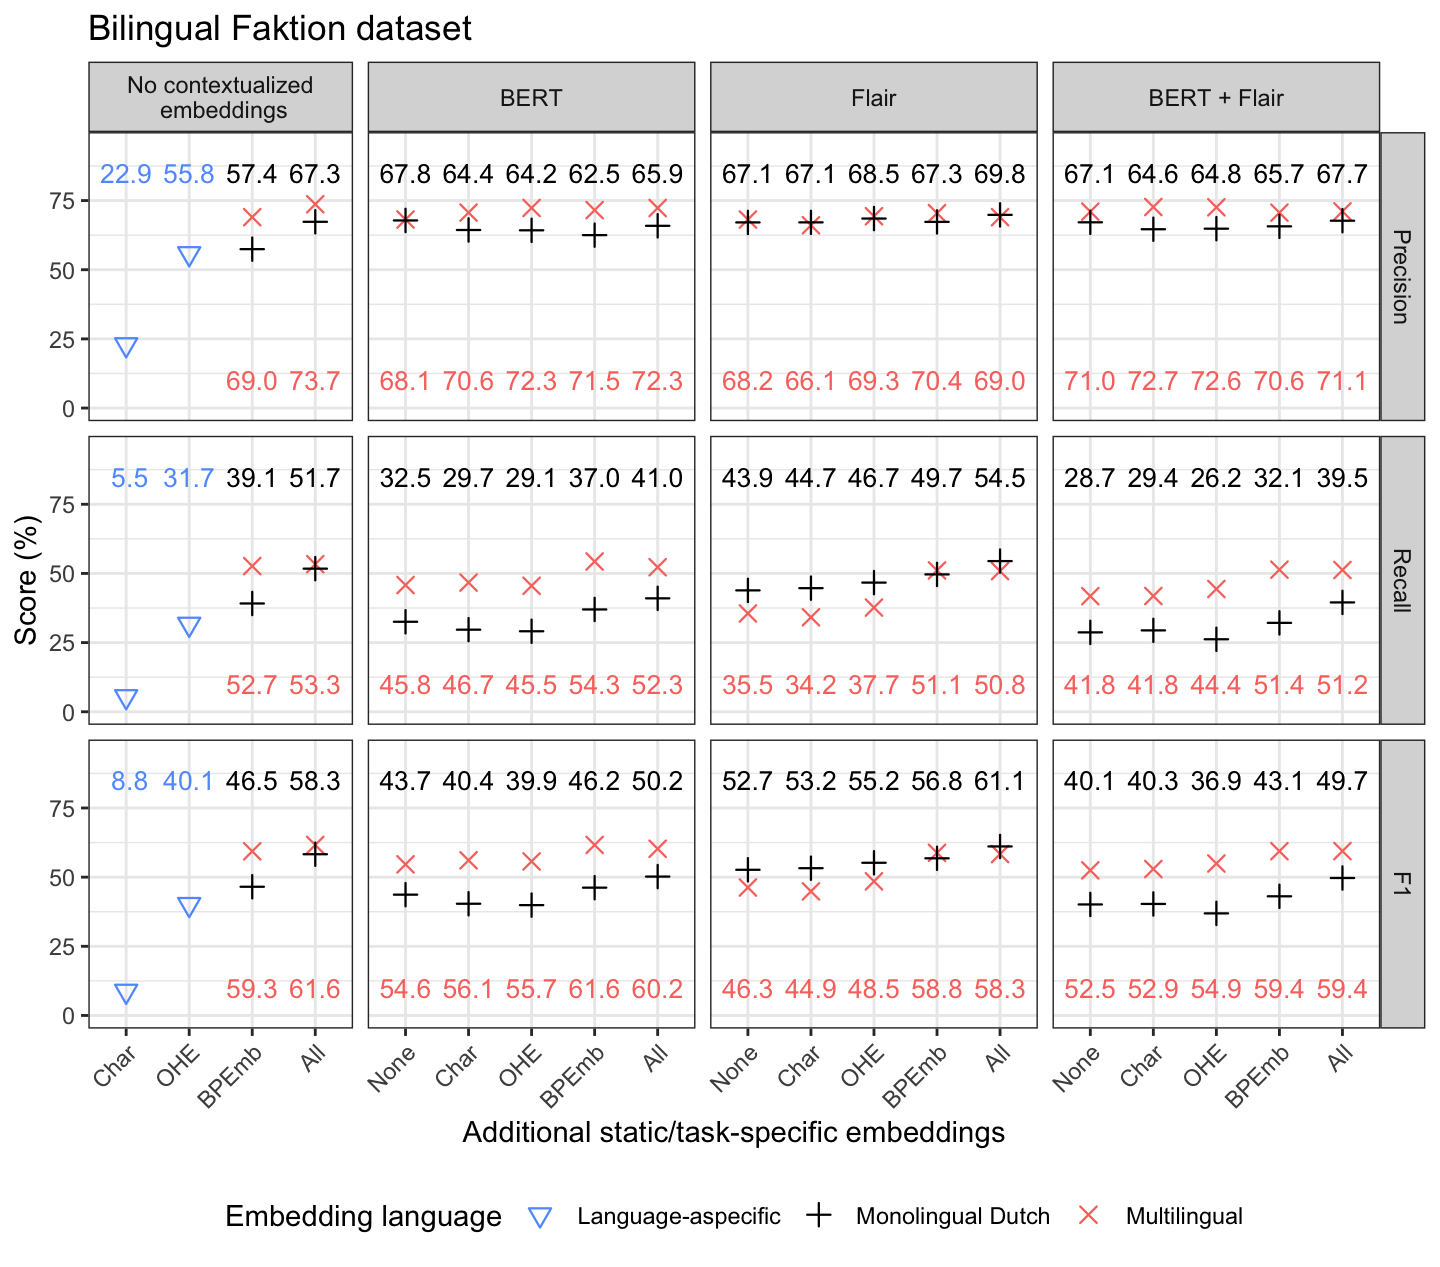
\includegraphics{Thesis_Arthur_Leloup_files/figure-latex/faktion-multi-fig-1} 

}

\caption{Test-set micro-average precision, recall and F1-scores for the multilingual (Dutch + French) Faktion NER task. The results are grouped according to the constituents of each (stacked) embedding, consistent with Table \ref{tab:embeddings}. The contextualized embedding type, if present, is indicated on the different panels from left to right. The stacked/task-specific embedding type (if present) is shown on the x-axis. Symbols represent the mean score for \(k = 5\), error bars representing the standard error of the mean were shown where they exceeded the symbol size. For clarity, the results for the French and English embeddings are omitted, a full overview of all results is provided in Table \ref{tab:apx-f-bi}. \emph{BERT: BERTje (monolingual) or mBERT (multilingual); Flair: Flair Nl (monolingual) or mFlair (multilingual); Char: character embeddings; OHE: One Hot Embeddings; BPEmb: BytePair embeddings (Dutch/multilingual); All: concatenation of all static and task-specific embeddings, i.e. {[}Char + OHE + BPEmb + fastText{]} (for monolingual embeddings) or {[}Char + OHE + mBPEmb{]} (for multilingual embeddings).}}\label{fig:faktion-multi-fig}
\end{figure}



\hypertarget{discussion}{%
\chapter{Discussion}\label{discussion}}

In this thesis, we aimed to evaluate how different monolingual and multilingual embeddings affected the performance of different monolingual and multilingual NER tasks. We addressed this question by performing a wide range of NER experiments on well-validated English, Dutch and French benchmark datasets, using different combinations of either monolingual or multilingual contextualized, static and/or task-specific word representations. Next, these systems were compared when the input data itself was multilingual. We were able to achieve F1-scores that were in accordance with state-of-the-art results reported in literature and confirmed earlier studies demonstrating that NER performance typically benefits from concatenating different embeddings together into single, high-dimensional representations. Monolingual embeddings outperformed multilingual embeddings on each of the monolingual NER tasks, but the differences were surprisingly small. Conversely, multilingual embeddings clearly outperformed monolingual embeddings on a multilingual NER task.

In addition, we evaluated how our monolingual and multilingual NER implementations performed on ``real-world'' datasets that were generated from OCR on scans of building plans in the context of a document annotation application developed by \href{https://www.faktion.com/}{Faktion}. Not surprisingly, the results on these small, noisy datasets were - on average - much lower as compared to the benchmark datasets. However, concatenating multiple embeddings together into single, high-dimensional representations again showed to be a successful approach to optimize NER performance. The fact that these datasets were not strictly monolingual was reflected in the performance differences between monolingual and multilingual embeddings: they performed similarly on the predominantly monolingual datasets, but multilingual embeddings outperformed monolingual embeddings when the input data was multilingual. These results suggest that state-of-the-art multilingual representations available today are ready to be implemented in practical applications like Metamaze, thus greatly reducing pipeline complexity at no cost of reduced performance.

\hypertarget{benchmarkt-datasets}{%
\section{Benchmarkt datasets}\label{benchmarkt-datasets}}

By using a state-of-the-art BiLSTM-CRF sequence labeling architecture \citep{akbik2018, huang2015, lample2016}, we were able to achieve results that were similar or slightly below results reported in literature for the CoNLL2003 task. While a direct comparison of our results with literature data was not the primary goal, it does indicate that our implementations provided a very useful framework to compare state-of-the-art monolingual and multilingual embeddings. The single point estimates of the extra-sample performances that were obtained for the different monolingual and multilingual embeddings did not allow us to thoroughly study the score distributions of all the implementations. We specifically opted to evaluate a wide range of different stacked combinations of monolingual and multilingual embeddings, in order to acquire a general overview on:

\begin{itemize}
\tightlist
\item
  Baseline performance with task-specific representations (i.e.~without transferring knowledge from static or contextualized representations)
\item
  The added value of static word or subword embeddings
\item
  The added value of state-of-the-art contextualized representations from pretrained Flair or BERT models
\end{itemize}

For most tasks, the Transformer-based BERT models (BERTje, CamemBERT, BERT and mBERT) outperformed the character-based Flair LMs, except for monolingual English, where the Flair model provided excellent representations that resulted in a similar performance on the NER task as compared to BERT-based representations. Interestingly, the difference between BERT-based and Flair-based embeddings was even more pronounced for multilingual models: mBERT clearly outperformed mFlair on all monolingual as well as multilingual benchmark datasets. In many cases, mFlair-based stacked embeddings were even outperformed by embeddings that did not include any contextualized representation obtained from a pretrained LM. There are several reasons that may account for this. Firstly, mBERT was trained on roughly 100 of the most common languages on Wikipedia, while \href{https://github.com/flairNLP/flair/issues/1099}{mFlair} was provided with the JW300 training corpus containing just over 2 billion tokens in more than 300 languages \citep{agic2019}. Given the significant cost involved into training a neural LM from scratch, the size of the training corpus is often limited. While corpus sizes in terms of number of tokens are not always directly comparable between models (e.g.~mBERT relied on subword tokenization and resampling strategies to account for the imbalance between different languages in the multilingual corpus), most models are pretrained on a corpora of at most a few billion tokens. This means that - in practice - the amount of training data for each specific language in a multilingual training corpus is inversely proportional to the number of different languages. Among many other differences between the mFlair and mBERT models, this might explain why mBERT seems to provide better representations for very common languages like English, Dutch or French. It might be interesting to evaluate this claim by comparing their performance in the context of NER in low-resource languages.

An interesting result was obtained with the Dutch version of BERT's Transformer architecture, BERTje \citep{devries2019}. Using the representations from its top layer, we achieved - to the best of our knowledge - a new state-of-the art on the Dutch CoNLL2002 task, outperforming the previous best result obtained with fine-tuning of mBERT \citep{wu2019} by 2.1 percentage points (from 90.9 \% to 93.0 \%). However, one should be cautious directly comparing these results. Firstly, computational resources did not allow us to perform multiple training runs for the different configurations. The stochastic nature of the training algorithm renders the BiLSTM-CRF architecture non-deterministic. Even though the obtained F1 point estimates are statistically unbiased, they are not necesarily representative for the entire score distribution. Indeed, empirical evidence has shown that the seed value chosen for the random number generator for state-of-the-art BiLSTM-CRF systems can result in F1-score differences as large as 1 percentage points on the CoNLL2003 task, which translates into a system being perceived as mediocre or state-of-the-art \citep{reimers2017}. In addition, our results on the CoNLL2002 dataset were obtained after (minor) preprocessing: 4/15806 sentences in the training set and 1/5195 sentences from the test set were removed for all experiments because they exceeded the maximum input sequence length for some models included in our evaluation. Nevertheless, all results for the different stackings based on BERTje embeddings (ranging from 91.5 \% (for BERTje embeddings alone) to 93.0 \% (for the largest stacked embedding)) consistently outperformed the result reported before \citep{devries2019, wu2019}. The importance of the sequence labeling architecture has been acknowledged already by the authors of the BERTje model \citep{devries2019} and our results seem to confirm that feeding the activations from BERTje's top layer into a BiLSTM-CRF model yields a considerable increase in performance as compared to fine-tuning BERTje or mBERT and using a regular softmax layer on top of the Transformer model to predict the NER labels.

Since we only used the activations for every first subtoken extracted from BERTje's top layer, we hypothesize that this result can be optimized even further. Indeed, earlier studies have indicated that performance of many NLP tasks can significanlty benefit from strategies that aim to specifically extract representations from the different layers of the pretrained Transformer LM. This includes manual per-layer analysis to find which layers encode information most relevant for the specific task or, alternative, learning a parametrized scalar mixture of the activations from the different layers to find the representation most relevant for the downstream task. Scalar mixing seems to outperform the best individual layer's representation on a wide range of NLP tasks \citep{liu2019} and was shown to be one of the main factors that determined the success of the representations obtained from the deep BiLSTM LM ELMo \citep{peters2018}.

The conclusions for the French WikiNER dataset were in accordance with the Dutch and English NER: monolingual systems outperformed multilingual ones, with a pronounced difference between Flair-based and Transformer-based representations. Given that this difference was not present in the results of the English CoNLL2003 task suggests that this is not merely a result of the intrinsic properties of the neural network architecture as such, but that - indeed - a character-based LM is able to provide excellent representations for downstream NER, if trained well. Given that the Dutch, French and multilingual Flair models have been trained by members of the Flair NLP community, while all other models (English Flair and the monolingual and multilingual versions of BERT) have been pretrained by research institutions might suggest that this difference can be - at least partly - attributed to the availability of resources to train these models. Even though the training of character-based LMs like Flair is order of magnitudes more efficient than traditional word-based BiLSTM LMs \citep{akbik2018}, it still requires the availability of enormous amounts of data and training for more than one week on a powerful GPU\footnote{\href{https://github.com/flairNLP/flair-lms}{GitHub: flairNLP/flair-lms}}.

Overall, our results for the benchmark datasets are in accordance with results reported in literature. Performance of the NER classifier consistently increased from representations learned from scratch directly onto the NER objective (OHE or character embeddings), to pretrained (static) vectors like fastText or BytePair embeddings, to contextualized representations obtained from large, pretrained neural LMs, as anticipated. Even though static word vectors provide only a single, ``average'' representation for polysemous words and are, hence, typically outperformed by contextualized representations on NER tasks, interestingly, performance seems to increase when static word vectors are concatenated to these contextualized representations, suggesting that they do add relevant information. This has been reported before, i.e.~Akbik and colleagues obtained state-of-the-art performance on the CoNLL2003 task using concatenated Flair, GloVe and character-level representations \citep{akbik2018}. An interesting study by Kawin Ethayarajh investigated how the different context-specific representations of the same word (obtained from e.g.~BERT) compared against static - non-contextualized - embeddings. They found that BERT's representations (especially the representations in the upper layers) were highly contextualized, in the sense that a single static embedding (the first principal component of the different context-dependent representations of a word) explained, on average, less than 5 \% of the total variance \citep{ethayarajh2019}. This might explain why concatenating the apparently highly context-dependent representation obtained from the last layer of BERT with a static word embedding that encodes more latent word-level semantics helps the NER classifier to perform well on the task.

Even though the large, high-dimensional stackings of different embedding types generally outperformed lower-dimensional representations obtained from a single pretrained model, the difference was typically small. However, the computational requirements to train models using these high-dimensional representations are much higher. In particular, the task-specific representations that are iteratively updated during training on the NER objective are essentially parameters of the BiLSTM-CRF model. As such, expanding the parameter space slows down the training procedure considerably and even though these high-dimensional representations seem to consistently (but slightly) outperform lower-dimensional embeddings, this balance between training efficiency and performance might be considered a limitation for some practical applications.

\hypertarget{faktion-datasets-2}{%
\section{Faktion datasets}\label{faktion-datasets-2}}

There were major differences between the characteristics of the Faktion datasets and the benchmark datasets discussed previously, which translated - not surprisingly - into different conclusions with respect to:

\begin{itemize}
\tightlist
\item
  The performance of monolingual and multilingual embeddings
\item
  The added value of obtaining contextualized representations from pretrained LMs
\end{itemize}

Firstly, the monolingal datasets were not strictly monolingual. This was reflected in the performance for monolingual and multilingual embeddings: while the former consistently outperformed the latter on the CoNLL and WikiNER datasets, there was virtually no difference for the Faktion datasets. In both the trilingual benchmark dataset as well as the bilingual Faktion dataset, the multilingual embeddings clearly outperformed any monolingual embedding. As mentioned previously, Metamaze's NER pipeline currently relies on the prediction of the dominant language in the input document to determine which (monolingual) NER system to use. Even though the advantage of monolingual embeddings over multilingual embeddings might be more pronounced when the documents are strictly monolingual, the results obtained here provide strong indications that for this type of input data, a multilingual NER pipeline might provide similar performance while completely omitting the need to maintain a separate language prediction step. In addition to this simplification, the fact that a multilingual system does not rely on an upstream language prediction step makes it more robust, as suggested by the presults obtained on the multilingual dataset.

Again - there was a clear trend of increasing NER performance when concatenating multiple embedding types into large, stacked embeddings. It was, however, surprising that the added value of contextualized embeddings from either pretrained Flair or BERT-like architectures was much less pronounced as compared to the benchmark NER tasks. Performance of the multilingual BytePair embeddings was, in general, surprisingly high, not only as compared directly to either French or Dutch monolingual BytePair embeddings, but especially when compared to the contextualized embeddings obtained from pretrained Flair or BERT. Condidering the nature of the Faktion datasets (i.e.~relatively noisy data obtained from OCR on scans of building plans) this might not come as a big surprise: many of the tokens contained punctuation or digits, were very short or even consisted of a single character. Since the ``linguistic knowledge'' acquired by these pretrained neural LMs are based on corpora that are chosen to be as representative as possible for ``general language'' (i.e.~news articles, Wikipedia, books, \ldots{}), they are expected to work best in this context. The fact that the semantic dependencies between tokens in these building plans are not necessarily representative for ``general language'', might partly explain why the acquired linguistic knowledge of pretrained BERT and Flair to provide contextualized token representations does not seem to help the NER classifier to perform well on this task. This has also been described in situations of e.g.~jargon-rich language like biomedical text. BioBERT - a BERT architecture pretrained on biomedical data - has been shown to outperform regular BERT for many NLP tasks specific to the field, including biomedical NER \citep{lee2020}. Unfortunately, training such a model entirely from scratch requires enormous amounts of data and comes at a significant cost. Since the weights of pretrained BERT have already very sensible values for many problems, a more efficient approach is to finetune the parameters of pretrained models using task-specific data. Indeed, this approach has shown to be very succesful for different scientific domains \citep{beltagy2019} or to enrich the language-specific vocabulary of multilingual models \citep{wang2019}.

As mentioned before, the Faktion datasets consisted of only one (for the Dutch dataset) or two (for the French and bilingual dataset) entity categories. For the latter, the vast majority of all entities (approximately 95 \%) belonged to a single category. In order to be consistent with the gold-standard evaluation procedure for NER tasks reported in literature, we reported micro-average entity-level precision, recall and F1-scores. Even though the F1-score is typically used to compare different NER systems and rank the performance on benchmark tasks like CoNLL, it should be mentioned that for some cases - including the highly imbalanced Faktion datasets - this does not provide a good representation of the per-class performance of the model. Since it is a weighted average of the F1-score per entity class, poor performance on the minority class is not well-reflected in the overall micro-average score. When optimizing NER classifiers for practical applications and depending on the relative cost of wrongly classifying entities belonging to the minority class, this should be taken into account. Also, as mentioned before, NER evaluation is typically performed on the entity-level, not on the token level. This means that optimizing an NER system for this metric essentially penalizes the model to be ``partially correct''. Indeed, a system that predicts ``In Prato {[}B-LOC{]} allo {[}I-LOC{]} Stelvio {[}I-LOC{]}'' as ``In Prato {[}B-LOC{]} allo Stelvio {[}B-LOC{]}'' makes 2 false positive predictions (Prato {[}B-LOC{]} and Stelvio {[}B-LOC{]}) and one false negative prediction (Prato {[}B-LOC{]} allo {[}I-LOC{]} Stelvio {[}I-LOC{]}). As a result, the system is penalized both in terms of precision (+ 2 FPs) and recall (+ 1 FN). In contrast, when the NER system predicts no entities at all, only a single false negative prediction is counted because the system failed to correctly predict the entity ``Prato {[}B-LOC{]} allo {[}I-LOC{]} Stelvio {[}I-LOC{]}'', thus only penalizing recall (+ 1 FN). This means that by optimizing a NER system on the entity-level F1-score, the system is essentially discouraged to predict these partial matches. One can argue that for many practical applications, the behavior of the first system is preferred, and optimizing for the F1-score might not be the best strategy in this case. This issue has been raised previously\footnote{\href{https://nlpers.blogspot.com/2006/08/doing-named-entity-recognition-dont.html}{``Doing Named Entity Recognition? Don't optimize for F1'' - Chris Manning (2006)}} and alternative evaluation strategies have been proposed to allow these partial matches to be taken into account \citep{chinchor1993, doddington2004, esuli2010}. However, these systems are typically quite complex and the vast majority of researchers adheres to the convention of evaluating NER systems according to micro-average F1-score. It might be interesting, however, to explore how other evaluation metrics compare to the way humans would naturally judge the performance of a NER system and how a lower F1-score might actually be preferable for practical applications like Metamaze.

\hypertarget{conclusion}{%
\section{Conclusion}\label{conclusion}}

To conclude, we discuss some limitations of the work presented here as well as some future perspectives. The main goal of this thesis was to acquire an overview on how different monolingual and multilingual embeddings affect NER performance in different situations. With this goal in mind, we aimed to keep the model parameters and embedding types consistent between experiments. While this provided a good overview on the relative contribution of the different embedding types to NER performance in many different situations, we did not specifically aim to maximize performance of each individual system or provide a robust analysis on the score distributions of each system. However, given the stochastic nature of the training algorithms, one should consider the entire score distribution in order to formally infer whether different monolingual and multilingual systems perform - on average - differently. It might be interesting to perform such a study in the future. In addition, when it comes to implementing a system for a practical application, it is very likely that performance will benefit from optimization. In particular, we did not explore which layers of the Transformer models provided the most informative representations for the NER task but focused predominantly on the comparison between monolingual and multilingual systems based on the activations from the top layer only. It might be interesting to explore to what extend optimization strategies can improve both monolingual as well as multilingual NER performance further. These optimization steps might be equally effective in improving the results on the Faktion datasets, even though - in general - the advantage of these state-of-the-art contextualized embeddings from pretrained neural LMs was more limited. It might be very interesting to explore how fine-tuning the weights of mBERT with data more relevant to this specific problem might result in representations that are able to improve the performance of the NER system in this specific context even further. Nevertheless, even without extensive optimization, our results indicate that the multilingual embeddings that were evaluated during this thesis have the ability to significantly reduce the complexity of the current document annotation pipeline of Metamaze, by omitting the need for a separate language-prediction step, while achieving excellent performance compared to monolingual systems, in particular when the language heterogeneity of the dataset grows.

\newpage

\hypertarget{appendix-appendix}{%
\appendix}


\hypertarget{benchmark-results}{%
\chapter{Benchmark results}\label{benchmark-results}}

In this appendix, we provide an overview of the entity-level test-set precision, recall and F1-scores for all NER experiments on the English CoNLL2003 dataset (Table \ref{tab:apx-en}), the Dutch CoNLL2002 dataset (Table \ref{tab:apx-nl}), the French WikiNER dataset (Table \ref{tab:apx-fr}) and the multilingual benchmark dataset (Table \ref{tab:apx-trired}), as described in chapter \ref{methods}. Large stackings of static and task-specific embeddings are referred to as `All', indicating - for monolingual embeddings - the concatenation of character (Char) embeddings, one hot word type embeddings (OHE), BytePair embeddings (BPEmb) and fastText (fastT) embeddings for the respective languages. For multilingual embeddings, ``All'' refers to the concatenation of multilingual BytePair embeddings (mBPEmb), together with OHE and character embeddings. Details are given in the text.

\begingroup\fontsize{10}{12}\selectfont

\begin{longtable}[t]{llrrr}
\caption{\label{tab:apx-en}Overview of all results for the English CoNLL2003 task. The reported scores are the result of a single training run.}\\
\toprule
Contextualized embedding & Static/task-spec. embedding & Precision & Recall & F1-score\\
\midrule
\endfirsthead
\caption[]{\label{tab:apx-en}Overview of all results for the English CoNLL2003 task. The reported scores are the result of a single training run. \textit{(continued)}}\\
\toprule
Contextualized embedding & Static/task-spec. embedding & Precision & Recall & F1-score\\
\midrule
\endhead
\
\endfoot
\bottomrule
\endlastfoot
\addlinespace[0.3em]
\multicolumn{5}{l}{\textbf{Only task-specific embeddings}}\\
\hspace{1em}None & Char & 74.1 & 73.9 & 74.0\\
\hspace{1em}None & OHE & 80.7 & 70.8 & 75.4\\
\addlinespace[0.3em]
\multicolumn{5}{l}{\textbf{Monolingual embeddings}}\\
\hspace{1em}None & BPEmb & 86.7 & 84.9 & 85.7\\
\hspace{1em}None & fastT & 90.4 & 89.9 & 90.1\\
\hspace{1em}None & All & 90.8 & 90.9 & 90.9\\
\hspace{1em}BERT & None & 91.3 & 91.1 & 91.2\\
\hspace{1em}BERT & Char & 91.1 & 91.2 & 91.2\\
\hspace{1em}BERT & OHE & 91.1 & 90.5 & 90.8\\
\hspace{1em}BERT & BPEmb & 91.1 & 91.5 & 91.3\\
\hspace{1em}BERT & fastT & 91.7 & 92.0 & 91.8\\
\hspace{1em}BERT & All & 91.9 & 92.3 & 92.1\\
\hspace{1em}Flair & None & 90.3 & 90.8 & 90.5\\
\hspace{1em}Flair & Char & 90.6 & 91.1 & 90.8\\
\hspace{1em}Flair & OHE & 90.1 & 90.8 & 90.4\\
\hspace{1em}Flair & BPEmb & 91.7 & 92.2 & 91.9\\
\hspace{1em}Flair & fastT & 92.0 & 92.6 & 92.3\\
\hspace{1em}Flair & All & 92.3 & 92.4 & 92.3\\
\hspace{1em}BERT + Flair & None & 91.3 & 91.9 & 91.6\\
\hspace{1em}BERT + Flair & Char & 91.3 & 92.1 & 91.7\\
\hspace{1em}BERT + Flair & OHE & 91.6 & 92.0 & 91.8\\
\hspace{1em}BERT + Flair & BPEmb & 91.8 & 92.2 & 92.0\\
\hspace{1em}BERT + Flair & fastT & 91.7 & 92.3 & 92.0\\
\hspace{1em}BERT + Flair & All & 92.3 & 92.7 & 92.5\\
\addlinespace[0.3em]
\multicolumn{5}{l}{\textbf{Multilingual embeddings}}\\
\hspace{1em}None & BPEmb & 86.0 & 83.2 & 84.5\\
\hspace{1em}None & All & 88.3 & 87.8 & 88.0\\
\hspace{1em}mBERT & None & 90.8 & 90.6 & 90.7\\
\hspace{1em}mBERT & Char & 90.6 & 91.4 & 91.0\\
\hspace{1em}mBERT & OHE & 90.5 & 90.9 & 90.6\\
\hspace{1em}mBERT & BPEmb & 91.0 & 91.7 & 91.3\\
\hspace{1em}mBERT & All & 91.0 & 91.9 & 91.4\\
\hspace{1em}mFlair & None & 84.6 & 84.8 & 84.7\\
\hspace{1em}mFlair & Char & 84.6 & 85.0 & 84.8\\
\hspace{1em}mFlair & OHE & 85.8 & 85.9 & 85.8\\
\hspace{1em}mFlair & BPEmb & 87.6 & 88.4 & 88.0\\
\hspace{1em}mFlair & All & 87.6 & 88.2 & 87.9\\
\hspace{1em}mBERT + mFlair & None & 90.5 & 91.2 & 90.9\\
\hspace{1em}mBERT + mFlair & Char & 90.5 & 91.2 & 90.9\\
\hspace{1em}mBERT + mFlair & OHE & 90.8 & 91.4 & 91.1\\
\hspace{1em}mBERT + mFlair & BPEmb & 91.0 & 92.0 & 91.5\\
\hspace{1em}mBERT + mFlair & All & 90.8 & 91.4 & 91.1\\*
\end{longtable}
\endgroup{}

\newpage

\begingroup\fontsize{10}{12}\selectfont

\begin{longtable}[t]{llrrr}
\caption{\label{tab:apx-nl}Overview of all results for the Dutch CoNLL2002 task. The reported scores are the result of a single training run.}\\
\toprule
Contextualized embedding & Static/task-spec. embedding & Precision & Recall & F1-score\\
\midrule
\endfirsthead
\caption[]{\label{tab:apx-nl}Overview of all results for the Dutch CoNLL2002 task. The reported scores are the result of a single training run. \textit{(continued)}}\\
\toprule
Contextualized embedding & Static/task-spec. embedding & Precision & Recall & F1-score\\
\midrule
\endhead
\
\endfoot
\bottomrule
\endlastfoot
\addlinespace[0.3em]
\multicolumn{5}{l}{\textbf{Only task-specific embeddings}}\\
\hspace{1em}None & Char & 68.9 & 67.2 & 67.8\\
\hspace{1em}None & OHE & 80.3 & 50.9 & 61.7\\
\addlinespace[0.3em]
\multicolumn{5}{l}{\textbf{Monolingual embeddings}}\\
\hspace{1em}None & BPEmb & 83.1 & 74.6 & 78.0\\
\hspace{1em}None & fastT & 86.7 & 75.1 & 79.7\\
\hspace{1em}None & All & 88.1 & 86.8 & 87.4\\
\hspace{1em}BERTje & None & 91.8 & 91.3 & 91.5\\
\hspace{1em}BERTje & Char & 92.6 & 91.9 & 92.2\\
\hspace{1em}BERTje & OHE & 92.2 & 91.4 & 91.8\\
\hspace{1em}BERTje & BPEmb & 92.5 & 91.6 & 92.0\\
\hspace{1em}BERTje & fastT & 92.7 & 91.8 & 92.2\\
\hspace{1em}BERTje & All & 93.1 & 92.2 & 92.6\\
\hspace{1em}Flair Nl & None & 86.9 & 86.2 & 86.4\\
\hspace{1em}Flair Nl & Char & 86.8 & 86.3 & 86.4\\
\hspace{1em}Flair Nl & OHE & 87.4 & 86.2 & 86.8\\
\hspace{1em}Flair Nl & BPEmb & 88.7 & 88.3 & 88.4\\
\hspace{1em}Flair Nl & fastT & 89.8 & 89.2 & 89.4\\
\hspace{1em}Flair Nl & All & 90.2 & 89.3 & 89.7\\
\hspace{1em}BERTje + Flair Nl & None & 92.4 & 92.5 & 92.4\\
\hspace{1em}BERTje + Flair Nl & Char & 92.8 & 92.8 & 92.8\\
\hspace{1em}BERTje + Flair Nl & OHE & 92.6 & 92.3 & 92.4\\
\hspace{1em}BERTje + Flair Nl & BPEmb & 92.9 & 92.7 & 92.8\\
\hspace{1em}BERTje + Flair Nl & fastT & 93.1 & 92.8 & 92.9\\
\hspace{1em}BERTje + Flair Nl & All & 93.1 & 93.0 & 93.0\\
\addlinespace[0.3em]
\multicolumn{5}{l}{\textbf{Multilingual embeddings}}\\
\hspace{1em}None & BPEmb & 85.6 & 67.5 & 75.1\\
\hspace{1em}None & All & 82.8 & 80.0 & 81.3\\
\hspace{1em}mBERT & None & 89.2 & 88.5 & 88.8\\
\hspace{1em}mBERT & Char & 89.6 & 88.5 & 89.0\\
\hspace{1em}mBERT & OHE & 89.9 & 89.1 & 89.5\\
\hspace{1em}mBERT & BPEmb & 89.9 & 89.3 & 89.5\\
\hspace{1em}mBERT & All & 90.6 & 89.4 & 90.0\\
\hspace{1em}mFlair & None & 79.8 & 78.8 & 79.1\\
\hspace{1em}mFlair & Char & 79.4 & 78.7 & 78.9\\
\hspace{1em}mFlair & OHE & 80.7 & 78.7 & 79.6\\
\hspace{1em}mFlair & BPEmb & 83.8 & 82.8 & 83.2\\
\hspace{1em}mFlair & All & 84.7 & 82.6 & 83.6\\
\hspace{1em}mBERT + mFlair & None & 89.8 & 89.4 & 89.5\\
\hspace{1em}mBERT + mFlair & Char & 89.9 & 89.3 & 89.5\\
\hspace{1em}mBERT + mFlair & OHE & 90.3 & 89.1 & 89.6\\
\hspace{1em}mBERT + mFlair & BPEmb & 90.5 & 89.9 & 90.1\\
\hspace{1em}mBERT + mFlair & All & 90.4 & 89.8 & 90.1\\*
\end{longtable}
\endgroup{}

\newpage

\begingroup\fontsize{10}{12}\selectfont

\begin{longtable}[t]{llrrr}
\caption{\label{tab:apx-fr}Overview of all results for the French WikiNER task. The reported scores are the result of a single training run.}\\
\toprule
Contextualized embedding & Static/task-spec. embedding & Precision & Recall & F1-score\\
\midrule
\endfirsthead
\caption[]{\label{tab:apx-fr}Overview of all results for the French WikiNER task. The reported scores are the result of a single training run. \textit{(continued)}}\\
\toprule
Contextualized embedding & Static/task-spec. embedding & Precision & Recall & F1-score\\
\midrule
\endhead
\
\endfoot
\bottomrule
\endlastfoot
\addlinespace[0.3em]
\multicolumn{5}{l}{\textbf{Only task-specific embeddings}}\\
\hspace{1em}None & Char & 61.0 & 60.5 & 60.2\\
\hspace{1em}None & OHE & 70.5 & 65.2 & 67.4\\
\addlinespace[0.3em]
\multicolumn{5}{l}{\textbf{Monolingual embeddings}}\\
\hspace{1em}None & BPEmb & 77.3 & 75.5 & 76.1\\
\hspace{1em}None & fastT & 79.3 & 74.7 & 76.6\\
\hspace{1em}None & All & 84.0 & 83.9 & 83.9\\
\hspace{1em}CamemBERT & None & 84.5 & 84.8 & 84.6\\
\hspace{1em}CamemBERT & Char & 86.0 & 86.0 & 86.0\\
\hspace{1em}CamemBERT & OHE & 86.4 & 86.4 & 86.3\\
\hspace{1em}CamemBERT & BPEmb & 85.4 & 85.5 & 85.4\\
\hspace{1em}CamemBERT & fastT & 86.7 & 86.6 & 86.6\\
\hspace{1em}CamemBERT & All & 86.3 & 86.4 & 86.3\\
\hspace{1em}Flair Fr & None & 79.1 & 80.0 & 79.4\\
\hspace{1em}Flair Fr & Char & 80.8 & 81.6 & 81.0\\
\hspace{1em}Flair Fr & OHE & 82.3 & 82.7 & 82.5\\
\hspace{1em}Flair Fr & BPEmb & 83.2 & 83.5 & 83.2\\
\hspace{1em}Flair Fr & fastT & 84.6 & 84.8 & 84.6\\
\hspace{1em}Flair Fr & All & 85.2 & 85.3 & 85.2\\
\hspace{1em}CamemBERT + Flair Fr & None & 86.2 & 86.2 & 86.1\\
\hspace{1em}CamemBERT + Flair Fr & Char & 86.7 & 86.7 & 86.7\\
\hspace{1em}CamemBERT + Flair Fr & OHE & 86.2 & 86.0 & 86.1\\
\hspace{1em}CamemBERT + Flair Fr & BPEmb & 87.1 & 86.8 & 86.9\\
\hspace{1em}CamemBERT + Flair Fr & fastT & 87.6 & 87.5 & 87.6\\
\hspace{1em}CamemBERT + Flair Fr & All & 87.4 & 87.4 & 87.4\\
\addlinespace[0.3em]
\multicolumn{5}{l}{\textbf{Multilingual embeddings}}\\
\hspace{1em}None & BPEmb & 77.6 & 74.1 & 75.6\\
\hspace{1em}None & All & 80.2 & 80.8 & 80.4\\
\hspace{1em}mBERT & None & 85.5 & 85.4 & 85.4\\
\hspace{1em}mBERT & Char & 84.8 & 84.8 & 84.8\\
\hspace{1em}mBERT & OHE & 85.3 & 85.3 & 85.2\\
\hspace{1em}mBERT & BPEmb & 86.4 & 86.6 & 86.5\\
\hspace{1em}mBERT & All & 85.3 & 85.0 & 85.1\\
\hspace{1em}mFlair & None & 74.4 & 75.7 & 74.7\\
\hspace{1em}mFlair & Char & 76.8 & 77.8 & 77.1\\
\hspace{1em}mFlair & OHE & 79.5 & 80.1 & 79.8\\
\hspace{1em}mFlair & BPEmb & 81.2 & 81.9 & 81.5\\
\hspace{1em}mFlair & All & 81.0 & 81.6 & 81.2\\
\hspace{1em}mBERT + mFlair & None & 84.8 & 84.9 & 84.8\\
\hspace{1em}mBERT + mFlair & Char & 85.3 & 85.5 & 85.4\\
\hspace{1em}mBERT + mFlair & OHE & 85.0 & 85.0 & 85.0\\
\hspace{1em}mBERT + mFlair & BPEmb & 85.6 & 85.7 & 85.6\\
\hspace{1em}mBERT + mFlair & All & 86.2 & 86.3 & 86.2\\*
\end{longtable}
\endgroup{}

\newpage

\begingroup\fontsize{10}{12}\selectfont

\begin{longtable}[t]{llrrr}
\caption{\label{tab:apx-trired}Overview of all results for the multilingual (En + Nl + Fr) NER task. The reported scores are the result of a single training run.}\\
\toprule
Contextualized embedding & Static/task-spec. embedding & Precision & Recall & F1-score\\
\midrule
\endfirsthead
\caption[]{\label{tab:apx-trired}Overview of all results for the multilingual (En + Nl + Fr) NER task. The reported scores are the result of a single training run. \textit{(continued)}}\\
\toprule
Contextualized embedding & Static/task-spec. embedding & Precision & Recall & F1-score\\
\midrule
\endhead
\
\endfoot
\bottomrule
\endlastfoot
\addlinespace[0.3em]
\multicolumn{5}{l}{\textbf{Only task-specific embeddings}}\\
\hspace{1em}None & Char & 61.6 & 60.0 & 60.4\\
\hspace{1em}None & OHE & 68.3 & 55.2 & 60.8\\
\addlinespace[0.3em]
\multicolumn{5}{l}{\textbf{English embeddings}}\\
\hspace{1em}None & BPEmb & 79.7 & 65.8 & 71.5\\
\hspace{1em}None & fastT & 80.8 & 73.2 & 76.3\\
\hspace{1em}None & All & 84.4 & 83.8 & 84.0\\
\hspace{1em}BERT & None & 82.0 & 81.0 & 81.4\\
\hspace{1em}BERT & Char & 82.8 & 82.1 & 82.4\\
\hspace{1em}BERT & OHE & 82.2 & 81.0 & 81.5\\
\hspace{1em}BERT & BPEmb & 83.5 & 82.5 & 83.0\\
\hspace{1em}BERT & fastT & 84.3 & 83.3 & 83.8\\
\hspace{1em}BERT & All & 85.0 & 84.2 & 84.6\\
\hspace{1em}Flair & None & 79.5 & 79.2 & 79.2\\
\hspace{1em}Flair & Char & 80.2 & 80.1 & 80.1\\
\hspace{1em}Flair & OHE & 80.8 & 80.8 & 80.7\\
\hspace{1em}Flair & BPEmb & 83.3 & 83.0 & 83.1\\
\hspace{1em}Flair & All & 85.2 & 85.1 & 85.1\\
\hspace{1em}BERT + Flair & None & 83.5 & 83.4 & 83.4\\
\hspace{1em}BERT + Flair & Char & 84.2 & 83.6 & 83.8\\
\hspace{1em}BERT + Flair & OHE & 83.7 & 82.8 & 83.2\\
\hspace{1em}BERT + Flair & BPEmb & 84.2 & 83.7 & 83.9\\
\hspace{1em}BERT + Flair & All & 85.3 & 85.1 & 85.2\\
\addlinespace[0.3em]
\multicolumn{5}{l}{\textbf{Dutch embeddings}}\\
\hspace{1em}None & BPEmb & 78.7 & 67.2 & 71.9\\
\hspace{1em}None & fastT & 83.1 & 72.8 & 77.1\\
\hspace{1em}None & All & 83.5 & 82.9 & 83.1\\
\hspace{1em}BERTje & None & 80.1 & 77.4 & 78.6\\
\hspace{1em}BERTje & Char & 80.2 & 79.2 & 79.7\\
\hspace{1em}BERTje & OHE & 80.6 & 77.5 & 79.0\\
\hspace{1em}BERTje & BPEmb & 82.9 & 81.7 & 82.3\\
\hspace{1em}BERTje & fastT & 84.3 & 83.5 & 83.9\\
\hspace{1em}BERTje & All & 85.0 & 84.8 & 84.9\\
\hspace{1em}Flair Nl & None & 79.1 & 79.7 & 79.3\\
\hspace{1em}Flair Nl & Char & 79.4 & 79.9 & 79.5\\
\hspace{1em}Flair Nl & OHE & 80.3 & 80.7 & 80.4\\
\hspace{1em}Flair Nl & BPEmb & 81.6 & 82.3 & 81.9\\
\hspace{1em}Flair Nl & fastT & 84.0 & 84.2 & 84.0\\
\hspace{1em}Flair Nl & All & 84.1 & 84.2 & 84.1\\
\hspace{1em}BERTje + Flair Nl & None & 80.7 & 80.6 & 80.6\\
\hspace{1em}BERTje + Flair Nl & Char & 80.5 & 80.6 & 80.5\\
\hspace{1em}BERTje + Flair Nl & OHE & 81.5 & 81.1 & 81.2\\
\hspace{1em}BERTje + Flair Nl & BPEmb & 83.0 & 83.4 & 83.1\\
\hspace{1em}BERTje + Flair Nl & fastT & 83.7 & 83.9 & 83.7\\
\hspace{1em}BERTje + Flair Nl & All & 85.2 & 85.8 & 85.5\\
\addlinespace[0.3em]
\multicolumn{5}{l}{\textbf{French embeddings}}\\
\hspace{1em}None & BPEmb & 77.9 & 64.6 & 69.9\\
\hspace{1em}None & fastT & 82.5 & 71.8 & 76.2\\
\hspace{1em}None & All & 83.8 & 83.0 & 83.3\\
\hspace{1em}CamemBERT & None & 81.0 & 79.6 & 80.2\\
\hspace{1em}CamemBERT & Char & 80.8 & 80.2 & 80.5\\
\hspace{1em}CamemBERT & OHE & 82.1 & 80.5 & 81.2\\
\hspace{1em}CamemBERT & BPEmb & 83.1 & 82.4 & 82.7\\
\hspace{1em}CamemBERT & fastT & 85.5 & 85.1 & 85.3\\
\hspace{1em}CamemBERT & All & 86.1 & 85.6 & 85.8\\
\hspace{1em}Flair Fr & None & 76.5 & 75.8 & 76.1\\
\hspace{1em}Flair Fr & Char & 77.5 & 77.4 & 77.3\\
\hspace{1em}Flair Fr & OHE & 78.8 & 77.5 & 78.1\\
\hspace{1em}Flair Fr & BPEmb & 81.9 & 81.2 & 81.5\\
\hspace{1em}Flair Fr & fastT & 85.0 & 84.5 & 84.7\\
\hspace{1em}Flair Fr & All & 84.4 & 83.3 & 83.8\\
\hspace{1em}CamemBERT + Flair Fr & None & 82.0 & 81.2 & 81.6\\
\hspace{1em}CamemBERT + Flair Fr & Char & 82.3 & 81.9 & 82.0\\
\hspace{1em}CamemBERT + Flair Fr & OHE & 82.9 & 82.1 & 82.5\\
\hspace{1em}CamemBERT + Flair Fr & BPEmb & 84.1 & 83.6 & 83.8\\
\hspace{1em}CamemBERT + Flair Fr & fastT & 85.2 & 85.8 & 85.4\\
\hspace{1em}CamemBERT + Flair Fr & All & 86.0 & 85.5 & 85.7\\
\addlinespace[0.3em]
\multicolumn{5}{l}{\textbf{Multilingual embeddings}}\\
\hspace{1em}None & BPEmb & 79.4 & 70.7 & 74.5\\
\hspace{1em}None & All & 80.2 & 79.1 & 79.6\\
\hspace{1em}mBERT & None & 86.6 & 86.4 & 86.5\\
\hspace{1em}mBERT & Char & 87.1 & 86.9 & 87.0\\
\hspace{1em}mBERT & OHE & 87.3 & 86.8 & 87.1\\
\hspace{1em}mBERT & BPEmb & 87.2 & 86.7 & 86.9\\
\hspace{1em}mBERT & All & 87.6 & 87.4 & 87.5\\
\hspace{1em}mFlair & None & 76.8 & 77.0 & 76.7\\
\hspace{1em}mFlair & Char & 77.3 & 77.7 & 77.3\\
\hspace{1em}mFlair & OHE & 78.0 & 78.1 & 78.0\\
\hspace{1em}mFlair & BPEmb & 80.7 & 81.4 & 81.0\\
\hspace{1em}mFlair & All & 81.2 & 81.5 & 81.3\\
\hspace{1em}mBERT + mFlair & None & 86.6 & 86.9 & 86.7\\
\hspace{1em}mBERT + mFlair & Char & 86.2 & 85.9 & 86.0\\
\hspace{1em}mBERT + mFlair & OHE & 86.4 & 86.6 & 86.5\\
\hspace{1em}mBERT + mFlair & BPEmb & 87.5 & 87.9 & 87.6\\
\hspace{1em}mBERT + mFlair & All & 86.9 & 86.9 & 86.9\\*
\end{longtable}
\endgroup{}

\hypertarget{faktion-results}{%
\chapter{Faktion results}\label{faktion-results}}

In this appendix, we provide an overview of the entity-level test-set precision, recall and F1-scores for all NER experiments on the Dutch (Table \ref{tab:apx-f-nl}), French (Table \ref{tab:apx-f-fr}) and multilingual (Table \ref{tab:apx-f-bi}) Faktion datasets, as described in chapter \ref{methods}. Large stackings of static and task-specific embeddings are referred to as `All', indicating - for monolingual embeddings - the concatenation of character (Char) embeddings, one hot word type embeddings (OHE), BytePair embeddings (BPEmb) and fastText (fastT) embeddings for the respective languages. For multilingual embeddings, ``All'' refers to the concatenation of multilingual BytePair embeddings (mBPEmb), together with OHE and character embeddings. Details are given in the text.

\begingroup\fontsize{10}{12}\selectfont

\begin{longtable}[t]{lllll}
\caption{\label{tab:apx-f-nl}Overview of all results obtained on the Dutch Faktion dataset. All results are reported as mean ± standard error of the mean (k = 5).}\\
\toprule
Contextualized embedding & Static/task-spec. embedding & Precision & Recall & F1-score\\
\midrule
\endfirsthead
\caption[]{\label{tab:apx-f-nl}Overview of all results obtained on the Dutch Faktion dataset. All results are reported as mean ± standard error of the mean (k = 5). \textit{(continued)}}\\
\toprule
Contextualized embedding & Static/task-spec. embedding & Precision & Recall & F1-score\\
\midrule
\endhead
\
\endfoot
\bottomrule
\endlastfoot
\addlinespace[0.3em]
\multicolumn{5}{l}{\textbf{Only task-specific embeddings}}\\
\hspace{1em}None & Char & 10.5 ±  7.8 & 2.6 ±  1.7 & 4.1 ±  2.7\\
\hspace{1em}None & OHE & 53.6 ± 13.6 & 30.8 ±  9.3 & 38.5 ± 10.7\\
\addlinespace[0.3em]
\multicolumn{5}{l}{\textbf{Monolingual embeddings}}\\
\hspace{1em}None & BPEmb & 74.1 ±  6.6 & 40.3 ±  4.1 & 50.9 ±  3.5\\
\hspace{1em}None & fastT & 72.2 ±  3.8 & 43.8 ±  5.5 & 53.4 ±  3.8\\
\hspace{1em}None & fastT + BPEmb & 77.2 ±  8.1 & 53.8 ±  6.4 & 62.2 ±  5.3\\
\hspace{1em}None & fastT + BPEmb + Char & 78.0 ±  5.7 & 57.0 ±  6.4 & 65.0 ±  4.7\\
\hspace{1em}None & All & 76.4 ±  7.5 & 50.2 ±  6.1 & 59.8 ±  5.4\\
\hspace{1em}BERTje & None & 81.5 ±  3.8 & 51.5 ±  4.8 & 62.3 ±  3.7\\
\hspace{1em}BERTje & Char & 84.0 ±  2.8 & 48.6 ±  2.7 & 61.5 ±  2.7\\
\hspace{1em}BERTje & OHE & 80.0 ±  3.2 & 53.8 ±  4.4 & 63.6 ±  2.8\\
\hspace{1em}BERTje & BPEmb & 79.5 ±  5.3 & 52.9 ±  2.4 & 63.0 ±  2.5\\
\hspace{1em}BERTje & fastT & 74.5 ±  5.6 & 49.8 ±  5.2 & 59.3 ±  4.9\\
\hspace{1em}BERTje & fastT + BPEmb & 87.5 ±  4.5 & 58.3 ±  3.4 & 69.4 ±  2.5\\
\hspace{1em}BERTje & fastT + BPEmb + Char & 85.9 ±  5.3 & 63.2 ±  3.1 & 72.0 ±  1.4\\
\hspace{1em}BERTje & All & 79.1 ±  2.9 & 56.2 ±  4.6 & 65.2 ±  3.1\\
\hspace{1em}Flair Nl & None & 71.6 ±  5.2 & 59.9 ±  7.1 & 64.8 ±  6.1\\
\hspace{1em}Flair Nl & Char & 77.6 ±  7.0 & 68.8 ±  6.5 & 71.9 ±  5.4\\
\hspace{1em}Flair Nl & OHE & 81.9 ±  6.0 & 62.8 ±  6.4 & 70.3 ±  4.8\\
\hspace{1em}Flair Nl & BPEmb & 74.6 ±  5.7 & 64.9 ±  6.9 & 68.0 ±  4.5\\
\hspace{1em}Flair Nl & fastT & 76.0 ±  9.5 & 62.7 ±  7.5 & 67.6 ±  6.9\\
\hspace{1em}Flair Nl & fastT + BPEmb & 81.5 ±  4.7 & 69.3 ±  5.4 & 74.0 ±  2.5\\
\hspace{1em}Flair Nl & fastT + BPEmb + Char & 82.3 ±  7.5 & 66.5 ±  7.4 & 72.6 ±  6.0\\
\hspace{1em}Flair Nl & All & 78.7 ±  7.3 & 67.8 ±  6.1 & 72.0 ±  4.8\\
\hspace{1em}BERTje + Flair Nl & None & 79.0 ±  4.0 & 50.9 ±  4.1 & 61.3 ±  2.9\\
\hspace{1em}BERTje + Flair Nl & Char & 82.7 ±  3.6 & 53.9 ±  5.4 & 64.3 ±  3.8\\
\hspace{1em}BERTje + Flair Nl & OHE & 83.0 ±  6.9 & 52.5 ±  1.4 & 64.1 ±  3.2\\
\hspace{1em}BERTje + Flair Nl & BPEmb & 84.2 ±  4.7 & 58.9 ±  5.0 & 68.8 ±  3.7\\
\hspace{1em}BERTje + Flair Nl & fastT & 78.5 ±  3.5 & 53.6 ±  4.3 & 63.4 ±  3.9\\
\hspace{1em}BERTje + Flair Nl & fastT + BPEmb & 83.0 ±  4.5 & 59.6 ±  5.6 & 68.6 ±  3.8\\
\hspace{1em}BERTje + Flair Nl & fastT + BPEmb + Char & 77.2 ±  5.2 & 53.7 ±  4.0 & 62.7 ±  3.4\\
\hspace{1em}BERTje + Flair Nl & All & 84.6 ±  2.2 & 60.2 ±  5.4 & 69.6 ±  3.3\\
\addlinespace[0.3em]
\multicolumn{5}{l}{\textbf{Multilingual embeddings}}\\
\hspace{1em}None & BPEmb & 83.0 ±  2.6 & 57.7 ±  8.6 & 66.9 ±  6.3\\
\hspace{1em}None & BPEmb + Char & 79.0 ±  8.8 & 55.5 ±  6.7 & 64.6 ±  6.8\\
\hspace{1em}None & All & 84.7 ±  5.0 & 62.2 ±  7.3 & 70.8 ±  4.8\\
\hspace{1em}mBERT & None & 80.5 ±  5.0 & 57.3 ±  5.4 & 66.5 ±  5.1\\
\hspace{1em}mBERT & Char & 81.5 ±  4.0 & 58.8 ±  7.5 & 67.7 ±  6.4\\
\hspace{1em}mBERT & OHE & 81.6 ±  3.0 & 57.4 ±  6.2 & 66.9 ±  5.2\\
\hspace{1em}mBERT & BPEmb & 78.2 ±  2.3 & 59.2 ±  6.0 & 67.1 ±  4.7\\
\hspace{1em}mBERT & BPEmb + Char & 76.2 ±  4.8 & 58.3 ±  6.3 & 65.7 ±  5.4\\
\hspace{1em}mBERT & All & 81.6 ±  4.6 & 58.5 ±  5.7 & 67.7 ±  4.7\\
\hspace{1em}mFlair & None & 81.4 ±  5.3 & 51.0 ±  4.1 & 62.4 ±  4.3\\
\hspace{1em}mFlair & Char & 75.8 ±  6.4 & 40.9 ±  3.9 & 52.6 ±  4.1\\
\hspace{1em}mFlair & OHE & 76.7 ±  6.3 & 51.9 ±  1.9 & 61.3 ±  2.6\\
\hspace{1em}mFlair & BPEmb & 88.2 ±  6.4 & 60.6 ±  5.3 & 70.7 ±  4.0\\
\hspace{1em}mFlair & BPEmb + Char & 77.5 ±  8.1 & 52.3 ±  3.9 & 61.9 ±  4.6\\
\hspace{1em}mFlair & All & 82.2 ±  5.0 & 60.4 ±  7.8 & 68.3 ±  5.7\\
\hspace{1em}mBERT + mFlair & None & 87.0 ±  3.3 & 53.8 ±  9.2 & 65.1 ±  8.0\\
\hspace{1em}mBERT + mFlair & Char & 79.7 ±  8.8 & 50.9 ±  6.8 & 61.0 ±  6.3\\
\hspace{1em}mBERT + mFlair & OHE & 76.9 ±  6.8 & 49.2 ± 12.5 & 57.3 ± 11.9\\
\hspace{1em}mBERT + mFlair & BPEmb & 77.2 ±  7.9 & 57.4 ±  8.6 & 65.1 ±  7.8\\
\hspace{1em}mBERT + mFlair & BPEmb + Char & 87.8 ±  3.9 & 62.6 ±  4.8 & 72.6 ±  3.6\\
\hspace{1em}mBERT + mFlair & All & 80.4 ±  5.6 & 60.9 ±  6.5 & 69.0 ±  5.9\\*
\end{longtable}
\endgroup{}

\newpage

\begingroup\fontsize{10}{12}\selectfont

\begin{longtable}[t]{lllll}
\caption{\label{tab:apx-f-fr}Overview of all results obtained on the French Faktion dataset. All results are reported as mean ± standard error of the mean (k = 5).}\\
\toprule
Contextualized embedding & Static/task-spec. embedding & Precision & Recall & F1-score\\
\midrule
\endfirsthead
\caption[]{\label{tab:apx-f-fr}Overview of all results obtained on the French Faktion dataset. All results are reported as mean ± standard error of the mean (k = 5). \textit{(continued)}}\\
\toprule
Contextualized embedding & Static/task-spec. embedding & Precision & Recall & F1-score\\
\midrule
\endhead
\
\endfoot
\bottomrule
\endlastfoot
\addlinespace[0.3em]
\multicolumn{5}{l}{\textbf{Only task-specific embeddings}}\\
\hspace{1em}None & Char & 22.9 ± 11.0 & 5.0 ±  3.1 & 7.4 ±  4.1\\
\hspace{1em}None & OHE & 39.9 ±  4.4 & 31.0 ±  3.8 & 34.9 ±  4.0\\
\addlinespace[0.3em]
\multicolumn{5}{l}{\textbf{Monolingual embeddings}}\\
\hspace{1em}None & BPEmb & 46.5 ±  4.3 & 31.1 ±  1.7 & 37.0 ±  2.4\\
\hspace{1em}None & fastT & 50.8 ±  4.2 & 40.3 ±  3.2 & 44.8 ±  3.4\\
\hspace{1em}None & fastT + BPEmb & 55.5 ±  4.7 & 49.3 ±  4.2 & 51.9 ±  4.1\\
\hspace{1em}None & fastT + BPEmb + Char & 55.7 ±  4.7 & 46.7 ±  5.1 & 50.5 ±  5.0\\
\hspace{1em}None & All & 53.7 ±  3.6 & 44.9 ±  4.0 & 48.6 ±  3.5\\
\hspace{1em}CamemBERT & None & 49.9 ±  5.4 & 26.9 ±  3.2 & 34.7 ±  3.8\\
\hspace{1em}CamemBERT & Char & 47.3 ±  5.1 & 27.1 ±  2.3 & 34.3 ±  2.8\\
\hspace{1em}CamemBERT & OHE & 51.6 ±  5.9 & 40.8 ±  5.1 & 45.2 ±  5.3\\
\hspace{1em}CamemBERT & BPEmb & 53.4 ±  5.1 & 42.9 ±  3.9 & 47.4 ±  4.3\\
\hspace{1em}CamemBERT & fastT & 51.0 ±  3.0 & 41.2 ±  2.4 & 45.3 ±  2.3\\
\hspace{1em}CamemBERT & fastT + BPEmb & 54.7 ±  6.1 & 47.8 ±  4.0 & 50.6 ±  4.8\\
\hspace{1em}CamemBERT & fastT + BPEmb + Char & 59.6 ±  6.5 & 50.7 ±  5.1 & 54.5 ±  5.6\\
\hspace{1em}CamemBERT & All & 60.1 ±  6.3 & 50.5 ±  5.0 & 54.6 ±  5.4\\
\hspace{1em}Flair Fr & None & 62.3 ±  6.6 & 32.2 ±  2.8 & 42.3 ±  3.8\\
\hspace{1em}Flair Fr & Char & 55.1 ±  7.1 & 32.2 ±  6.2 & 40.3 ±  6.7\\
\hspace{1em}Flair Fr & OHE & 48.9 ±  6.5 & 35.8 ±  5.8 & 41.2 ±  6.1\\
\hspace{1em}Flair Fr & BPEmb & 56.1 ±  5.9 & 44.3 ±  5.1 & 49.3 ±  5.3\\
\hspace{1em}Flair Fr & fastT & 54.1 ±  6.1 & 43.8 ±  5.2 & 48.3 ±  5.6\\
\hspace{1em}Flair Fr & fastT + BPEmb & 53.7 ±  4.3 & 46.9 ±  5.6 & 49.8 ±  4.9\\
\hspace{1em}Flair Fr & fastT + BPEmb + Char & 58.4 ±  4.3 & 51.2 ±  2.9 & 54.4 ±  3.3\\
\hspace{1em}Flair Fr & All & 56.2 ±  5.2 & 47.7 ±  5.1 & 51.4 ±  5.1\\
\hspace{1em}CamemBERT + Flair Fr & None & 60.2 ±  4.5 & 35.8 ±  4.9 & 44.6 ±  5.1\\
\hspace{1em}CamemBERT + Flair Fr & Char & 49.0 ±  7.3 & 34.9 ±  5.8 & 40.4 ±  6.2\\
\hspace{1em}CamemBERT + Flair Fr & OHE & 54.9 ±  6.7 & 37.3 ±  5.7 & 44.4 ±  6.2\\
\hspace{1em}CamemBERT + Flair Fr & BPEmb & 57.7 ±  6.0 & 43.5 ±  3.4 & 49.4 ±  4.2\\
\hspace{1em}CamemBERT + Flair Fr & fastT & 55.1 ±  7.2 & 46.4 ±  6.5 & 50.2 ±  6.7\\
\hspace{1em}CamemBERT + Flair Fr & fastT + BPEmb & 53.4 ±  6.0 & 47.0 ±  5.8 & 49.8 ±  5.8\\
\hspace{1em}CamemBERT + Flair Fr & fastT + BPEmb + Char & 58.5 ±  4.9 & 48.3 ±  3.9 & 52.6 ±  4.2\\
\hspace{1em}CamemBERT + Flair Fr & All & 59.6 ±  5.4 & 50.9 ±  4.7 & 54.6 ±  4.8\\
\addlinespace[0.3em]
\multicolumn{5}{l}{\textbf{Multilingual embeddings}}\\
\hspace{1em}None & BPEmb & 49.5 ±  6.3 & 42.5 ±  6.8 & 45.3 ±  6.2\\
\hspace{1em}None & BPEmb + Char & 58.0 ±  6.0 & 49.2 ±  3.6 & 52.8 ±  4.3\\
\hspace{1em}None & All & 52.1 ±  5.4 & 44.6 ±  3.9 & 47.6 ±  4.1\\
\hspace{1em}mBERT & None & 62.3 ±  7.3 & 39.7 ±  3.4 & 48.3 ±  4.7\\
\hspace{1em}mBERT & Char & 57.4 ±  6.0 & 36.3 ±  4.3 & 44.3 ±  4.8\\
\hspace{1em}mBERT & OHE & 58.0 ±  4.3 & 39.5 ±  3.5 & 46.9 ±  3.6\\
\hspace{1em}mBERT & BPEmb & 59.9 ±  4.7 & 49.6 ±  4.6 & 53.9 ±  4.3\\
\hspace{1em}mBERT & BPEmb + Char & 58.8 ±  5.2 & 47.9 ±  4.5 & 52.6 ±  4.5\\
\hspace{1em}mBERT & All & 59.9 ±  4.4 & 49.0 ±  3.8 & 53.7 ±  3.8\\
\hspace{1em}mFlair & None & 50.3 ±  5.8 & 28.6 ±  5.2 & 36.2 ±  5.8\\
\hspace{1em}mFlair & Char & 52.3 ±  5.8 & 28.2 ±  4.9 & 36.1 ±  5.1\\
\hspace{1em}mFlair & OHE & 42.1 ±  6.0 & 27.0 ±  3.2 & 32.7 ±  4.0\\
\hspace{1em}mFlair & BPEmb & 59.7 ±  5.7 & 49.0 ±  5.1 & 53.7 ±  5.3\\
\hspace{1em}mFlair & BPEmb + Char & 59.9 ±  4.7 & 48.0 ±  4.3 & 53.2 ±  4.3\\
\hspace{1em}mFlair & All & 60.6 ±  6.6 & 49.6 ±  5.3 & 54.5 ±  5.8\\
\hspace{1em}mBERT + mFlair & None & 62.4 ±  2.6 & 41.5 ±  2.7 & 49.6 ±  2.2\\
\hspace{1em}mBERT + mFlair & Char & 61.3 ±  3.8 & 39.6 ±  3.4 & 47.8 ±  3.1\\
\hspace{1em}mBERT + mFlair & OHE & 57.6 ±  7.2 & 37.1 ±  2.9 & 44.8 ±  4.0\\
\hspace{1em}mBERT + mFlair & BPEmb & 59.4 ±  3.9 & 48.9 ±  4.1 & 53.3 ±  3.6\\
\hspace{1em}mBERT + mFlair & BPEmb + Char & 61.1 ±  4.9 & 47.6 ±  3.3 & 53.2 ±  3.3\\
\hspace{1em}mBERT + mFlair & All & 61.4 ±  3.7 & 47.0 ±  2.7 & 53.0 ±  2.7\\*
\end{longtable}
\endgroup{}
\newpage

\begingroup\fontsize{10}{12}\selectfont

\begin{longtable}[t]{lllll}
\caption{\label{tab:apx-f-bi}Overview of all results obtained on the multilingual (Nl + Fr) Faktion dataset. All results are reported as mean ± standard error of the mean (k = 5).}\\
\toprule
Contextualized embedding & Static/task-spec. embedding & Precision & Recall & F1-score\\
\midrule
\endfirsthead
\caption[]{\label{tab:apx-f-bi}Overview of all results obtained on the multilingual (Nl + Fr) Faktion dataset. All results are reported as mean ± standard error of the mean (k = 5). \textit{(continued)}}\\
\toprule
Contextualized embedding & Static/task-spec. embedding & Precision & Recall & F1-score\\
\midrule
\endhead
\
\endfoot
\bottomrule
\endlastfoot
\addlinespace[0.3em]
\multicolumn{5}{l}{\textbf{Only task-specific embeddings}}\\
\hspace{1em}None & Char & 22.9 ±  5.8 & 5.5 ±  1.5 & 8.8 ±  2.3\\
\hspace{1em}None & OHE & 55.8 ±  2.4 & 31.7 ±  2.3 & 40.1 ±  2.0\\
\addlinespace[0.3em]
\multicolumn{5}{l}{\textbf{Dutch embeddings}}\\
\hspace{1em}None & BPEmb & 57.4 ±  1.4 & 39.1 ±  2.5 & 46.5 ±  2.1\\
\hspace{1em}None & fastT & 60.4 ±  4.1 & 40.5 ±  4.2 & 48.3 ±  4.3\\
\hspace{1em}None & fastT + BPEmb & 66.5 ±  3.8 & 50.7 ±  3.9 & 57.2 ±  3.8\\
\hspace{1em}None & fastT + BPEmb + Char & 67.7 ±  2.7 & 51.2 ±  4.4 & 57.9 ±  3.7\\
\hspace{1em}None & All & 67.3 ±  3.4 & 51.7 ±  4.3 & 58.3 ±  3.9\\
\hspace{1em}BERTje & None & 67.8 ±  3.6 & 32.5 ±  1.8 & 43.7 ±  1.6\\
\hspace{1em}BERTje & Char & 64.4 ±  5.5 & 29.7 ±  2.1 & 40.4 ±  2.7\\
\hspace{1em}BERTje & OHE & 64.2 ±  2.2 & 29.1 ±  2.0 & 39.9 ±  2.0\\
\hspace{1em}BERTje & BPEmb & 62.5 ±  2.2 & 37.0 ±  3.3 & 46.2 ±  3.1\\
\hspace{1em}BERTje & fastT & 68.5 ±  4.2 & 38.9 ±  2.6 & 49.2 ±  2.6\\
\hspace{1em}BERTje & fastT + BPEmb & 69.0 ±  3.2 & 43.7 ±  3.2 & 53.3 ±  3.1\\
\hspace{1em}BERTje & fastT + BPEmb + Char & 68.7 ±  2.5 & 42.6 ±  2.0 & 52.4 ±  1.6\\
\hspace{1em}BERTje & All & 65.9 ±  2.8 & 41.0 ±  3.3 & 50.2 ±  2.8\\
\hspace{1em}Flair Nl & None & 67.1 ±  2.6 & 43.9 ±  3.6 & 52.7 ±  2.8\\
\hspace{1em}Flair Nl & Char & 67.1 ±  1.6 & 44.7 ±  4.1 & 53.2 ±  3.0\\
\hspace{1em}Flair Nl & OHE & 68.5 ±  3.2 & 46.7 ±  3.2 & 55.2 ±  2.5\\
\hspace{1em}Flair Nl & BPEmb & 67.3 ±  2.9 & 49.7 ±  3.1 & 56.8 ±  2.4\\
\hspace{1em}Flair Nl & fastT & 67.5 ±  3.9 & 49.9 ±  3.3 & 57.2 ±  3.3\\
\hspace{1em}Flair Nl & fastT + BPEmb & 66.7 ±  2.5 & 52.0 ±  3.2 & 58.2 ±  2.6\\
\hspace{1em}Flair Nl & fastT + BPEmb + Char & 66.7 ±  1.8 & 51.5 ±  2.9 & 57.9 ±  2.1\\
\hspace{1em}Flair Nl & All & 69.8 ±  2.1 & 54.5 ±  1.6 & 61.1 ±  1.4\\
\hspace{1em}BERTje + Flair Nl & None & 67.1 ±  2.1 & 28.7 ±  1.8 & 40.1 ±  2.0\\
\hspace{1em}BERTje + Flair Nl & Char & 64.6 ±  3.7 & 29.4 ±  2.5 & 40.3 ±  2.9\\
\hspace{1em}BERTje + Flair Nl & OHE & 64.8 ±  2.3 & 26.2 ±  2.6 & 36.9 ±  2.4\\
\hspace{1em}BERTje + Flair Nl & BPEmb & 65.7 ±  1.6 & 32.1 ±  1.6 & 43.1 ±  1.6\\
\hspace{1em}BERTje + Flair Nl & fastT & 69.3 ±  3.4 & 34.5 ±  1.8 & 45.9 ±  1.8\\
\hspace{1em}BERTje + Flair Nl & fastT + BPEmb & 67.6 ±  3.2 & 42.4 ±  3.6 & 51.8 ±  3.2\\
\hspace{1em}BERTje + Flair Nl & fastT + BPEmb + Char & 66.4 ±  1.4 & 39.5 ±  2.6 & 49.3 ±  2.1\\
\hspace{1em}BERTje + Flair Nl & All & 67.7 ±  2.6 & 39.5 ±  3.3 & 49.7 ±  3.0\\
\addlinespace[0.3em]
\multicolumn{5}{l}{\textbf{French embeddings}}\\
\hspace{1em}None & BPEmb & 55.4 ±  1.5 & 35.2 ±  1.3 & 43.0 ±  1.3\\
\hspace{1em}None & fastT & 56.8 ±  3.2 & 40.1 ±  3.6 & 46.8 ±  3.5\\
\hspace{1em}None & fastT + BPEmb & 66.3 ±  1.7 & 52.0 ±  3.4 & 58.2 ±  2.8\\
\hspace{1em}None & fastT + BPEmb + Char & 65.6 ±  2.9 & 52.0 ±  4.0 & 58.0 ±  3.6\\
\hspace{1em}None & All & 66.0 ±  2.6 & 51.5 ±  3.4 & 57.7 ±  3.0\\
\hspace{1em}CamemBERT & None & 52.8 ±  5.2 & 22.2 ±  1.6 & 30.9 ±  1.8\\
\hspace{1em}CamemBERT & Char & 62.4 ±  2.4 & 29.8 ±  2.8 & 40.0 ±  2.7\\
\hspace{1em}CamemBERT & OHE & 62.6 ±  2.5 & 44.8 ±  2.4 & 52.0 ±  1.7\\
\hspace{1em}CamemBERT & BPEmb & 64.3 ±  1.8 & 50.2 ±  2.6 & 56.2 ±  1.9\\
\hspace{1em}CamemBERT & fastT & 68.2 ±  2.1 & 50.2 ±  3.2 & 57.6 ±  2.5\\
\hspace{1em}CamemBERT & fastT + BPEmb & 67.8 ±  3.7 & 52.8 ±  3.8 & 59.3 ±  3.7\\
\hspace{1em}CamemBERT & fastT + BPEmb + Char & 68.4 ±  3.1 & 53.0 ±  3.0 & 59.6 ±  2.9\\
\hspace{1em}CamemBERT & All & 67.4 ±  3.6 & 53.4 ±  3.0 & 59.5 ±  2.8\\
\hspace{1em}Flair Fr & None & 61.9 ±  4.1 & 28.0 ±  2.9 & 38.0 ±  2.8\\
\hspace{1em}Flair Fr & Char & 63.3 ±  1.2 & 31.4 ±  3.0 & 41.6 ±  2.9\\
\hspace{1em}Flair Fr & OHE & 67.9 ±  4.6 & 41.6 ±  4.0 & 51.1 ±  3.8\\
\hspace{1em}Flair Fr & BPEmb & 67.5 ±  4.4 & 46.5 ±  2.4 & 54.9 ±  2.8\\
\hspace{1em}Flair Fr & fastT & 64.4 ±  1.5 & 44.8 ±  4.2 & 52.4 ±  2.9\\
\hspace{1em}Flair Fr & fastT + BPEmb & 68.1 ±  3.0 & 51.7 ±  4.6 & 58.5 ±  4.1\\
\hspace{1em}Flair Fr & fastT + BPEmb + Char & 66.4 ±  3.4 & 49.2 ±  4.2 & 56.3 ±  3.9\\
\hspace{1em}Flair Fr & All & 68.4 ±  3.9 & 49.9 ±  3.9 & 57.3 ±  3.3\\
\hspace{1em}CamemBERT + Flair Fr & None & 72.0 ±  4.4 & 40.6 ±  3.8 & 51.6 ±  3.7\\
\hspace{1em}CamemBERT + Flair Fr & Char & 69.4 ±  1.0 & 40.0 ±  2.0 & 50.6 ±  1.6\\
\hspace{1em}CamemBERT + Flair Fr & OHE & 70.1 ±  2.3 & 40.6 ±  3.0 & 51.1 ±  2.5\\
\hspace{1em}CamemBERT + Flair Fr & BPEmb & 68.1 ±  3.6 & 50.1 ±  2.5 & 57.5 ±  2.4\\
\hspace{1em}CamemBERT + Flair Fr & fastT & 69.0 ±  3.2 & 47.9 ±  3.0 & 56.3 ±  2.3\\
\hspace{1em}CamemBERT + Flair Fr & fastT + BPEmb & 67.4 ±  3.9 & 49.3 ±  3.4 & 56.7 ±  3.2\\
\hspace{1em}CamemBERT + Flair Fr & fastT + BPEmb + Char & 66.5 ±  3.1 & 49.1 ±  2.6 & 56.3 ±  2.4\\
\hspace{1em}CamemBERT + Flair Fr & All & 68.3 ±  1.8 & 51.8 ±  3.0 & 58.6 ±  1.6\\
\addlinespace[0.3em]
\multicolumn{5}{l}{\textbf{Multilingual embeddings}}\\
\hspace{1em}None & BPEmb & 69.0 ±  3.4 & 52.7 ±  4.1 & 59.3 ±  3.5\\
\hspace{1em}None & BPEmb + Char & 69.4 ±  3.6 & 51.1 ±  2.9 & 58.5 ±  2.4\\
\hspace{1em}None & All & 73.7 ±  4.6 & 53.3 ±  3.4 & 61.6 ±  3.5\\
\hspace{1em}mBERT & None & 68.1 ±  2.3 & 45.8 ±  2.6 & 54.6 ±  2.3\\
\hspace{1em}mBERT & Char & 70.6 ±  2.5 & 46.7 ±  2.8 & 56.1 ±  2.6\\
\hspace{1em}mBERT & OHE & 72.3 ±  2.9 & 45.5 ±  2.9 & 55.7 ±  2.7\\
\hspace{1em}mBERT & BPEmb & 71.5 ±  2.2 & 54.3 ±  2.1 & 61.6 ±  1.8\\
\hspace{1em}mBERT & BPEmb + Char & 74.6 ±  2.6 & 54.4 ±  2.1 & 62.8 ±  1.9\\
\hspace{1em}mBERT & All & 72.3 ±  3.2 & 52.3 ±  2.9 & 60.2 ±  2.0\\
\hspace{1em}mFlair & None & 68.2 ±  4.6 & 35.5 ±  3.1 & 46.3 ±  2.9\\
\hspace{1em}mFlair & Char & 66.1 ±  5.1 & 34.2 ±  1.8 & 44.9 ±  2.5\\
\hspace{1em}mFlair & OHE & 69.3 ±  4.3 & 37.7 ±  2.7 & 48.5 ±  2.7\\
\hspace{1em}mFlair & BPEmb & 70.4 ±  3.7 & 51.1 ±  3.8 & 58.8 ±  3.2\\
\hspace{1em}mFlair & BPEmb + Char & 69.6 ±  3.2 & 52.5 ±  4.6 & 59.5 ±  3.8\\
\hspace{1em}mFlair & All & 69.0 ±  2.9 & 50.8 ±  3.9 & 58.3 ±  3.3\\
\hspace{1em}mBERT + mFlair & None & 71.0 ±  2.6 & 41.8 ±  1.6 & 52.5 ±  1.5\\
\hspace{1em}mBERT + mFlair & Char & 72.7 ±  2.6 & 41.8 ±  2.5 & 52.9 ±  2.3\\
\hspace{1em}mBERT + mFlair & OHE & 72.6 ±  2.3 & 44.4 ±  2.3 & 54.9 ±  2.0\\
\hspace{1em}mBERT + mFlair & BPEmb & 70.6 ±  3.7 & 51.4 ±  2.8 & 59.4 ±  3.0\\
\hspace{1em}mBERT + mFlair & BPEmb + Char & 70.4 ±  4.1 & 50.9 ±  3.1 & 58.9 ±  3.2\\
\hspace{1em}mBERT + mFlair & All & 71.1 ±  3.3 & 51.2 ±  3.2 & 59.4 ±  3.0\\*
\end{longtable}
\endgroup{}

\bibliography{references.bib,packages.bib}

\end{document}
